% Chapter X

\chapter{Boiling Bubble Dynamics} % Chapter title

\label{ch:name} % For referencing the chapter elsewhere, use \autoref{ch:name} 

%----------------------------------------------------------------------------------------



\section{Force Balance Modeling}\label{sec:forces}

\subsection{General Considerations}\label{subsec:general}

When trying to derive the force balance over a bubble, the first step consists of splitting the whole effort exprienced by the bubble between different contributions depending on their nature. In our case, we focus on a bubble growing on a vertical wall and facing an upward flow as depicted in Figure \ref{fig:bub_forces}. The considered forces are :



\begin{itemize}
\item The sum of the Buoyancy and Body forces $\vect{F_{B}}$ ;
\item The Capillary or Surface Tension force $\vect{F_{C}}$ ;
\item The Contact Pressure force $\vect{F_{CP}}$ ;
\item The Drag and Lift forces $\vect{F_{D}}$ and $\vect{F_{L}}$ ;
\item The Added-Mass force $\vect{F_{AM}}$.
\end{itemize}


Regarding the bubble shape, we consider a quasi-spherical bubble of radius $R$ with a circular contact area with the wall of radius $r_{w}$. It has a static contact angle $\theta$ and is tilted under the influence of the flow by an inclination angle $\dtheta$ (half the total angle hysteresis). The resulting downstream and upstream contact angles are therefore $\theta_{d}=\theta-\dtheta$ and $\theta_{u}=\theta+\dtheta$. If the bubble has a shape close to a truncated sphere, we can to approximate the bubble foot radius as :

\begin{equation}
r_{w}\approx \frac{1}{2} R\parth{\sin{\theta_{u}} + \sin{\theta_{d}} }=R~\sin{\theta}\cos{\dtheta}
\end{equation}

We suppose $V_{b}\approx\frac{4}{3}\pi R^{3}$ for the bubble volume.

\subsection{Buoyancy and Body Forces}

The sum of the Buoyancy and Body forces results from both the weight of the bubble and the integration of the static liquid pressure over its surface which naturally yields :
\begin{equation}
\label{eq:buoyancy}
\vect{F_{B}}=V_{b}\parth{\rho_{V}-\rho_{L}}\vect{g}=\frac{4}{3}\pi R^{3}\parth{\rho_{L}-\rho_{V}}g \ \vect{e_{x}}
\end{equation}

\subsection{Capillary Force}\label{subsec:FC}

The most common and generally accepted expression of the capillary force has been derived by Klausner[cite Kl] by integrating the tangential effort at the triple contact line over the bubble foot radius while assuming an evolution of the contact angle from $\theta_{d}$ to $\theta_{u}$ as a polynomial expression of degree 3. This results in :

\begin{align}
\nonumber \vect{F_{C}}=&-\pi R \sigma \crocht{1.25\ \frac{2\dtheta}{\parth{\frac{\pi}{2}}^{2}-\dtheta^{2}}\sin{\theta}^{2}\cos{\dtheta}^{2}} \vect{e_{x}}\\
%
& - \pi R \sigma \crocht{2\ \sin{\theta}^{2}\frac{\sin{2\dtheta}}{2\dtheta}}\vect{e_{y}}
\end{align}
%where $\sigma$ is the surface tension and $\displaystyle r_{w}\approx R\  \frac{\sin{\theta_{u}}+\sin{\theta_{d}}}{2}=R\ \sin{\theta}\cos{\dtheta}$.
%&\int_{0}^{2\pi} r_{w} \sigma \vect{\tau} \mathrm{d}\alpha\\
%=& -1.25\ \frac{2\pi r_{w}\sigma \parth{\theta_{u} - \theta_{d}} }{\pi^{2} - \parth{\theta_{u} - \theta_{d}}^{2} }\crocht{\sin{\theta_{u}} + \sin{\theta_{d}}}\ \vect{e_{x}} +\frac{2\pi r_{w} \sigma}{\theta_{u} - \theta_{d}}\crocht{\cos{\theta_{u}} - \cos{\theta_{d}}}\ \vect{e_{y}}\\


\subsection{Contact Pressure Force}\label{subsec:FCP}

The Contact Pressure force originates from the pressure jump at the liquid-vapor interface exerted over the wall contact area and can be expressed using Laplace's equation as :
\begin{align}
\vect{F_{CP}}  \approx \frac{2\sigma}{R_{c}} \pi r_{w}^{2}\  \vect{e_{y}}
\approx \pi R \sigma\ 2\ \sin{\theta}^{2} \cos{\dtheta}^{2}\ \vect{e_{y}}
\label{eq:FCP}
\end{align}

Here, $R_{c}$ is the curvature radius of the bubble which is often assumed to be equal to $5R$[Klausner, Sugrue, Mazzocco] without specific justification. To avoid this arbitrary choice, following the hypothesis of a nearly spherical bubble shape gives $R_{c}=R$.
% apart that it helps the model to fit experimental measurements by ponderating the magnitude of the contact pressure force.

\subsection{Drag and Lift Forces}\label{subsec:FD}

The external liquid flow over the bubble induces the well-known Drag and Lift forces which are usually computed using associated coefficients $C_{D}$ and $C_{L}$ defined by :
\begin{align}
\vect{F_{D}}=&\frac{1}{2}C_{D}\rho_{L}S_{p}\parth{\vect{U_{L}}-\vect{U_{b}}} \norm{ \vect{U_{L}}-\vect{U_{b}} }\\
\vect{F_{L}}=&\frac{1}{2}C_{L}\rho_{L}S_{p}\parth{\vect{U_{L}}-\vect{U_{b}}}^{2}\ \vect{e_{y}}
\end{align}
with $S_{p}=\pi R^{2}$ the projected area of the bubble in the direction of the flow.


Traditional approaches rely on expressions of the Drag derived from the potential flow around the bubble[Duhar] or based on numerical correlations[Mei]. For instance, Mazzocco \etal [Mazzocco] use an expression of the Drag for a solid particle near a wall in a shear flow[Zeng] multplied by a correction factor to account for the difference between a particle and a bubble.

In this work, we propose to rely on the recent work of Shi \etal [Shi] who conducted Direct Numerical Simulations of a shear flow over a spherical bubble of constant radius close to a wall for bubble Reynolds number between $10^{-1}$ and $10^{3}$.

They computed the resulting Drag and Lift coefficients for each simulations and proposed correlations fitting their numerical results. The Drag coefficient is expressed as a correction of the Drag coefficient for a bubble in an unbounder uniform flow  $C_{D,U}$. The total drag is given by :

\begin{equation}
C_{D}=\parth{1+\Delta C_{D}}C_{D,U}
\end{equation}
where $\Delta C_{D}$ accounts for both the effect of the shear and the wall. 

To cover the whole range of bubble Reynolds numbers, correlations at low and high $\Re_{b}$ are smoothly connected using an exponential term.

\begin{equation}
\Delta C_{D}=\Delta C_{D,\Re_{b}=O\parth{1}}+\parth{1-e^{-0.07\Re_{b}}}\Delta C_{D,{\Re_{b}\gg 1}}
\end{equation}


Each of those correction is computed depending on $\Re_{b}$,  the non-dimensional shear rate $\Sr = \frac{\gamma 2R}{\bars{U_{rel}}}$, the non dimensional distances $L_{R} = \frac{y}{R}$ and $L_{u}= y \frac{\bars{U_{rel}}}{\nu_{L}}$  ($L_{R}=1$ being a spherical bubble laying on a wall). 


\begin{align}
\nonumber \Delta C_{D,\Re_{b}=O\parth{1}} = & \frac{1+\mathrm{tanh}\parth{0.012\Re_{b}^{0.8}} + \mathrm{tanh}\parth{0.07\Re_{b}^{0.8}}^{2}}{1+0.16L_{u}\parth{L_{u}+4}}
 \\
%
&\times \crocht{ \left(\frac{3}{8}L_{R}^{-1} + \frac{3}{64}L_{R}^{-4}\right) \left(1- \frac{3}{8}L_{R}^{-1}-\frac{3}{64}L_{R}^{-4}\right)^{-1}- \frac{1}{16}\left(L_{R}^{-2}+\frac{3}{8}L_{R}^{-3}\right)\text{Sr} }
\end{align}



\begin{align}
\nonumber \Delta C_{D,{\Re_{b}\gg 1}} =& ~0.47L_{R}^{-4}+0.0055L_{R}^{-6}\Re_{b}^{3/4} 
+0.002 \bars{\mathrm{Sr}}^{1.9} \Re_{b} \\
%
&+ 0.05 L_{R}^{-7/2} \mathrm{Sr} \Re_{b}^{1/3}
\end{align}


Figure \ref{fig:CD_shi} shows the evolution of the Drag correction $\Delta C_{D}$ against the bubble Reynolds number for different distances to the wall $L_{R}$ and two values of $\Sr$.  We can see that as the distance between the wall and the bubble increases the Drag correction logically approaches zero and that increasing the shear rate $\Sr$ increases $\Delta C_{D}$ for higher values of $\Re_{b}$.


Shi \etal [Shi] conducted DNS for wall distances down to $L_{R}=1.5$. However, Scheiff \etal[Scheiff] compared the values obtained for $L_{R}=1$ measured with Drag of bubbles sliding on a wall and observed a good agreement, which legitimates the use of this new Drag correlation by extending its application to the case of a bubble laying on a wall.

The chosen uniform drag coefficient $C_{D,U}$ is proposed by Mei \etal [Mei].

\begin{equation}
C_{D,U} = \frac{16}{\Re_{b}}\crocht{1 + \parth{\frac{8}{\Re_{b}}+ \frac{1}{2}\parth{1+\frac{3.315}{\sqrt{\Re_{b}}} }}^{-1} }
\end{equation}

\npar

Since this work focuses on the sliding, the total force balance will be studied along the $x$ axis, parallel to the wall. Thus, we do not detail the whole expression of Shi \etal for $C_{L}$. For further work, it is though interesting to mention that their expression of $C_{L}$ is based on the sum of three contributions (wall presence, shear and a coupled term) and changes sign when reaching negative values or $\Sr$ for instance.





\subsection{Added Mass Force}
\label{subsec:AM}

Added Mass effects originates from the transient behavior of the bubble dynamics being :

\begin{itemize}
\item Bubble growth ;
\item Freestream acceleration (not considered in this work) ;
\item Bubble acceleration.
\end{itemize}


In previous Mechanistic Models, different approaches were considered. In particular, some authors have chosen to rely on the Rayleigh-Plesset Equation for a growing hemispherical bubble in a quiescent flow to obtain the reaction force from the liquid, oriented perpendicularly to the wall.

\begin{equation}
\vect{F_{AM,RPE}}=- \rho_{L}\pi R^{2}\crocht{R\ddot{R}+\frac{3}{2}\dot{R}^{2}}\vect{e_{y}}
\end{equation}

Then, assuming an inclination angle $\theta_{i}$, this force is projected along the $x$ axis to obtain an Added Mass force parallel to the wall that hinders departure. The inclination angle value is often empiricial and used for data fitting[Klausner, Mazzocco]. 

\begin{equation}
\vect{F_{AM,RPE}}=- \rho_{L}\pi R^{2}\crocht{R\ddot{R}+\frac{3}{2}\dot{R}^{2}}\parth{\sin{\theta_{i}}\vect{e_{x}} + \cos{\theta_{i}}\vect{e_{y}}}
\end{equation}


This approach is questionable on different aspects. First, the RPE assumes a moving boundary in a quiescent unbounded liquid, which is physically far from the real situation of a bubble growing on a wall in a boiling flow. Moreover, the subsequent projection along the different directions regarding an unknown angle is hardly reasonable if $\theta_{i}$ is chosen arbitrarily.

%, considered for instance by Mazzocco[cite] Ren[cite] or Colombo[cite],

To tackle the Added Mass derivation in a proper way, we propose to follow the approach of Lamb[Lamb] (also presented by Milne Thomson[Milne] or Van Winjgaarden[Winjgaarden]). By solving the potential flow around a bubble and its image, we can obtain the total liquid kinetic energy $E_{L}$ that corresponds to a situation where a bubble is at a given distance from a wall represented by the line normal to the line of centers of the bubbles). 

Then, we can use Lagrange's equations to compute the resulting forces in each direction.


\begin{align}
\label{eq:Lag_x}
F_{AM,x}&=-\dpartial{}{t}\parth{\dpartial{E_{L}}{\dot{x}}}+\dpartial{E_{L}}{x}\\
\label{eq:Lag_y}
F_{AM,y}&=-\dpartial{}{t}\parth{\dpartial{E_{L}}{\dot{y}}}+\dpartial{E_{L}}{y}
\end{align}


To express the liquid kinetic energy, we can rely on the work of Van Der Geld[Van Der Geld] who derived $E_{L}$ in the case of a full or truncated spherical bubble laying on a wall and facing an uniform flow parallel to the wall of velocity $U_{L}$ (Eq. \ref{eq:EL_VdG}). If the bubble slides at a velocity $U_{b}=\dot{x}$, it sees a liquid velocity $U_{rel}=U_{L}-\dot{x}$.

\begin{align}
E_{L}=\frac{\rho_{L}V_{b}}{2}\parth{\alpha \dot{y}^{2} +\trb\dot{R}^{2}+\psi \dot{R}\dot{y} +\alpha_{2} \parth{U_{L}-\dot{x}}^{2} }
\label{eq:EL_VdG}
\end{align}
where $\alpha$, $\trb$, $\psi$ and $\alpha_{2}$ are polynomials of $R/y = 1/L_{R}$ derived by Van Der Geld for $1<R/y<2$ \ie $0.5<L_{R}<1$.



Injecting $E_{L}$ in Eq. \ref{eq:Lag_x} and \ref{eq:Lag_y} and computing the values for the sphere case ($y=R$) yields :

\begin{align}
\label{eq:AMx}
F_{AM,x}=\rho_{L}V_{b}\crocht{3C_{AM,x}\frac{\dot{R}}{R}U_{rel} - C_{AM,x}\dtime{U_{b}}}
\end{align}
with $C_{AM,x} \approx 0.636$.


\begin{align}
\label{eq:AMy}
F_{AM,y}=\rho_{L}V_{b}\crocht{-\parth{3 C_{AM,y1} + C_{AM,y2}}\frac{\dot{R}^{2}}{R}-C_{AM,y1}\ddot{R} + C_{AM,y3}\frac{U_{rel}^{2}}{R}}
\end{align}
with $C_{AM,y1} \approx 0.27$, $C_{AM,y2}\approx 0.326$ and $C_{AM,y3}\approx 8.77\times  10^{-3}$.


\npar
 
 


Parallel to the wall, the coupled term $\frac{\dot{R}}{R}U_{rel}$ in Eq. \ref{eq:AMx} \textbf{promotes detachment and sliding} of the bubble if $U_{rel}>0$ \eg if the bubble is attached to its nucleation site. This clearly contradicts the aforementioned approach where solely projecting the RPE on both axes lead to an Added-Mass term related to bubble growth that only hinders the departure by sliding. 

On the other hand, some authors[Klausner, Thorncroft, Guan] both projected the RPE to obtain an asymmetric growth term opposed to departure while also accounting for a detaching term due to the interaction between the flow induced by bubble growth and the external flow.

Moreover, Eq. \ref{eq:AMy} exhibits a term induced by the relative velocity that acts as a lift force, which seems to rarely appear in other approaches.

\npar
Here we want to insist on the importance on conducting an approach as rigorous as possible when deriving those transient aspects of the force balance. Otherwise, some terms may be missing and lead to contradictory physical conclusions. Although the proposed method has already been used in different works, we obtained revisited values of the Added Mass coefficients based on the derivation of the liquid kinetic energy by Van Der Geld.

In the spirit of avoiding to introduce extra empirical terms, we keep the Added Mass force as presented in Eq. \ref{eq:AMx} and \ref{eq:AMy}. No projection of the $y$ term along the $x$ axis to account for asymmetric bubble growth is considered for the moment.


\subsection{Force Balance Summary}\label{subsec:BdF}


On Table \ref{tab:all_BdF}, we sum up some of the mentioned force balance approaches and their models.






\subsection{Bubble Growth}\label{subsec:bub_growth}

The question of the bubble growth law during its lifetime including sliding is still an open question that aims to cover various types of heat transfer :

\begin{itemize}
\item Evaporation due to superheated liquid near the bubble base ;
\item Evaporation of a liquid microlayer trapped between the base of the bubble and the wall ;
\item Condensation on top of the bubble when it reaches subcooled liquid ;
\item Convective heat transfer due to relative velocity between the bubble and the liquid.
\end{itemize}

To our knowledge, many authors that have been tackling this issue had to consider empirical or fitted parameters when trying to exhaustively account for all the above heat transfers. For instance, Zhou[Zhou] and Yoo[Yoo] have proposed growth models that consider all the previously mentioned mechanisms. However, to fully close their mathematical model, many empirical values were used such as :

\begin{itemize}
\item The ratio between the bubble projected area and the microlayer area $C= A_{b}/A_{ML}$ ;
\item The fraction of bubble area facing subcooling liquid ;
\item Value of coefficients in the condensation law[Levenspiel].
\end{itemize}

Moreover, those models postulate the existence of a microlayer contributing to the growth while recent numerical and experimental investigations showed that the bubble may as well grow with a microlayer or in a pure contact line regime depending on the operating conditions [Urbano, Bures, Kossolapov].

In order to assess the force modeling proposed before, we choose a simpler growth law derived from heat conduction in the superheated liquid layer[Plesset]. 

\begin{equation}
R\parth{t} = K\Ja_{w} \sqrt{\eta_{L}t}
\end{equation}
where $K$ is an adjustable constant, with a value roughly around 2[Plesset, Zwick, Yun].

This type of bubble growth has been widely used, and showed good agreement with many experimental observations and is particularly valid for early growth stages or small bubbles at high pressure.


\subsection{Liquid Velocity}\label{subsec:liq_vel}

To compute the liquid velocity and shear rate at bubble center height, we use the wall law of Reichardt[Reichardt].

\begin{align}
U_{L}^{+} =& \frac{1}{\kappa}\ln{1+\kappa y^{+}} + c \parth{1-e^{-y^{+}/\chi} + \frac{y^{+}}{\chi}e^{-y^{+}/3} }\\
%
U_{L}=&U_{L}^{+}U_{\tau}
\end{align}
with $\kappa = 0.41$, $\chi = 11$ and $c=7.8$.

\begin{align}
\dpartial{U_{L}^{+}}{y^{+}} =& \frac{1}{1+\kappa y^{+}}+\frac{c}{\chi}\parth{e^{-y^{+}/\chi} + \parth{1-\frac{y^{+}}{3}}e^{-y^{+}/3}}\\
%
\dpartial{U_{L}}{y} =& \gamma = \frac{U_{\tau}^{2}}{\nu_{L}} \dpartial{U_{L}^{+}}{y^{+}}
\end{align}

The friction velocity is computed using Mac Adams correlation[MacAdams].

\begin{align}
U_{\tau} =& \sqrt{\frac{\tau_{w}}{\nu_{L}}}\\
\tau_{w} =& 0.018~ \Re_{D_{h}}^{-0.182}~ \frac{G_{L}^{2}}{\rho_{L}}
\end{align}

\section{Departure by Sliding}\label{sec:departure}

\subsection{Non-Dimensional Analysis}\label{subsec:adim_dep}

Now that the force balance has been established, we can write it parallel to the wall before bubble departure by sliding \ie $U_{b}=\dtime{U_{b}}=0$.

\begin{align}
\label{eq:sum_dep}
\nonumber - \pi R\sigma f_{C,x} + \frac{4}{3}\pi R^{3}\parth{\rho_{L}-\rho_{V}}g &+ \frac{1}{2}C_{D}\rho_{L}\pi R^{2} U_{L}^{2} \\
& + \frac{4}{3}\pi R^{3}\rho_{L}~3C_{AM,x}\frac{\dot{R}}{R}U_{L} = 0
\end{align}

\begin{equation}
 f_{C,x}=2.5\ \frac{\dtheta}{\parth{\pi/2}^{2}-\dtheta^{2}}\sin{\theta}^{2}\cos{\dtheta}^{2}
\end{equation}
with $f_{C,x} \to 0 $ if $\dtheta \to 0$.


We can note that the departure by sliding is promoted by the Buoyancy, the Drag and the Added Mass. Only the Capillary force keeps the bubble attached to its nucleation site.


\npar
Re-writing Eq. \ref{eq:sum_dep} in non-dimensional form by dividing the LHS by the Added Mass force yields :

\begin{equation}
\label{eq:adim_dep}
-\frac{1}{2}\frac{f_{C,x}}{K^{2}C_{AM,x}}\frac{1}{\Ca}\frac{\Pr_{L}}{\Ja_{w}^{2}} +  \frac{1}{3}\frac{1}{K^{2}C_{AM,x}}\frac{\Re_{b}}{\Fr}\frac{\Pr_{L}}{\Ja_{w}^{2}} + \frac{1}{8}\frac{C_{D}}{K^{2}C_{AM,x}}\Re_{b}\frac{\Pr}{\Ja_{w}^{2}} +1 =0
\end{equation}
where we have the following non-dimensional numbers :
\begin{align}
\nonumber \Re_{b} =& \frac{2RU_{L}}{\nu_{L}}\ ;\ \Fr=\frac{\rho_{L}U_{L}^{2}}{\parth{\rho_{L}-\rho_{V}}g R}\ ;\ \We=\frac{\rho_{L}U_{L}^{2}R}{\sigma}\ ; \ \Eo=\frac{\parth{\rho_{L}-\rho_{V}}g R^{2}}{\sigma}\ ;\\
%
\nonumber \Ja_{w}=&\frac{\parth{T_{w}-T_{sat}}\rho_{L} c_{P,L}}{\rho_{V} h_{LV}}\ ;\ \Pr_{L}=\frac{\nu_{L}}{\eta_{L}}\ ;\ \frac{\dot{R}}{U_{L}}=\frac{K^{2}\Ja_{w}^{2}}{\Pr \Re_{b}}\ ;\ \Ca=\frac{\mu_{L}U_{L}}{\sigma}
\end{align}
%=\Re_{b}^{2}\frac{\rho_{L}\nu_{L}^{2} }{g\parth{\rho_{L}-\rho_{V}}4R^{3}} 


Eq. \ref{eq:adim_dep} exhibits terms that can be used to compare the magnitude of each detaching forces. We can obtain the following conditions :

\begin{align}
&\text{Added Mass greater than Drag if :}\ \ \frac{\Ja_{w}^{2}}{\Pr}>\frac{1}{8}\frac{C_{D}}{C_{AM,x}}\frac{1}{K^{2}}\Re_{b} \label{eq:AMvsD}\\
&\text{Added Mass greater than Buoyancy if :}\ \  \frac{\Ja_{w}^{2}}{\Pr}>\frac{1}{3}\frac{1}{C_{AM,x}K^{2}}\frac{\Re_{b}}{\Fr} \label{eq:AMvsB}\\
&\text{Drag greater than Buoyancy if :}\ \  \Re_{b}>\frac{16}{3}\frac{1}{C_{D}}\frac{\Eo}{\Ca}=\Re_{c} \label{eq:DvsB}
\end{align}


Those boundaries can be plotted on a $\parth{\Ja_{w}^{2}/\Pr\ ;\ \Re_{b}}$ map for a given fluid and bubble diameter $D$. An example of such a map is presented on Figure \ref{fig:ND_map1}. This allows to visualize the operating conditions under which each of the detaching forces will be dominant. Logically, Buoyancy dominates for low $\Re_{b}$ regimes contrary to Drag. Added Mass dominates when values of $\Ja_{w}^{2}/\Pr_{L}$ are high \ie when bubble grows rapidly.


\subsubsection{Influence of Pressure}

On Figure \ref{fig:press_map}, we draw the dominance map for 3 different pressures and associated orders of magnitude of bubble departure diameter[Kocamustafaogullari].

The impact of pressure is mostly seen through the decrease of bubble departure diameter. As pressure increases, Buoyancy becomes less likely to dominate while Drag and Added Mass display much larger dominance zones. The competition between those two mainly relies on the competition between liquid flow velocity and wall superheat or heat flux.

 
\subsubsection{Comparison between Fluids}

 
On Figure \ref{fig:R12_PWR}, we compare the dominance zones for R12 at 26 bars and water at 155 bars. Moderately pressurized R12 (10 to 30 bars) has often been used as a simulating fluid to mimic water in PWR since it has the same density ratio and Weber number for instance.

Assuming that the conservation of Weber and Boiling numbers may lead to similar bubble departure diameters, we can observe that the boundaries between the two fluids are very close. This qualitatively indicates that R12 shall present bubble departure by sliding mechanisms similar to what happens in PWR, which could confort the confidence one may have in extrapolating the observations done using the simulating fluid to industrial applications.


\subsection{Low Pressure Data}\label{subsec:lowP_dep}

Now we want to apply this non-dimensional approach to experimental measurement in order to determine the actual departure by sliding regimes. We chose 3 low pressure data sets of bubble departure diameter measurements in vertical flow boiling of water. The test conditions are summarized on Table \ref{tab:lowP_data}.

In each case, we have measurements of the wall temperature which allows to precisely place the experimental point on the dominance map.

However, as explained before, we need a $D_{d}$ value to plot the dominance zones. Since measured $D_{d}$ vary significantly in each experiment, we draw the boundaries for the max. and min. $D_{d}$ values. Then, placing the measurements on the map leads to Figure \ref{fig:lowP_maps}.


The conclusion is pretty straightforward : a vast majority of the data points are located in the Added Mass dominance zone, meaning that\textbf{ the Added Mass force parallel to the wall is the main force triggering the departure by sliding}. Some points from Guan and Maity are between the boundaries for the min. and max. $D_{d}$, implying that for those bubbles Added Mass and Buoyancy were of similar magnitude when departure by sliding occurred.




\subsection{High Pressure Data}\label{subsec:highP_dep}

Following the same approach, we place experimental measurements at 20 bar and 40 bar from Kossolapov[Kossolapov] on the associated dominance map. Experimental conditions are summed up on Table \ref{tab:highP_data}.

Contrary to low pressure measurements, Kossolapov data do not provide wall temperature measurements associated to departure diameters. Using the information of the wall heat flux value, we estimate $\Delta T_{w}$ using Frost \& Dzakowic correlation[Frost].

\begin{equation}
\Delta T_{w} = \Pr_{L,sat} \sqrt{\frac{8 \sigma \phi_{w} T_{sat}}{\lambda_{L}\rho_{V}h_{LV}}}
\label{eq:frost}
\end{equation}
which yields superheats roughly between 1K and 2K. 

To cover the potential uncertainty about the estimation of $\Delta T_{w}$, the points on the map are drawn  with a uncertainty band from $\Ja_{w}/10$ to $10\times \Ja_{w}$.


The resulting map is presented on Figure \ref{fig:highP_map}. We can see the immediate difference with low pressure measurements : \textbf{all points are clearly in the Drag dominant zone}, even when considering a large uncertainty over $\Ja_{w}$. Points could reach the Added Mass / Drag boundary only for highest estimations of $\Ja_{w}$ at 20 bars. 

This main difference in the dynamic regime when bubble departs by sliding arises from multiple effects :

\begin{itemize}
\item The decrease of $\rho_{L}/\rho_{V}$ with pressure, thus reducing $\Ja_{w}$ and the impact of the detaching Added Mass term ;
\item The higher liquid mass fluxes in Kossolapov experiments, increasing the impact of the Drag ;
\item The decrease of $D_{d}$ with pressure, reducing the magnitude of Buoyancy.
\end{itemize}


\subsection{Departure Diameter Prediction}\label{subsec:Dd_pred}


After qualitative non-dimensional analysis of different experimental measurements, we can try to use the force balance to predict the bubble departure diameter of those data sets. 

We consider the non-dimensional force balance before departure.

\begin{equation}
C_{AM,x}K^{2} \frac{\Ja_{w}^{2}}{\Pr_{L}} + \frac{1}{3}\frac{\Re_{b}}{\Fr} + \frac{1}{8}C_{D}\Re_{b} = \frac{1}{2} \frac{f_{C,x}}{\Ca}
\end{equation}


Since we only have the capillary term hindering departure as a first approach, we can suppose that departure is reached when :

\begin{equation}
C_{AM,x}K^{2} \frac{\Ja_{w}^{2}}{\Pr_{L}} + \frac{1}{3}\frac{\Re_{b}}{\Fr} + \frac{1}{8}C_{D}\Re_{b} > \frac{1}{2} \frac{f_{C,x}}{\Ca}
\label{eq:pred_nogr}
\end{equation}
which is similar to saying that the total force balance becomes positive parallel to the wall.

\npar
Regarding the values of the contact angle and hysteresis, we use :

\begin{itemize}
\item $\theta=49.5\degree$ and $\dtheta = 41.5\degree$ for Sugrue data, which is the highest hysteresis measured in her experiments ;
\item $\theta = 52.5\degree$ and $\dtheta = 22.5\degree$ for Guan data, which is the average values observed in his work ;
\item $\theta = 45.5\degree$ and $\dtheta = 7.5\degree$ for Maity who measured the average contact angles for each bubble during its lifetime. 
\item $\theta = 23.6 \degree$ for Kossolapov data based on a picture of the bubble projected area and dry spot area at 10.5 bars, $\dtheta = 1\degree$ supposing small bubbles at high pressure are nearly not tilted.
\end{itemize}

This yields the resulting prediction on Figure \ref{fig:pred_nogr}. We have a significant dispersion of the results with strong underestimations of the bubble departure diameters, particularly at low pressure. This could be due to :

\begin{itemize}
\item An underestimation of the capillary term $f_{C,x}$ associated to contact angle measurements ;
\item An overestimation of a detaching term ;
\item A missing term hindering departure by sliding.
\end{itemize}

In the presented approach, the main unknown term would be the growth constant $K$ that controls the Added Mass term. However, we can also speculate that the stronger deformability of bubbles at low pressure may induce a resistive term that blocks the departure by sliding. 

This point has partially been discussed when deriving the Added Mass term in Subsection \ref{subsec:AM}. We pointed the fact that simpler approaches considering arbitrary tilting of the bubble to split the force resulting from RPE over both axes could be inaccurate. However, Klausner originally followed this approach to account for asymmetric growth of the bubble. If we wish to test a similar correction, we can rely on the growth terms found in the reassessed Added Mass force in Eq. \ref{eq:AMy}. \textbf{To avoid using an arbitrary inclination angle}, we use $\theta_{i}=\dtheta$ which represents the bubble tilt through its hysteresis as depicted in Figure \ref{fig:bub_forces}.

We thus add a non-dimensional term derived from the projection of the bubble growth term of Eq. \ref{eq:AMy} on the $x$ axis :

\begin{equation}
C_{AM,x}K^{2} \frac{\Ja_{w}^{2}}{\Pr_{L}} + \frac{1}{3}\frac{\Re_{b}}{\Fr} + \frac{1}{8}C_{D}\Re_{b} > \frac{1}{2} \frac{f_{C,x}}{\Ca}  + \frac{\parth{2C_{AM,y1}+C_{AM,y2}}}{3}\frac{K^{4}\Ja_{w}^{4}}{\Pr_{L}^{2} \Re_{b}}\sin{\dtheta}
\label{eq:pred_gr}
\end{equation}

This correction yields $D_{d}$ predictions of Figure \ref{fig:pred_gr}. The predictions are significantly improved for the low pressure measurements while they remain unchanged for the high pressure cases. This could be expected with the small $\Ja_{w}$ values reached.


On the other hand, both cases show nearly no variation in the predicted departure diameters for Kossolapov data. Suspecting that this originates from the very low value chosen for $\dtheta$, we try a slightly higher value of $\dtheta = 4\degree$ as a sensitivity test. 

Results on Figure \ref{fig:pred_Koss4deg} show that this higher value of $\dtheta$ permits a better prediction of high pressure measurements. Moreover, we observe no impact of using the projected growth term of Equation \ref{eq:pred_gr}.

However, Kossolapov specified in his work that defining the departure event at high pressure was complicated because of both the nearly zero Capillary force hindering departure and the fact that bubbles started to leave their nucleation site nearly instantly[Kossolapov].


Generally speaking, once we consider the projected term for low pressure measurements, the model achieves reasonable predictions and exhibits a coherent trend with pressure. Although those results may appear less precise than other existing mechanistic models[Klausner, Mazzocco], we want to insist that our approach was conducted using a reduced number of arbitrary / empirical constants. Usually, other models rely on calibrated values of $r_{w}$, $\theta_{i}$, $\dtheta$ or $K$, which helps to achieve better predictions on given data sets.



\section{Sliding phase}\label{sliding}


\subsection{Modeling}

After departure, bubbles slide over a distance $l_{sl}$ which scales the impact of the sliding phenomenon over the wall heat transfer. Achieving good prediction of bubble sliding velocity is then important if one wishes to correctly quantify its impact. 

Following the force balance framework presented in Section \ref{sec:forces}, we can write Newton's second law parallel to the wall for the sliding bubble.


\begin{align}
\nonumber \rho_{V}\derive{\parth{V_{b}U_{b}}}{t} =& - \pi R\sigma f_{C,x}+ \frac{4}{3}\pi R^{3}\parth{\rho_{L}-\rho_{V}}g + \frac{1}{2}C_{D}\rho_{L}\pi R^{2} U_{L}^{2} \\
%
&+ \frac{4}{3}\pi R^{3}\rho_{L}\crocht{3C_{AM,x}\frac{\dot{R}}{R}U_{rel} - C_{AM,x}\derive{U_{b}}{t}}
\end{align}

This equation can be re-writed to express the bubble acceleration.

\begin{align}
\nonumber \parth{1+\frac{\rho_{L}}{\rho_{V}}C_{AM,x}}\derive{U_{b}}{t} = & \parth{\frac{\rho_{L}}{\rho_{V}}-1}g + \frac{3}{8}\frac{C_{D}}{R}\frac{\rho_{L}}{\rho_{V}}\parth{U_{L}-U_{b}}\bars{U_{L}-U_{b}} \\
%
&+ 3\frac{\dot{R}}{R}\crocht{C_{AM,x}\frac{\rho_{L}}{\rho_{V}}\parth{U_{L}-U_{b}}-U_{b}} - \frac{3}{4}\frac{\sigma}{\rho_{V}}\frac{f_{C,x}}{R^{2}}
\label{eq:ub_dot}
\end{align}

Then, we numerically solve this equation from the moment when $R\geq R_{d}$ using a first order Euler scheme. Next sections compare obtained results against low and high pressure data.


\subsection{Low Pressure Sliding}

Maity[Maity] provided simultaneous measurements of bubble radius and velocity over time for three liquid mass fluxes in vertical boiling. To assess the validity of Eq. \ref{eq:ub_dot}, we modify the growth constant $K$ in order to roughly match experimental radius measurements. The goal is to verify if the force balance allows a good prediction of bubble velocity provided a correct bubble growth. The contact angles were kept the same as in \ref{subsec:Dd_pred} since Maity provided average values over the bubble lifetime.

Results are displayed on Figure \ref{fig:slide_maity}. The model seems to fairly good predict bubble sliding velocity for the 3 cases. The moment of departure is a bit underestimated as previously observed (Figure \ref{fig:pred_gr}).

The biggest discrepancy is observed for the case at $G_{L}=143.8~ \debm$. The slope of the velocity profile is close to the experiments, but the bubble reaches a nearly constant acceleration too rapidly which yields an approximately constant overestimation of $0.1$~m/s.

The $G_{L}=239.6~ \debm$ is well predicted regarding the velocity. However, the growth profile was difficult to match since measurements exhibit significant changes in growth regime after departure, which is probably due to the bubble being large enough to be impacted by the bulk flow. A finer model for bubble growth could be of interest here.


We can note that values of $K$ between 0.5 and 1 were used to better fit the bubble radius time profile.



\subsection{High Pressure}

In his work, Kossolapov conducted measurements of radius and sliding length over thousands of individual bubbles and then provided the associated statistical distributions. To compare our model with his measurements, we took the upper and lower bounds of $R$ and $l_{sl}$ over time and plotted the associated bands of measured values as shown on Figure \ref{fig:slide_koss_20bar} and \ref{fig:slide_koss_40bar}.


Comparisons were done for cases at 20 bar and 40 bar and 3 different values of $G_{L}$. The value of $\dtheta$ for the simulations was kept really small ($2 \degree$ at 20 bar and $0.5\degree$ at 40 bar) since bubble tilt is supposed to reduce during sliding because the relative velocity regarding the liquid flow is diminishing. Moreover, higher pressure means smaller bubbles that are even more unlikely to present a significant contact angle hysteresis. We also want to mention that neglecting the capillary term in Eq. \ref{eq:ub_dot} had a minor impact over the results except that the bubble accelerates a little bit faster. 

The obtained results are in good agreement both with the observed values of sliding length its evolution, which means bubble sliding velocity is well predicted for theses cases.

On the other hand, we must note that high values of $K$ were needed to match bubble growth measurements. This may be due to an underestimation of the wall superheat coming from Eq. \ref{eq:frost}.



\section{Conclusion}\label{ccl}

In this work, we proposed a revisited force balance for a single bubble in an vertical upward boiling flow. A recent correlation for the Drag coefficient was used thanks to DNS results of Shi \etal and new values of the Added Mass coefficients were derived from the expression of the liquid kinetic energy in a potential flow around a bubble proposed by Van Der Geld.

This force balance also uses a limited amount of empirical variables to avoid data fitting and try to rely as much as possible on the derived expressions.

From this modeling, a non-dimensional approach was conducted to study the departure by sliding process and identify the main detaching forces at the moment of departure. A non-dimensional map was used to determine the operating conditions ranges for which each force is dominant. Using experimental measurements of bubble departure diameter, it was found that Added Mass was the main detaching force at low pressure while high pressure departure by sliding is dominated by the Drag.

This force balance was then used to predict bubble departure diameter values. A global underestimation was found which could be corrected at low pressure by including a bubble inclination term that partially projects the orthogonal Added Mass force associated to growth along the wall. The lack of precision compared to other existing models is likely due to the absence of fitting parameters such as the bubble foot radius, inclination angle or growth rate. However, the model showed an acceptable trend with pressure which can be considered as an encouraging feature regarding its generality.

Finally, bubble sliding simulations were conducted and compared with low and high pressure data. The results showed great agreement with measurements if an appropriate bubble growth is used. This indicates that the proposed modeling of the forces correctly captures the dynamics of sliding bubbles.

\npar

Further work shall be conducted on a clean modeling of the bubble growth by including effects such as condensation, microlayer evaporation and impact of the external liquid flow. Existing models rely on many empirical values which thus reduces their general applicability outside of their validation range. For instance, studies conducted by Zhou[Zhou] and Yoo[Yoo] could be used by enriching their modeling with finer results to get rid of data fitting. DNS results such as those of Legendre \etal [Legendre] could be of interest in that prospect.

Finally, the precise estimation of the contact angle and hysteresis remains a critical parameter to predict departure by sliding. Local measurements of those values and their evolution with operating conditions would be a very valuable information in that regard. 





\begin{figure}[h!]
\centering

\fbox{


\begin{tikzpicture}[scale=3.0, every node/.style={scale=0.7}]


%%%Truncated sphere on a vertical wall

\coordinate (O1) at (0,0);
\coordinate (O2) at (0,2);

\draw (O1)--(O2);

\coordinate (Ob) at (0,1.0);

\tikzmath{\thet = 45; \thetrad= \thet * pi / 180; \ray=0.5; \rw=\ray * sin(\thetrad r);};


\coordinate (Oarc) at ($(Ob)-(0,{\ray * sin(\thetrad r)})$);
\draw (Oarc) arc({(-pi+\thetrad ) r}:{(pi-\thetrad ) r}:\ray);

%Upstream angle
\draw (Oarc) --++(-90+\thet:0.3);
\draw ($(Oarc)+(0,-0.15)$) arc(-90:-90+\thet:0.15) node[near end, below]{$\theta$};

%%Downstream angle
%\coordinate (Oarc2) at ($(Oarc) - (2*\rw,0)$);
%\draw (Oarc2) --++(180-\thet:0.3);
%\draw ($(Oarc2)+(-0.15,0)$) arc(180:180-\thet:0.15) node[near end, left]{$\alpha$};

%Center and radius

\coordinate (Cb) at ($(Ob)+({\ray*cos(\thetrad r)},0 )$);
\draw (Cb) node{$\times$} node[below right]{$O$};

\draw[densely dashed, <->, >=latex] (Cb) -- (Oarc) node[midway, below right]{$R$};


%%Forces

\draw[->, >=latex, violet!70!black] (Ob)--++(\ray/2,0) node[near end, above]{$\vect{F_{CP}}$};

\draw[->, >=latex, red!70!black!] ($(Cb)+(\ray,0)$)--++(\ray/2,0) node[very near end, above]{$\vect{F_{L}}$};
\draw[->, >=latex, red!70!black!] ($(Cb)+(0,\ray)$)--++(0,\ray/2) node[very near end, right]{$\vect{F_{D}}$};

\coordinate (Oarc2) at ($(Oarc)+(0,{2*\rw})$);
\draw[->, >=latex, violet] (Oarc)--++(90+\thet:\ray/2) node[very near end, above]{$\vect{F_{C}}$};
\draw[->, >=latex, violet] (Oarc2)--++(-90-\thet:\ray/2) node[very near end, below]{$\vect{F_{C}}$};

\draw[->, >=latex, blue!70!black] (Cb)--++(0,\ray/1.5) node[very near end, right]{$\vect{F_{B}}$};


\draw[->, >=latex, green!50!black!] (Cb)--++(90+\thet/1.5:\ray/1.5) node[very near end, above]{$\vect{F_{AM}}$};

%Gravity

\draw[->, >=latex, blue!30!black]  ($(Cb)+({1.5*\ray},{1.5*\ray})$)--++(0,-\ray/2) node[very near end, right]{$\vect{g}$};


%Flow arrows
\foreach \i in {2,...,14} 
{
\coordinate (Oloc) at ($(O1)+(\i/15,0.05)$);
\draw[->,>=latex, gray!70!blue] (Oloc)--++(0,{ln(1+0.03*\i)});
}
\draw[gray!70!blue] ($(Oloc)+(0.1,0.1)$) node{$\vect{U_{L}}$};

%Referential vectors
\coordinate (Ovect) at (1.75,0);
\draw[->, >=latex] (Ovect)--++(0.3,0) node[very near end, above right]{$\vect{e_{y}}$};
\draw[->, >=latex] (Ovect)--++(0,0.3) node[very near end, above right]{$\vect{e_{x}}$};




%Tilted bubble
\coordinate (Ob2) at (2.5,1.0);

\coordinate (O1) at (2.5,0);
\coordinate (O2) at (2.5,2);
\draw (O1)--(O2);

\tikzmath{\thet = 40; \thetrad= \thet * pi / 180;
\dthet=10; \dthetrad=\dthet*pi/180;
\thetadvrad=\thetrad - \dthetrad;
\thetrecrad=\thetrad + \dthetrad;
\thetadv=\thetadvrad*180/pi;
\thetrec=\thetrecrad*180/pi;
\ray=0.5; 
\rayadv=\ray *(1+cos(\thetrad r))/(1+ cos(\thetadvrad r);
\rayrec=\ray *(1+cos(\thetrad r))/(1+ cos(\thetrecrad r);};

\coordinate (Oarc) at ($(Ob2)-(0,{\ray * sin(\thetrad r)})$);


\draw (Oarc) arc({-pi+(\thetrecrad)) r}:{0 r}:\rayrec) arc ({0 r}:{pi-(\thetadvrad)) r}:\rayadv);

%Upstream angle
\draw (Oarc) --++(-90+\thetrecrad r:0.3) node[very near end, below]{$\theta + \dtheta$};
\draw ($(Oarc)+(0,-0.15)$) arc(-90:-90+\thetrecrad r:0.15) ;

%Downstream angle
\coordinate (Oarc2) at ($(Oarc) + (0,{\rayadv * sin(\thetadvrad r) + \rayrec * sin(\thetrecrad r)})$);
\draw (Oarc2) --++({90-(\thetadvrad r)}:0.3);
\coordinate (angadv) at ($(Oarc2) +({90-(\thetadvrad r)}:0.3)$);
\draw (angadv)  node[above]{$\theta - \dtheta $};
\draw ($(Oarc2)+(0,+0.15)$) arc(90:{90-(\thetadvrad r)}:0.15);



%Center and radius

\coordinate (Cb) at ($(Oarc2)+( {\ray * cos(\thetrad r)} , {-0.5 * (\rayadv * sin(\thetadvrad r) + \rayrec  * sin(\thetrecrad r) )})$);
\draw (Cb) node{$\times$} node[below right]{$O$};

\draw[densely dashed, <->, >=latex] (Cb) -- (Oarc) node[midway, above left]{$R$};


%Inclination angle

%\draw[densely dotted] (Cb) --++ (0.7,0);
%\draw[densely dotted] (Cb) --++ ({(1*\dthetrad r)}: 0.7 );
%\draw ($(Cb) + (0.3,0)$) arc(0: {(\dthetrad r)}:0.3)  node[midway, right]{$\dtheta$};
%
%



%%Forces

\draw[->, >=latex, violet!70!black] (Ob2)--++(\ray/2,0) node[near end, above]{$\vect{F_{CP}}$};

\draw[->, >=latex, red!70!black!] ($(Cb)+(\ray,0)$)--++(\ray/2,0) node[very near end, above]{$\vect{F_{L}}$};
\draw[->, >=latex, red!70!black!] ($(Cb)+(0,-\rayadv*0.95)$)--++(0,-\ray/2) node[very near end, right]{$\vect{F_{D}}$};
\draw[->, >=latex, red] ($(Cb)+(0,+\rayrec*1.04)$)--++(0,+\ray/2) node[very near end, right]{$\vect{U_{b}}$};


\draw[->, >=latex, violet] (Oarc)--++(90+\thetrec:\ray/2) node[very near end, above]{$\vect{F_{C}}$};
\draw[->, >=latex, violet] (Oarc2)--++(-90-\thetadv:\ray/2) node[very near end, below]{$\vect{F_{C}}$};

\draw[->, >=latex, blue!70!black] (Cb)--++(0,\ray/1.5) node[very near end, right]{$\vect{F_{B}}$};


\draw[->, >=latex, green!50!black!] (Cb)--++(90-\thet:-\ray/1.5) node[very near end, right]{$\vect{F_{AM}}$};

%Gravity

\draw[->, >=latex, blue!30!black]  ($(Cb)+({1.5*\ray},{1.5*\ray})$)--++(0,-\ray/2) node[very near end, right]{$\vect{g}$};



%Flow arrows
\foreach \i in {2,...,14} 
{
\coordinate (Oloc) at ($(O1)+(\i/15,0.05)$);
\draw[->,>=latex, gray!70!blue] (Oloc)--++(0,{ln(1+0.03*\i)});
}
\draw[gray!70!blue] ($(Oloc)+(0.1,0.1)$) node{$\vect{U_{L}}$};



\end{tikzpicture}

}

\caption{Sketch of the forces applied to the bubble facing an upward flow $\vect{U_{L}}$ and sliding at velocity $\vect{U_{b}}$}
\label{fig:bub_forces}
\end{figure}
 



\begin{figure}[h!]
\centering
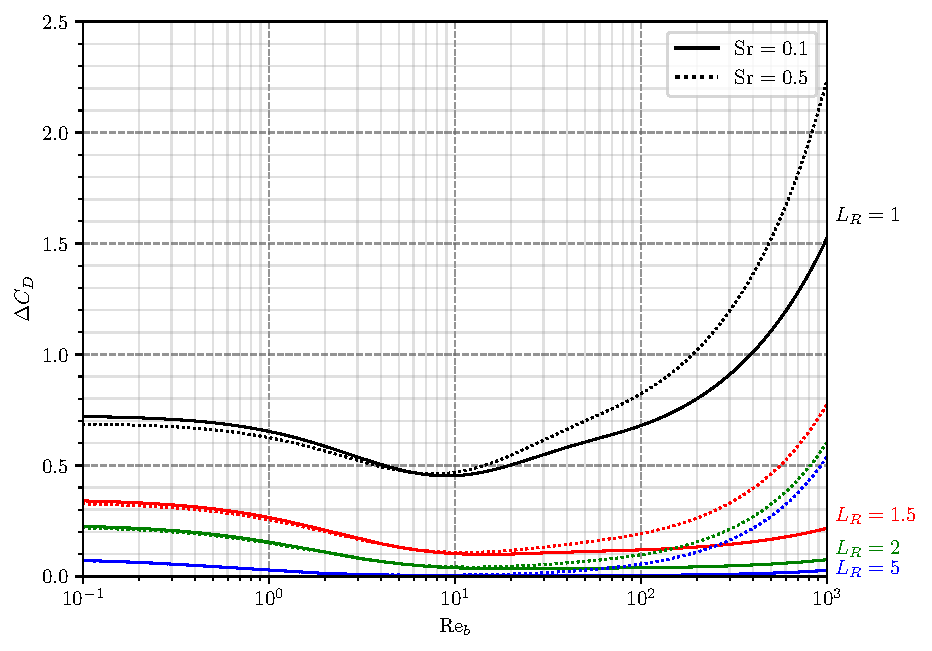
\includegraphics[width=0.8\linewidth]{img/forces/corr_drag.pdf}
\caption{Drag correction from Shi \etal [Shi].}
\label{fig:CD_shi}
\end{figure}





\begin{table}[H]
\scriptsize
\centering
\begin{center}
{\setlength{\tabcolsep}{7pt}
{\renewcommand{\arraystretch}{1.5}
\begin{tabular}{|p{2mm}|p{6mm}|p{17mm}|p{17mm}|p{17mm}|p{17mm}|p{17mm}|p{17mm}|}
\hline 
 & & \multicolumn{6}{|c|}{Authors} \\
\hline
 & & Klausner & Thorncroft & Sugrue & Mazzocco & Ren & Present \\
\hline
\multirow{6}*{\rotatebox{90}{Forces}} &  $\vect{F_{B}}$ & Eq. \ref{eq:buoyancy} & Eq. \ref{eq:buoyancy} & Eq. \ref{eq:buoyancy} & Eq. \ref{eq:buoyancy} & Eq. \ref{eq:buoyancy} & Eq. \ref{eq:buoyancy} \\
   %\cline{2-4}
& $\vect{F_{C}}$ & [Klausner] & [Klausner] & [Klausner] & [Klausner] & [Klausner] & [Klausner]  \\
  %\cline{2-4}  
& $\vect{F_{CP}}$ & Eq. \ref{eq:FCP} &  Eq. \ref{eq:FCP} &  Eq. \ref{eq:FCP} &  Eq. \ref{eq:FCP} & Eq. \ref{eq:FCP} & Eq. \ref{eq:FCP}  \\
 %\cline{2-4}
& $\vect{F_{D}}$ & [Mei] & [Mei] & [Mei] & [Zeng] $\times $ 0.66 & [Mei] & [Shi] + [Mei]  \\
& $\vect{F_{L}}$ & a & a & a & a & a & [Shi]  \\
& \multirow{3}*{$\vect{F_{AM}}$} & {RPE,\newline $\theta_{i}=\pi/17$} & {RPE,\newline $\theta_{i}=\pi/17$} & {RPE,\newline $\theta_{i}=\pi/17$} & {RPE, $\cos{\theta_{i}}=1$, $\sin{\theta_{i}}=0.2$ }& {RPE,\newline $\theta_{i}=\pi/17$} & {Potential flow [VdG] \newline + Lagrange equation} \\
\hline
\end{tabular}}}
\label{BdF_summ}
\caption{Summary of different force-balance mechanistic approaches}
\label{tab:all_BdF}
\end{center}
\end{table}




\begin{figure}[h!]
\centering
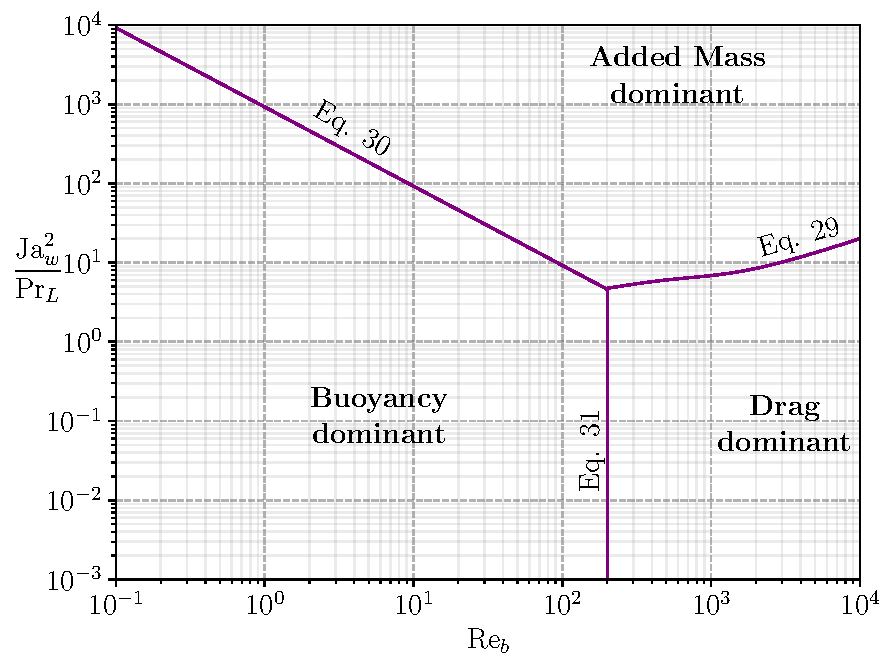
\includegraphics[width=1.0\linewidth]{img/forces/ND_map1.pdf}
\caption{Dominance map regarding departure by sliding. Boundaries plotted for water at 1 bar and $D_{d}=0.5$mm.}
\label{fig:ND_map1}
\end{figure}





\begin{figure}[h!]
\centering
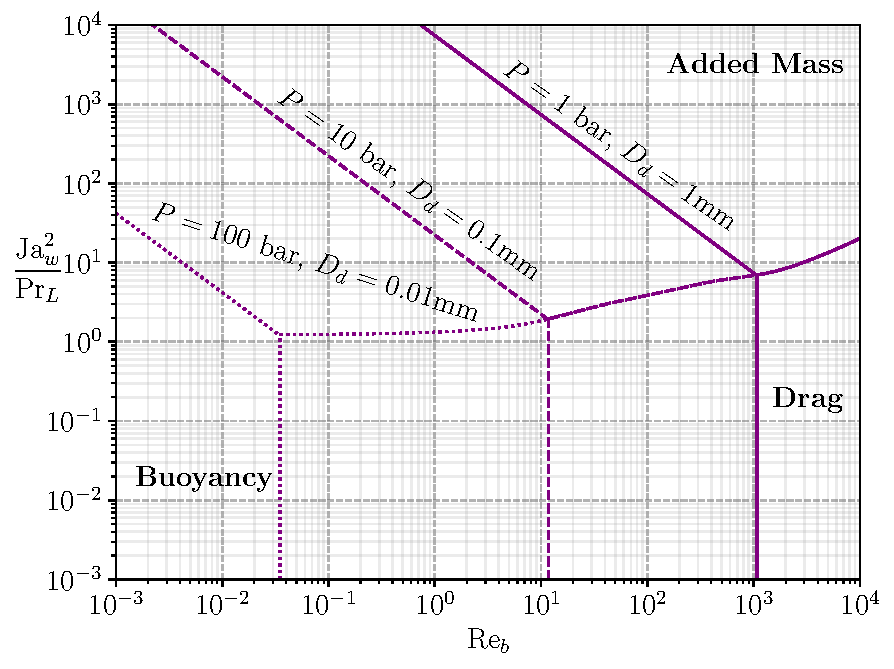
\includegraphics[width=1.0\textwidth]{img/forces/press_map.pdf}
\caption{Dominance map plotted for water at different pressures and bubble departure diameters.}
\label{fig:press_map}
\end{figure}





\begin{figure}[h!]
\centering
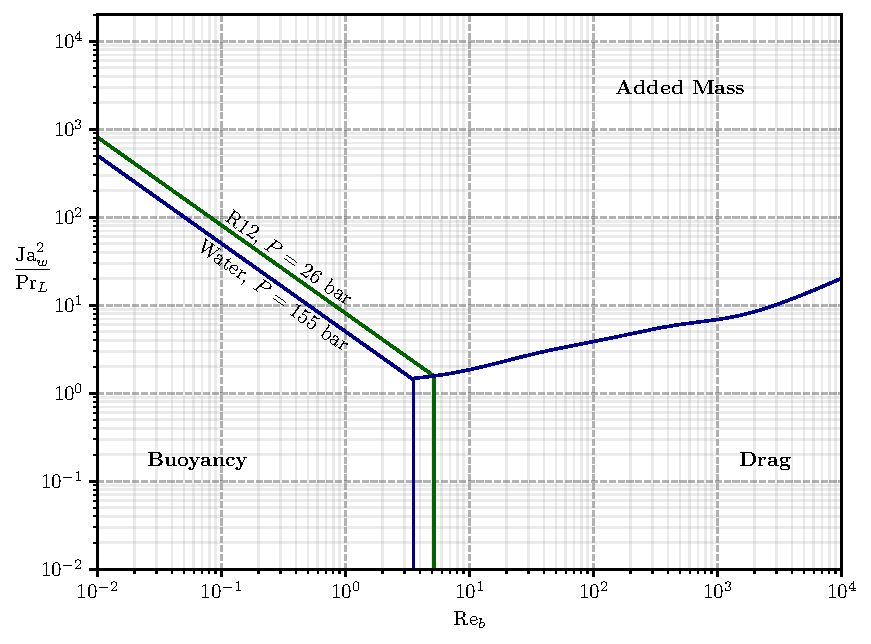
\includegraphics[width=1.0\linewidth]{img/forces/R12_PWR.pdf}
\caption{Dominance map for R12 as simulating fluid for PWR. $D_{d}=0.05$mm is chosen according to R12 measurements from Garnier \etal[Garnier] who found bubbles of $\sim 0.1$mm diameter after lift-off.}
\label{fig:R12_PWR}
\end{figure}






\begin{table}[h!]
\scriptsize
\centering
\begin{tabular}{|c||c|c|c|c||c|c|} \hline
Author &  $D_{h}$ [mm] & $G_{L}$ [$\debm$] & $\Delta T_{w}$ [K] & $D_{d}$ [mm]  & $\Re_{b}$ (-) & $\Ja_{w}^{2}/\Pr$ (-)\\
\hline
\hline
Sugrue \etal[Sugrue] & 16.642 & 250 - 400 & 2 - 6 & 0.229 - 0.391 & 139.1 - 180.1 & 20.57 - 185.2 \\
\hline
Guan \etal[Guan] & 9 & 87.3 - 319.2 & 4.5 - 8.5 & 0.62 - 1.85 & 193.3 - 923.4& 104.2 - 371.6 \\
\hline
Maity[Maity] & 20 & 0 - 239.6 & 5 - 5.9 & 0.788 - 1.713 & 186.6 - 516.7 & 128.6 - 179.06 \\
\hline
\end{tabular}
\caption{Thermal-hydraulics parameters range for the low pressure data.}
\label{tab:lowP_data}
\end{table}




\begin{figure}[h!]
\begin{center}
\subfloat[Sugrue data]{
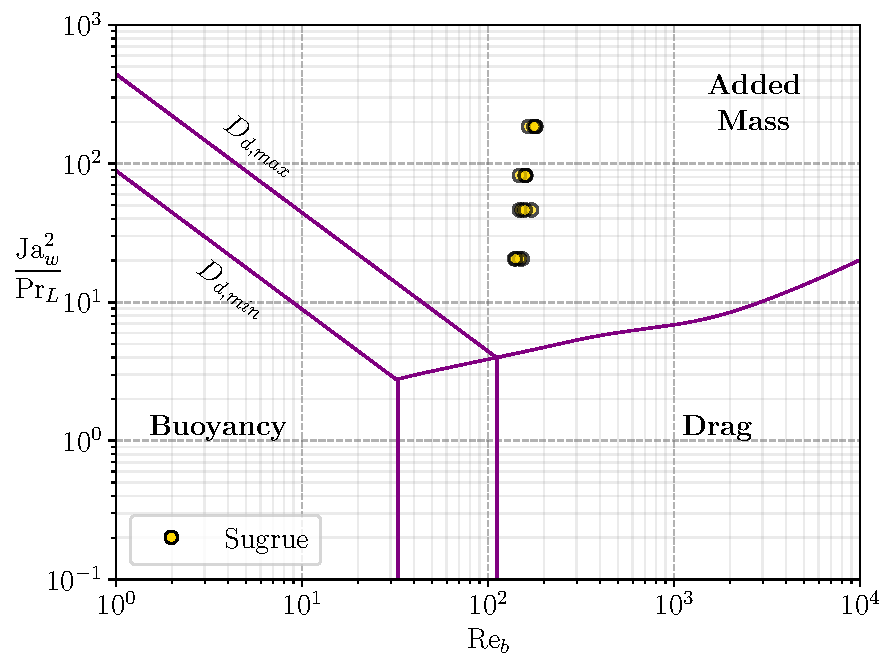
\includegraphics[width=0.5\linewidth]{img/forces/sugrue.pdf}
} 
\subfloat[Guan data]{
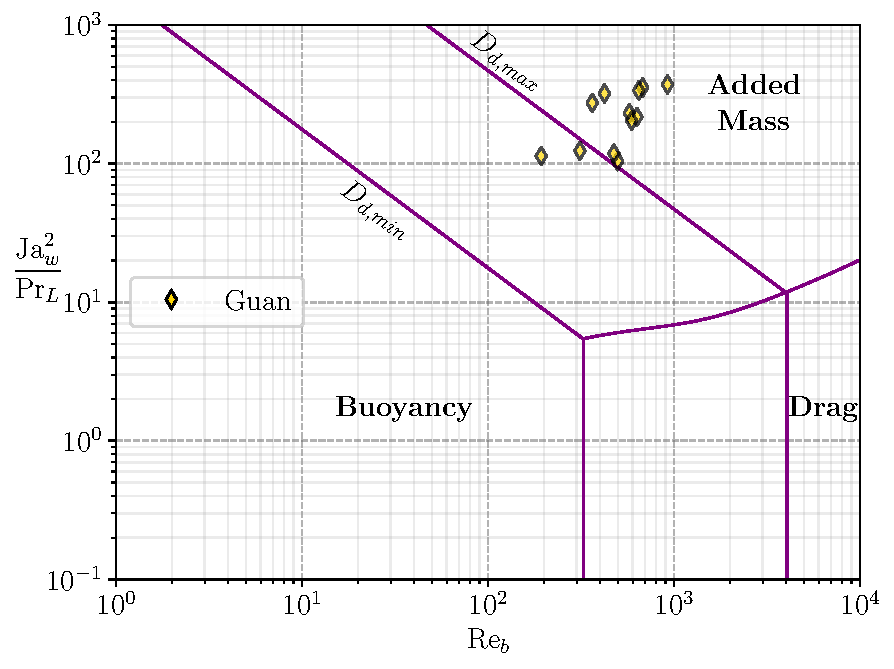
\includegraphics[width=0.5\linewidth]{img/forces/guan.pdf}
}
\\
\subfloat[Maity data]{
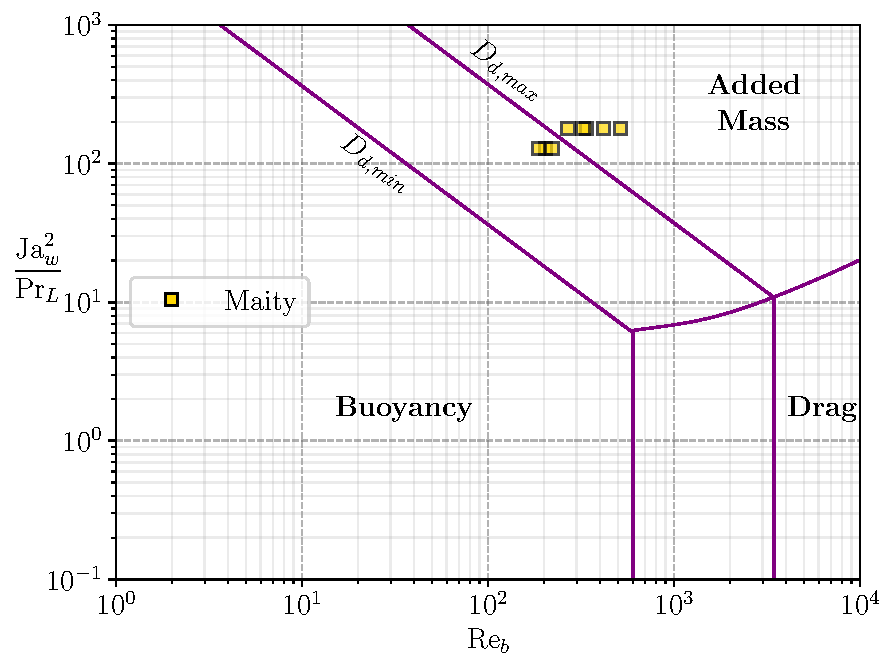
\includegraphics[width=0.5\linewidth]{img/forces/maity.pdf}
}

	\caption{Dominance maps for each low pressure data sets.}	
	\label{fig:lowP_maps}
\end{center}
\end{figure}






\begin{table}[h!]
\scriptsize
\centering
\begin{tabular}{|c||c|c|c|c|c||c|} \hline
Author &  $D_{h}$ [mm] & $G_{L}$ [$\debm$] & $P$ [Bar]  & $\phi_{w}$ [MW.m\up{-2}] & $D_{d}$ [mm]  & $\Re_{b}$ [-] \\
\hline
\hline
\multirow{2}*{Kossolapov[Kossolapov]} & \multirow{2}*{11.78} &  \multirow{2}*{500-1500} & 19.9 & 0.178 - 0.495 & 0.021 - 0.047 & 43.9 - 110.2\\
 &  &  &  39.8  & 0.291 - 0.613 & 0.01 - 0.035 & 17.0 - 55.9\\
\hline
\end{tabular}
\caption{Thermal-hydraulics parameters range for Kossolapov data.}
\label{tab:highP_data}
\end{table}





\begin{figure*}[h!]
\centering
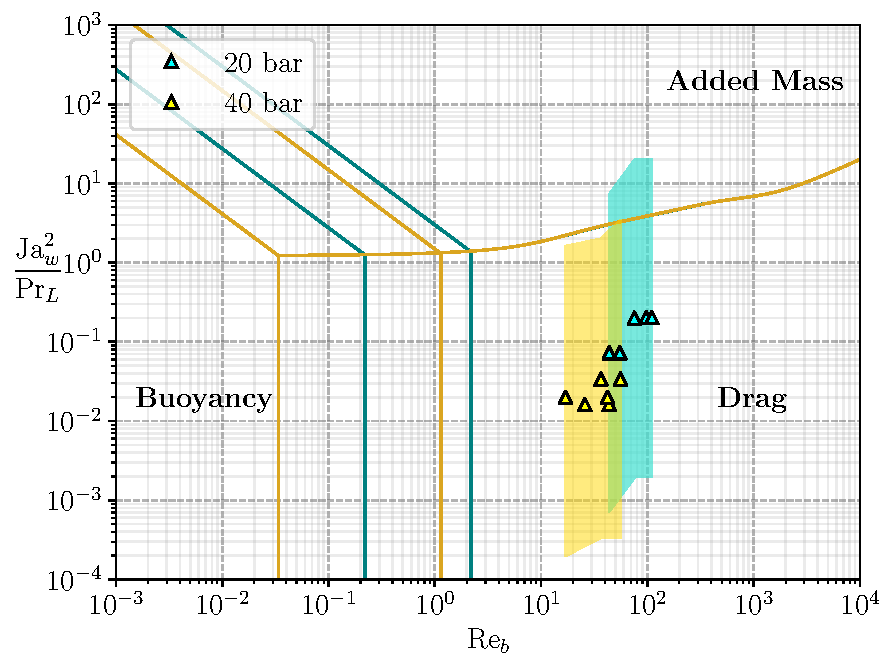
\includegraphics[width=0.7\textwidth]{img/forces/kossmap_all.pdf}
\caption{Dominance map for high pressure measurements from Kossolapov}
\label{fig:highP_map}
\end{figure*}




\begin{figure*}[h!]
\centering
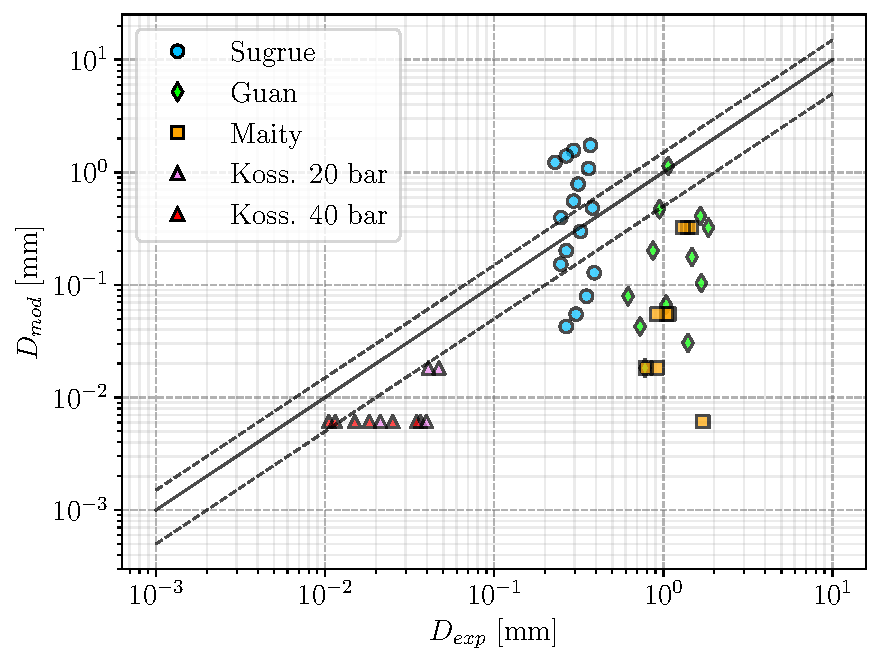
\includegraphics[width=0.7\textwidth]{img/forces/pred_nogr.pdf}
\caption{$D_{d}$ predictions using Eq. \ref{eq:pred_nogr}}
\label{fig:pred_nogr}
\end{figure*}




\begin{figure*}[h!]
\centering
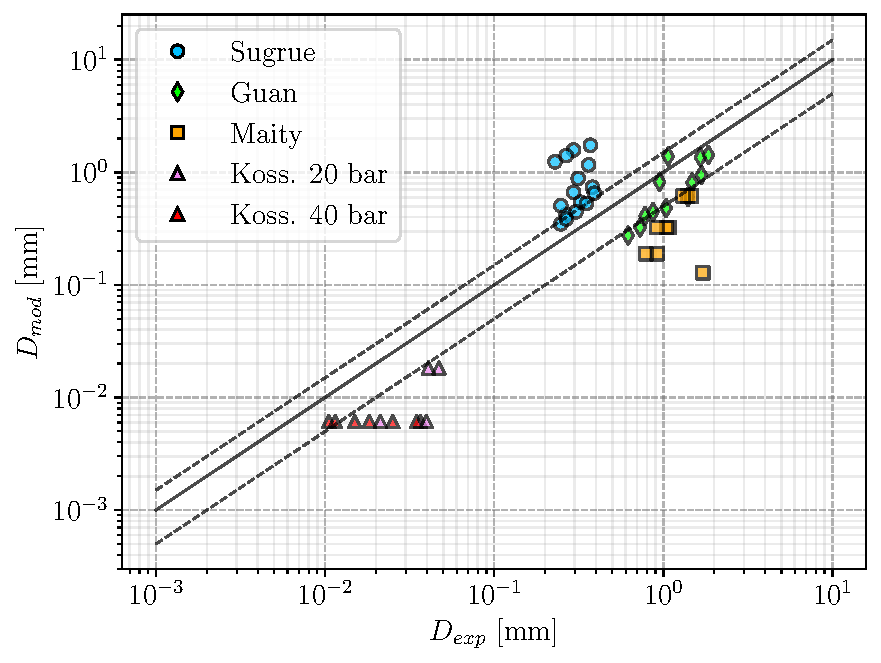
\includegraphics[width=0.7\textwidth]{img/forces/pred_gr.pdf}
\caption{$D_{d}$ predictions using Eq. \ref{eq:pred_gr}}
\label{fig:pred_gr}
\end{figure*}



\begin{figure}[h!]
\begin{center}
\subfloat[Using Eq.\ref{eq:pred_nogr}]{
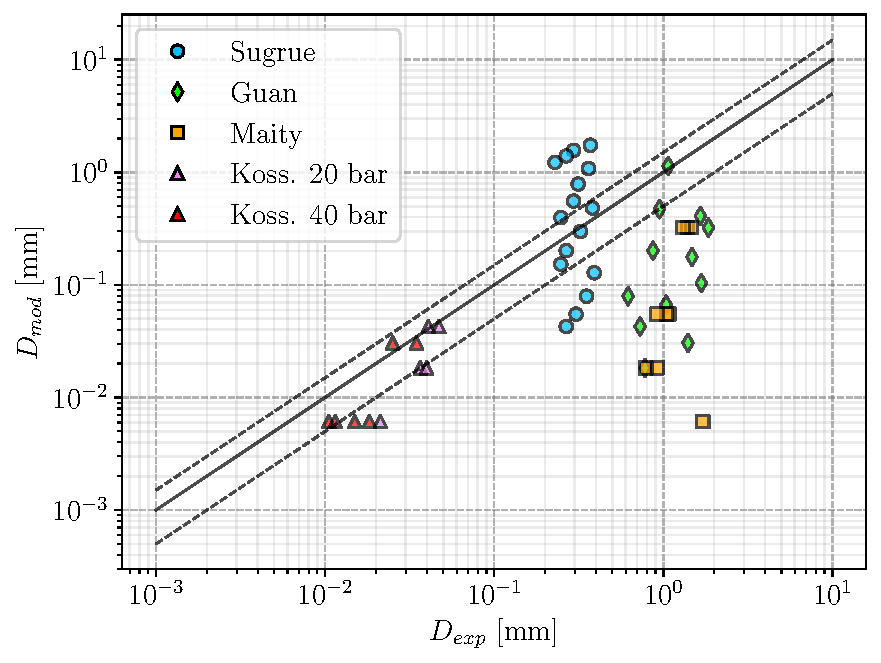
\includegraphics[width=0.5\linewidth]{img/forces/pred_nogrKoss4deg.pdf}
} 
\subfloat[Using Eq.\ref{eq:pred_gr}]{
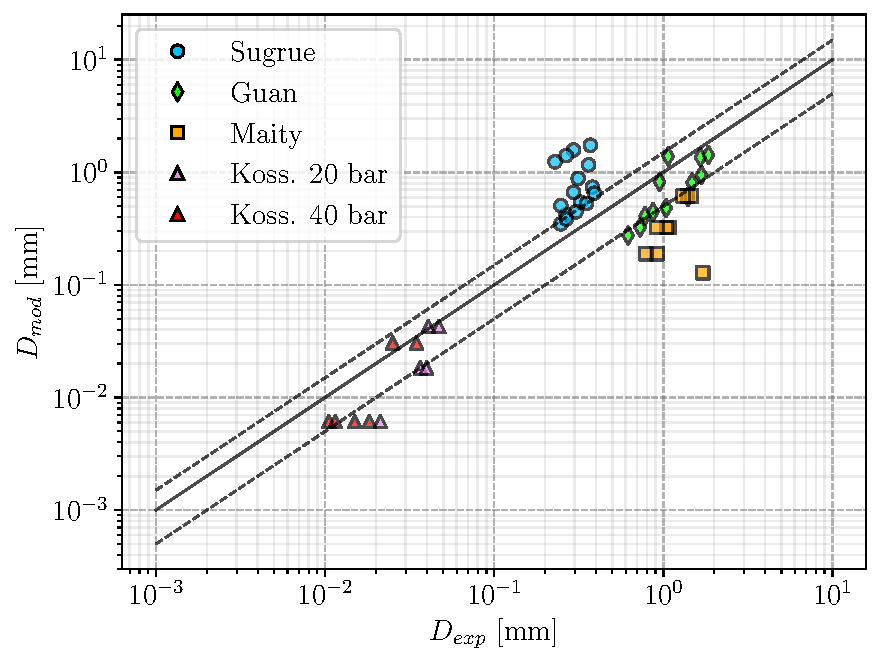
\includegraphics[width=0.5\linewidth]{img/forces/pred_grKoss4deg.pdf}
}
	\caption{$D_{d}$ predictions using $\dtheta = 4\degree$ for Kossolapov}	
	\label{fig:pred_Koss4deg}
\end{center}
\end{figure}




\begin{figure}[h!]
\begin{center}
\subfloat[$\Delta T_{w}=5.0$\degree C, $G_{L}=73.8~\debm$]{
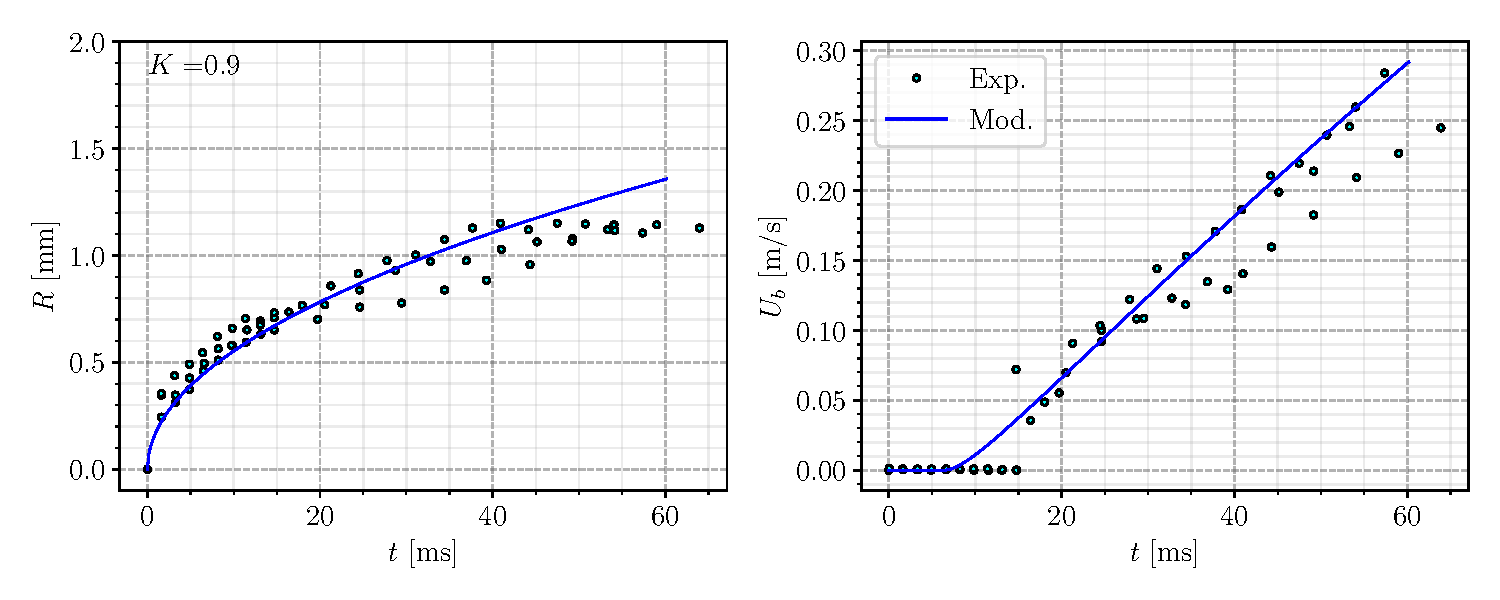
\includegraphics[width=0.9\linewidth]{img/forces/maity_V0p077.pdf}
} 
\\
\subfloat[$\Delta T_{w}=5.9$\degree C, $G_{L}=143.8~\debm$]{
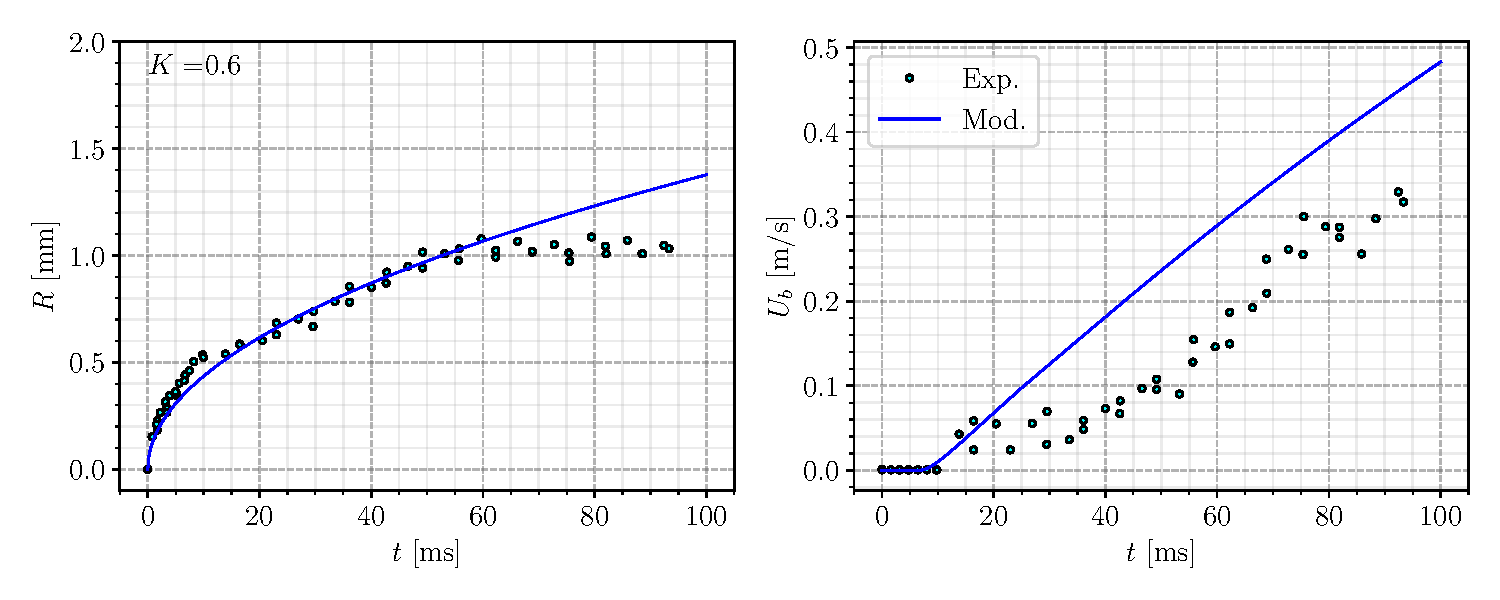
\includegraphics[width=0.9\linewidth]{img/forces/maity_V0p15.pdf}
}
\\
\subfloat[$\Delta T_{w}=5.9$\degree C, $G_{L}=239.6~\debm$]{
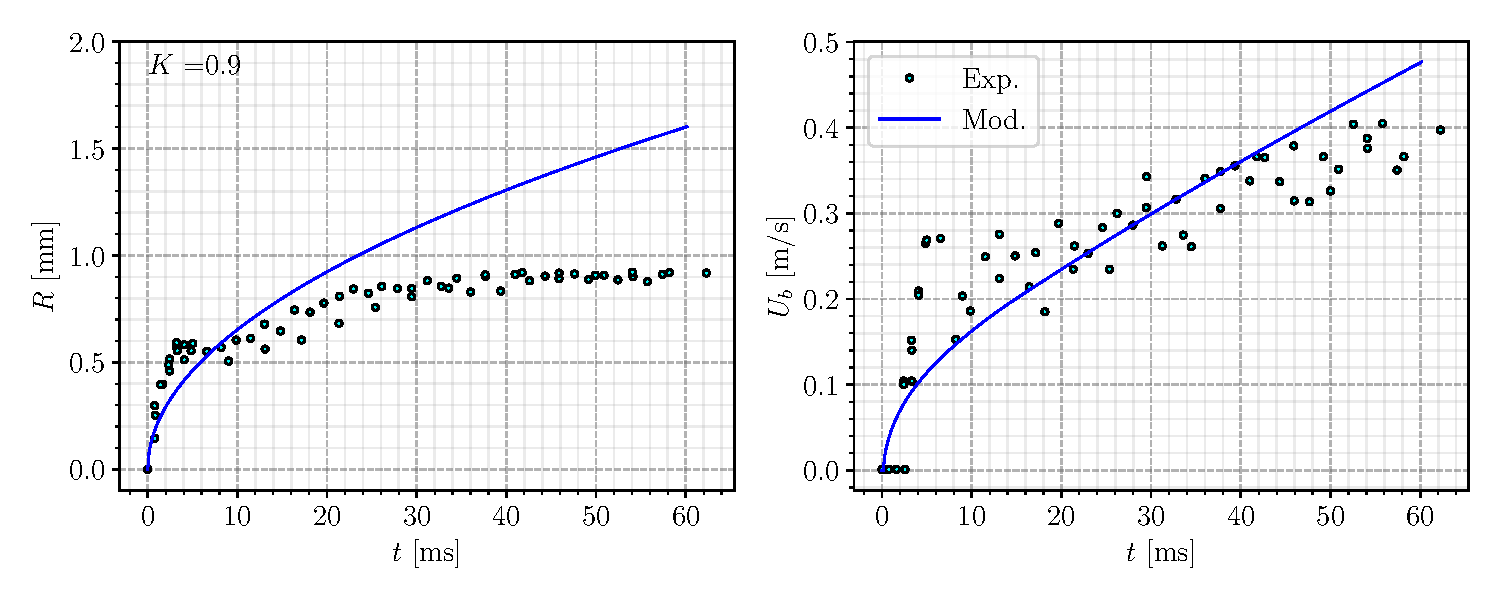
\includegraphics[width=0.9\linewidth]{img/forces/maity_V0p25.pdf}
}
	\caption{Bubble sliding velocity predictions on Maity cases}
	\label{fig:slide_maity}
\end{center}
\end{figure}



\begin{figure}[h!]
\begin{center}
\subfloat[$\phi_{w}=0.178$~MW/m\up{2}, $G_{L}=500~\debm$]{
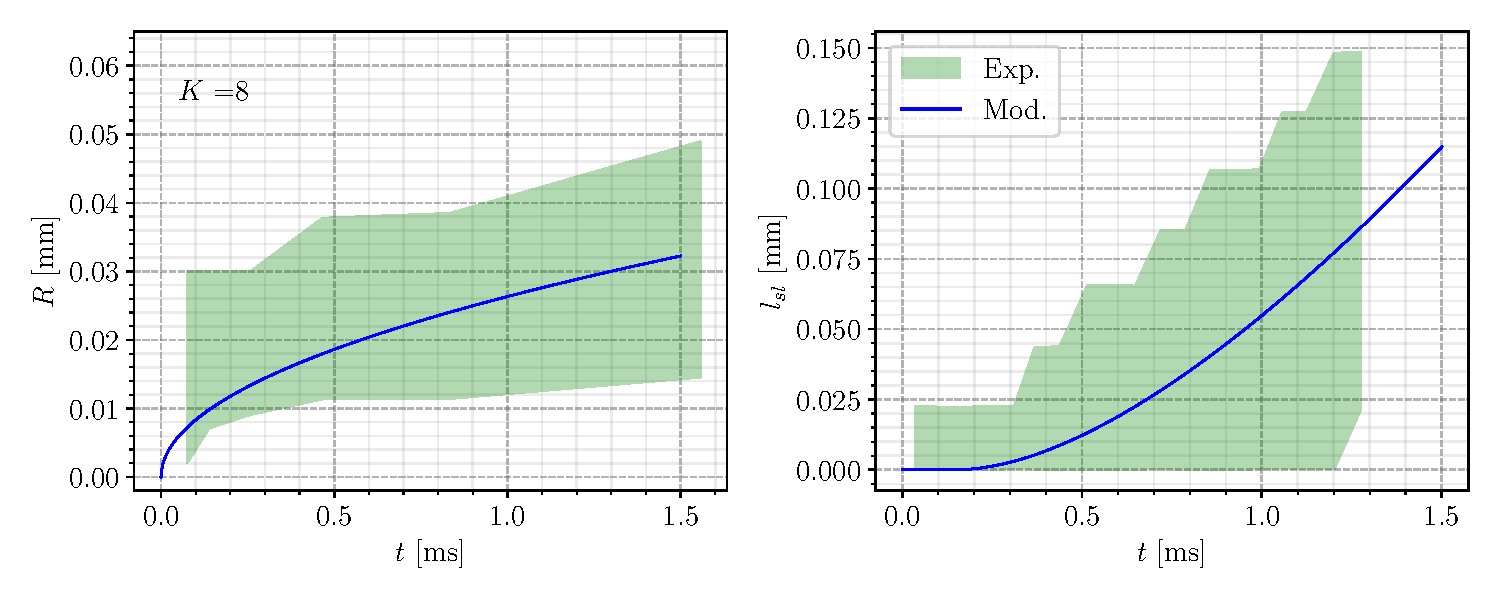
\includegraphics[width=0.9\linewidth]{img/forces/Koss_P20_G500.pdf}
} 
\\
\subfloat[$\phi_{w}=0.495$~MW/m\up{2}, $G_{L}=994~\debm$]{
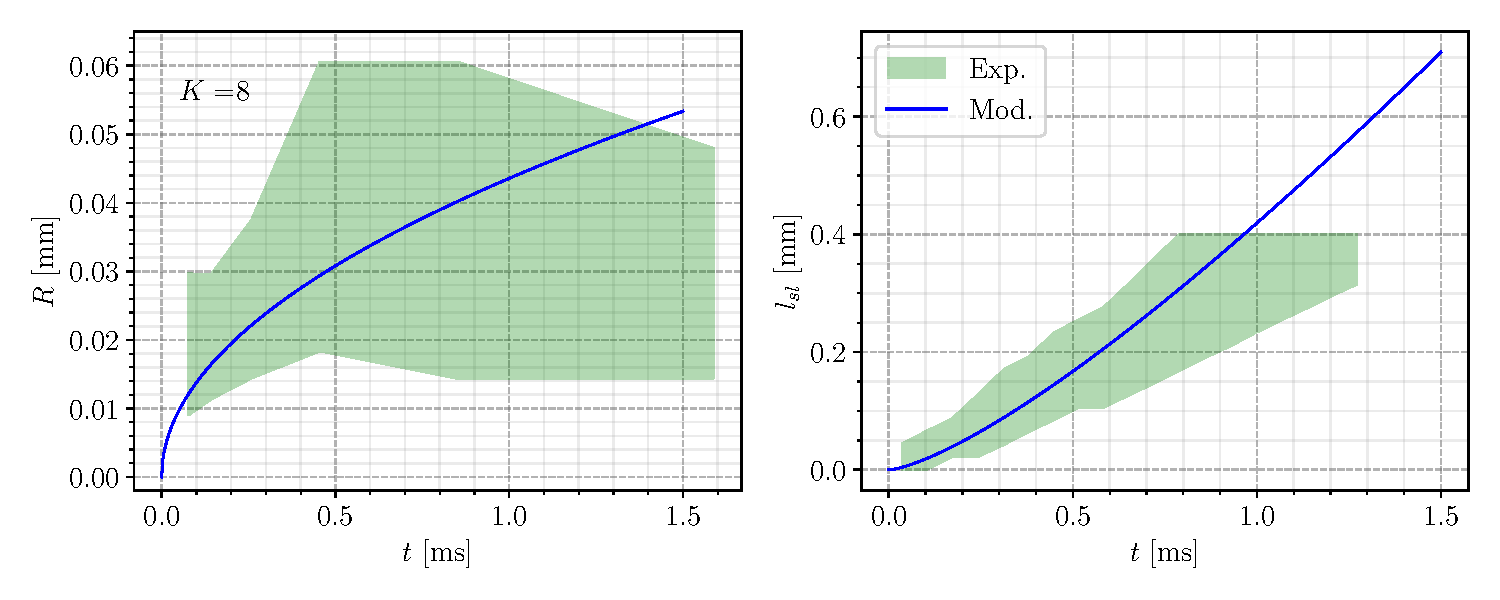
\includegraphics[width=0.9\linewidth]{img/forces/Koss_P20_G1000.pdf}
} 
\\
\subfloat[$\phi_{w}=0.487$~MW/m\up{2}, $G_{L}=1504~\debm$]{
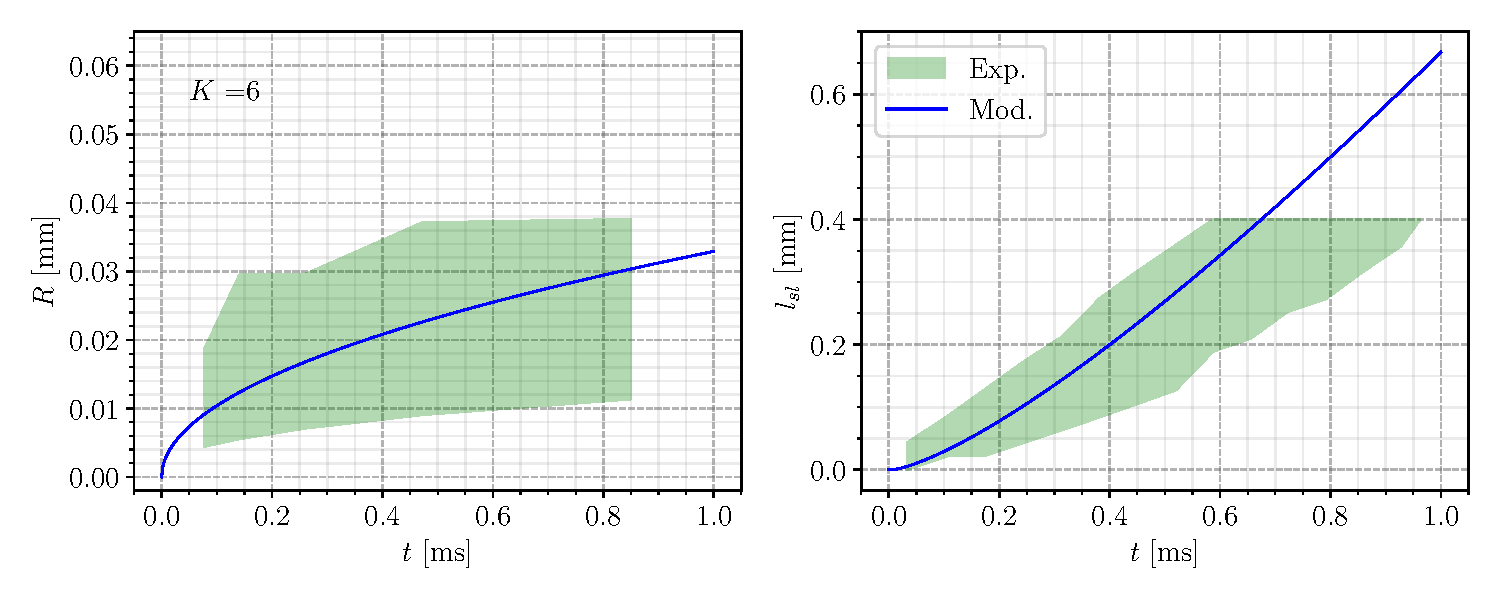
\includegraphics[width=0.9\linewidth]{img/forces/Koss_P20_G1500.pdf}
} 
	\caption{Bubble sliding length predictions on Kossolapov cases - $P=20$ bar}
	\label{fig:slide_koss_20bar}	
\end{center}
\end{figure}


\begin{figure}[h!]
\begin{center}
\subfloat[$\phi_{w}=0.291$~MW/m\up{2}, $G_{L}=500~\debm$]{
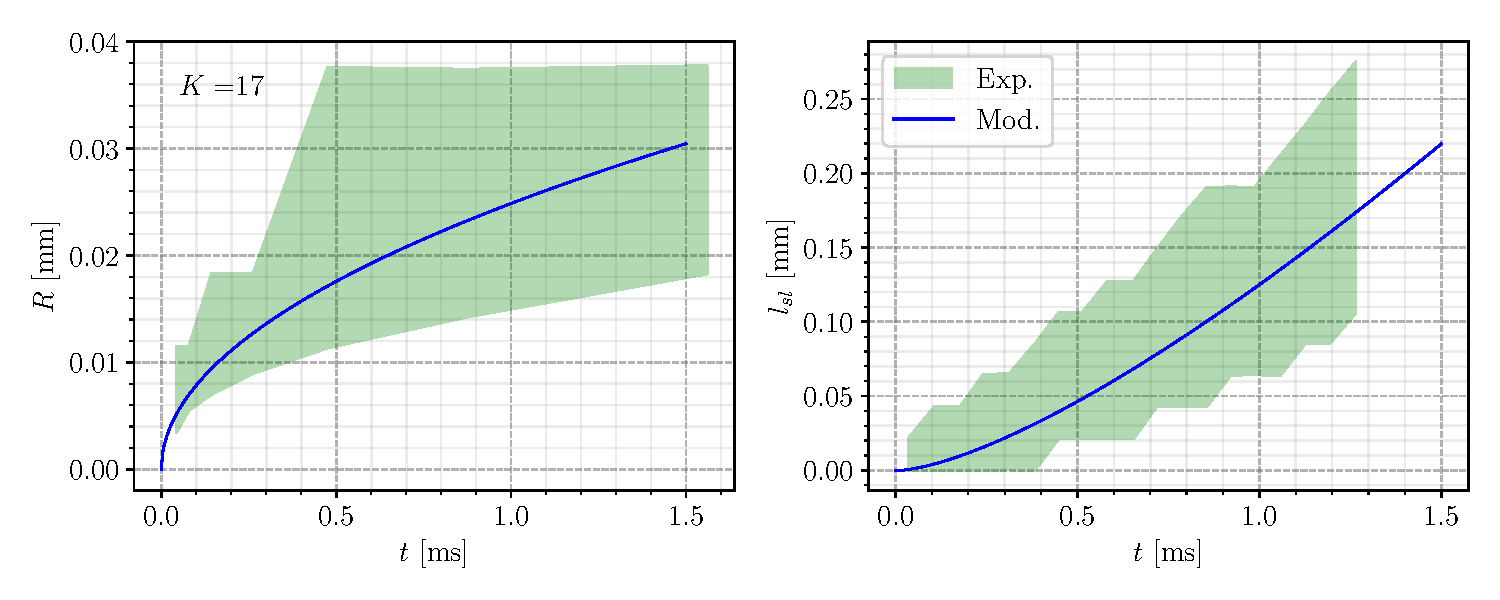
\includegraphics[width=0.9\linewidth]{img/forces/Koss_P40_G500.pdf}
} 
\\
\subfloat[$\phi_{w}=0.361$~MW/m\up{2}, $G_{L}=994~\debm$]{
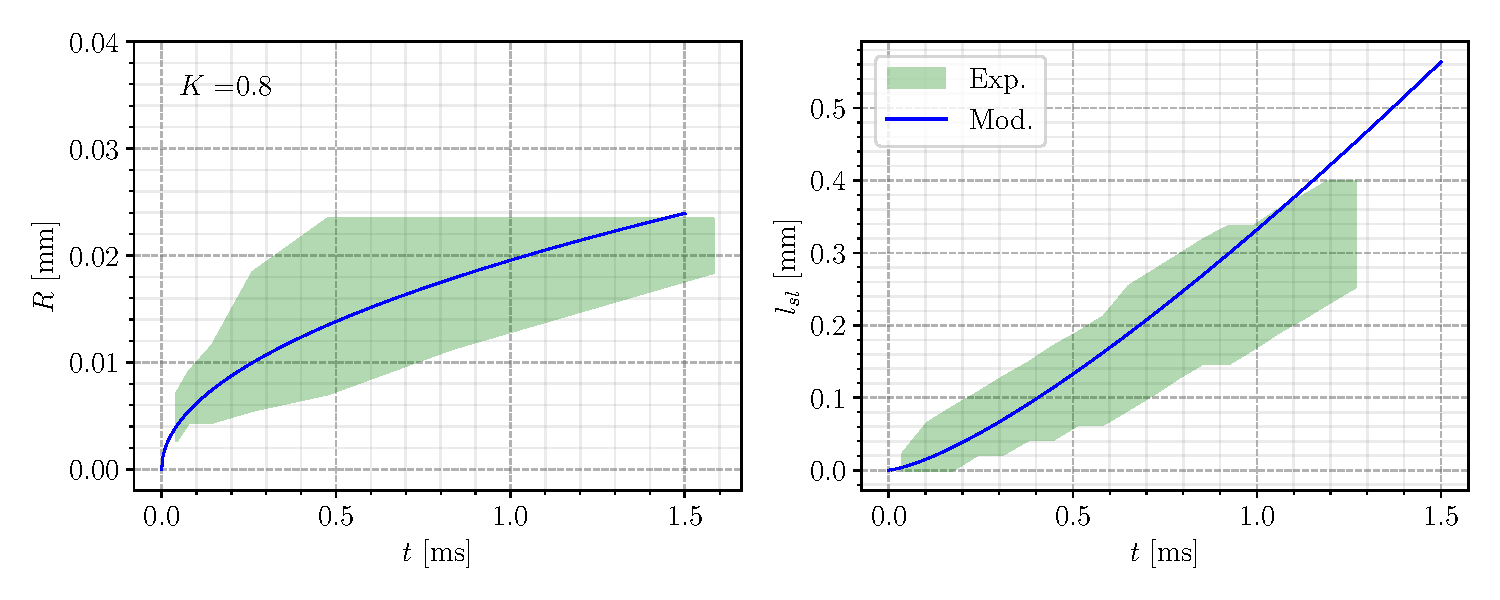
\includegraphics[width=0.9\linewidth]{img/forces/Koss_P40_G1000.pdf}
} 
\\
\subfloat[$\phi_{w}=0.613$~MW/m\up{2}, $G_{L}=1504~\debm$]{
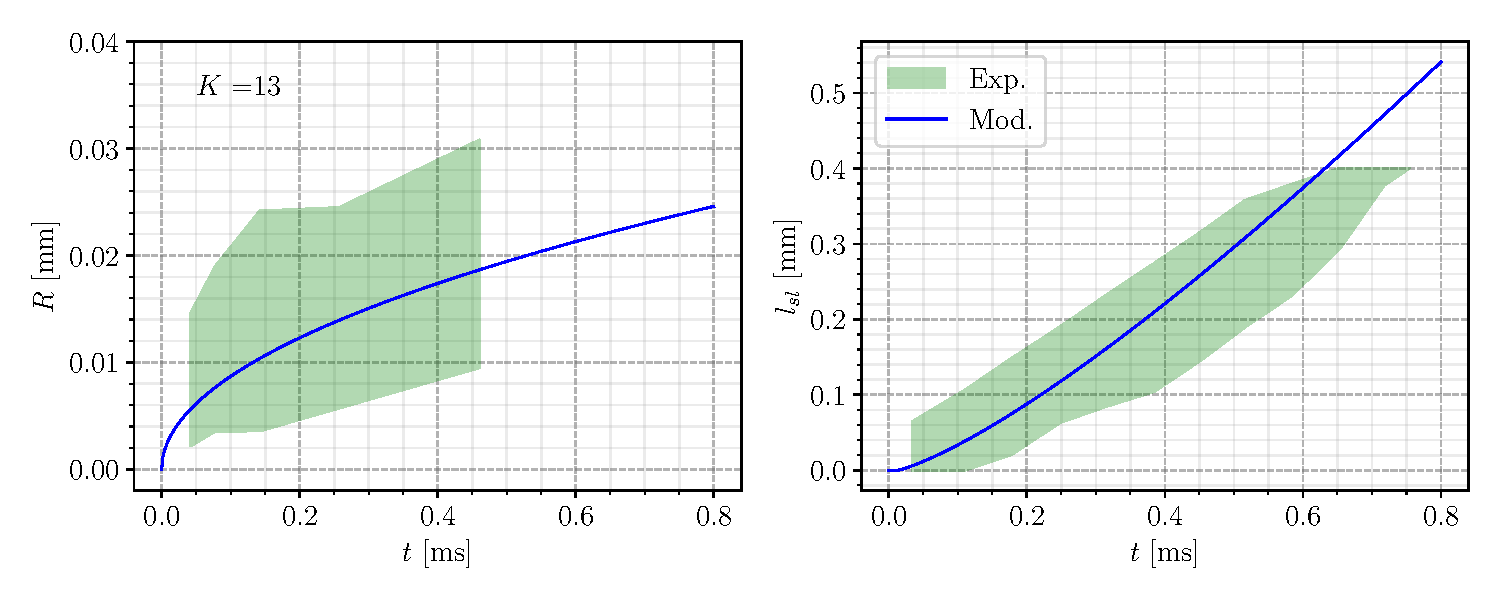
\includegraphics[width=0.9\linewidth]{img/forces/Koss_P40_G1500.pdf}
} 
	\caption{Bubble sliding length predictions on Kossolapov cases - $P=40$ bar}	
	\label{fig:slide_koss_40bar}
\end{center}
\end{figure}






\clearpage





\newpage

\newpage

When trying to understand the underlying physics behind departure and lift-off of growing bubbles on a wall, forces naturally come into the equations. Indeed, the critical diameters at which a bubble will leave its nucleation site to slide or lift-off from the surface are directly linked to the force balance applied to this very bubble.

\npar

Many authors have previsouly been tackling this issue to try to derive the whole force balance experienced by a bubble, starting with Klausner in 1993[CITE]. Since then, mechanistic approaches have been thoroughly studied to overcome empirical, correlation-based estimations of bubble departure and lift-off diameters[CITE]. The underlying idea is that if one manages to precisely compute the force balance applied to a bubble, it would lead to a high-fidelity representation of the bubble dynamics to evaluate its departure diameter $D_{d}$, sliding length $l_{sl}$, sliding velocity $U_{b}$ and lift-off diameter $D_{lo}$.  

\npar

However, the variety of hydrodynamics phenomena experienced by a boiling bubble in a flow makes the derivation of its force balance a very complicated task, in not impossible. This can only be achieved under many assumptions regardig bubble shape, external flow, etc. Moreover, the triggering of departure and lift-off can be associated to critical values of the force balance since many authors consider that the bubble starts moving when the balance is broken in one direction[CITE]. It is actually very delicate since it implies detecting a very small change in the whole force balance ($\sim \mathrm{nN}$) resulting from the sum of forces of much greater magnitude ($\sim \mu\mathrm{N}$)[CITE].

\npar

Nevertheless, studying the force balance can still provide interesting insights on bubble dynamics, particularly when comparing the impact of different forces depending on the operating conditions. That is why this chapter is dedicated to an analysis of the boiling bubble dynamics to try to understand a bit further the bubble behavior regarding the departure and sliding phenomenon in vertical flow boiling.



\begin{figure}[h!]
\centering

\fbox{


\begin{tikzpicture}[scale=3.0, every node/.style={scale=0.7}]


%%%Truncated sphere on a vertical wall

\coordinate (O1) at (0,0);
\coordinate (O2) at (0,2);

\draw (O1)--(O2);

\coordinate (Ob) at (0,1.0);

\tikzmath{\thet = 45; \thetrad= \thet * pi / 180; \ray=0.5; \rw=\ray * sin(\thetrad r);};


\coordinate (Oarc) at ($(Ob)-(0,{\ray * sin(\thetrad r)})$);
\draw (Oarc) arc({(-pi+\thetrad ) r}:{(pi-\thetrad ) r}:\ray);

%Upstream angle
\draw (Oarc) --++(-90+\thet:0.3);
\draw ($(Oarc)+(0,-0.15)$) arc(-90:-90+\thet:0.15) node[near end, below]{$\theta$};

%%Downstream angle
%\coordinate (Oarc2) at ($(Oarc) - (2*\rw,0)$);
%\draw (Oarc2) --++(180-\thet:0.3);
%\draw ($(Oarc2)+(-0.15,0)$) arc(180:180-\thet:0.15) node[near end, left]{$\alpha$};

%Center and radius

\coordinate (Cb) at ($(Ob)+({\ray*cos(\thetrad r)},0 )$);
\draw (Cb) node{$\times$} node[below right]{$O$};

\draw[densely dashed, <->, >=latex] (Cb) -- (Oarc) node[midway, below right]{$R$};


%%Forces

\draw[->, >=latex, violet!70!black] (Ob)--++(\ray/2,0) node[near end, above]{$\vect{F_{CP}}$};

\draw[->, >=latex, red!70!black!] ($(Cb)+(\ray,0)$)--++(\ray/2,0) node[very near end, above]{$\vect{F_{L}}$};
\draw[->, >=latex, red!70!black!] ($(Cb)+(0,\ray)$)--++(0,\ray/2) node[very near end, right]{$\vect{F_{D}}$};

\coordinate (Oarc2) at ($(Oarc)+(0,{2*\rw})$);
\draw[->, >=latex, violet] (Oarc)--++(90+\thet:\ray/2) node[very near end, above]{$\vect{F_{C}}$};
\draw[->, >=latex, violet] (Oarc2)--++(-90-\thet:\ray/2) node[very near end, below]{$\vect{F_{C}}$};

\draw[->, >=latex, blue!70!black] (Cb)--++(0,\ray/1.5) node[very near end, right]{$\vect{F_{B}}$};


\draw[->, >=latex, green!50!black!] (Cb)--++(90+\thet/1.5:\ray/1.5) node[very near end, above]{$\vect{F_{AM}}$};

%Gravity

\draw[->, >=latex, blue!30!black]  ($(Cb)+({1.5*\ray},{1.5*\ray})$)--++(0,-\ray/2) node[very near end, right]{$\vect{g}$};


%Flow arrows
\foreach \i in {2,...,14} 
{
\coordinate (Oloc) at ($(O1)+(\i/15,0.05)$);
\draw[->,>=latex, gray!70!blue] (Oloc)--++(0,{ln(1+0.03*\i)});
}
\draw[gray!70!blue] ($(Oloc)+(0.1,0.1)$) node{$\vect{U_{L}}$};

%Referential vectors
\coordinate (Ovect) at (1.75,0);
\draw[->, >=latex] (Ovect)--++(0.3,0) node[very near end, above right]{$\vect{e_{y}}$};
\draw[->, >=latex] (Ovect)--++(0,0.3) node[very near end, above right]{$\vect{e_{x}}$};




%Tilted bubble
\coordinate (Ob2) at (2.5,1.0);

\coordinate (O1) at (2.5,0);
\coordinate (O2) at (2.5,2);
\draw (O1)--(O2);

\tikzmath{\thet = 40; \thetrad= \thet * pi / 180;
\dthet=10; \dthetrad=\dthet*pi/180;
\thetadvrad=\thetrad - \dthetrad;
\thetrecrad=\thetrad + \dthetrad;
\thetadv=\thetadvrad*180/pi;
\thetrec=\thetrecrad*180/pi;
\ray=0.5; 
\rayadv=\ray *(1+cos(\thetrad r))/(1+ cos(\thetadvrad r);
\rayrec=\ray *(1+cos(\thetrad r))/(1+ cos(\thetrecrad r);};

\coordinate (Oarc) at ($(Ob2)-(0,{\ray * sin(\thetrad r)})$);


\draw (Oarc) arc({-pi+(\thetrecrad)) r}:{0 r}:\rayrec) arc ({0 r}:{pi-(\thetadvrad)) r}:\rayadv);

%Upstream angle
\draw (Oarc) --++(-90+\thetrecrad r:0.3) node[very near end, below]{$\theta + \dtheta$};
\draw ($(Oarc)+(0,-0.15)$) arc(-90:-90+\thetrecrad r:0.15) ;

%Downstream angle
\coordinate (Oarc2) at ($(Oarc) + (0,{\rayadv * sin(\thetadvrad r) + \rayrec * sin(\thetrecrad r)})$);
\draw (Oarc2) --++({90-(\thetadvrad r)}:0.3);
\coordinate (angadv) at ($(Oarc2) +({90-(\thetadvrad r)}:0.3)$);
\draw (angadv)  node[above]{$\theta - \dtheta $};
\draw ($(Oarc2)+(0,+0.15)$) arc(90:{90-(\thetadvrad r)}:0.15);



%Center and radius

\coordinate (Cb) at ($(Oarc2)+( {\ray * cos(\thetrad r)} , {-0.5 * (\rayadv * sin(\thetadvrad r) + \rayrec  * sin(\thetrecrad r) )})$);
\draw (Cb) node{$\times$} node[below right]{$O$};

\draw[densely dashed, <->, >=latex] (Cb) -- (Oarc) node[midway, above left]{$R$};


%Inclination angle

%\draw[densely dotted] (Cb) --++ (0.7,0);
%\draw[densely dotted] (Cb) --++ ({(1*\dthetrad r)}: 0.7 );
%\draw ($(Cb) + (0.3,0)$) arc(0: {(\dthetrad r)}:0.3)  node[midway, right]{$\dtheta$};
%
%



%%Forces

\draw[->, >=latex, violet!70!black] (Ob2)--++(\ray/2,0) node[near end, above]{$\vect{F_{CP}}$};

\draw[->, >=latex, red!70!black!] ($(Cb)+(\ray,0)$)--++(\ray/2,0) node[very near end, above]{$\vect{F_{L}}$};
\draw[->, >=latex, red!70!black!] ($(Cb)+(0,-\rayadv*0.95)$)--++(0,-\ray/2) node[very near end, right]{$\vect{F_{D}}$};
\draw[->, >=latex, red] ($(Cb)+(0,+\rayrec*1.04)$)--++(0,+\ray/2) node[very near end, right]{$\vect{U_{b}}$};


\draw[->, >=latex, violet] (Oarc)--++(90+\thetrec:\ray/2) node[very near end, above]{$\vect{F_{C}}$};
\draw[->, >=latex, violet] (Oarc2)--++(-90-\thetadv:\ray/2) node[very near end, below]{$\vect{F_{C}}$};

\draw[->, >=latex, blue!70!black] (Cb)--++(0,\ray/1.5) node[very near end, right]{$\vect{F_{B}}$};


\draw[->, >=latex, green!50!black!] (Cb)--++(90-\thet:-\ray/1.5) node[very near end, right]{$\vect{F_{AM}}$};

%Gravity

\draw[->, >=latex, blue!30!black]  ($(Cb)+({1.5*\ray},{1.5*\ray})$)--++(0,-\ray/2) node[very near end, right]{$\vect{g}$};



%Flow arrows
\foreach \i in {2,...,14} 
{
\coordinate (Oloc) at ($(O1)+(\i/15,0.05)$);
\draw[->,>=latex, gray!70!blue] (Oloc)--++(0,{ln(1+0.03*\i)});
}
\draw[gray!70!blue] ($(Oloc)+(0.1,0.1)$) node{$\vect{U_{L}}$};



\end{tikzpicture}

}

\caption{Bubble force balance in vertical flow boiling}
\end{figure}


\section{Establishment of the force balance for a bubble on a vertical wall }


In this section, we wish to detail expressions of the different forces experienced by the bubble and to compare their magnitude in order to assess which will be predominant in the departure and lift-off process.

\subsection{Bubble shape : Geometrical definitions}

\label{subsec:geom_bub}

In order to clearly express each of the considered forces, assumptions regarding the shape of the bubble nucleating at the wall are needed.

\npar

Here, we assume that the bubbles will mostly have the shape of a truncated sphere with respect to the contact angle $\theta_{s}$ (Fig. \ref{fig:bub_shape}), being a thermophysical property of the fluid and the  wall. This assumption can thoroughly be discussed since many experimental measurements and visualizations have shown that in the case of low pressure boiling, bubbles tend te be strongly deformed depending on the flow conditions (\textsc{Maity}, \textsc{Estrada-Pérez} \etal, etc.) thus casting doubts on spherical or quasi-spherical hypotheses.

\npar
On the other hand, experiments conducted by \textsc{Kossolapov} found that in vertical flow boiling, increasing pressure leads to smaller and less deformable bubbles. Thus, supposing a truncated spherical shape could be relevant to model nucleating bubbles on a heater surface. Moreover, working on highly deformed bubbles would undoubtedly imply complicated calculations and extra parameters to account for.

\textsc{Kossolapov}'s measurements also concluded that bubbles' inclination due to the flow nearly disappears at high pressures. However, since bubble tilt plays a great role in the surface tension force, we consider an angle tilt $\dtheta$ compared to the static contact angle $\theta_{s}$.

\begin{figure}[h!]
\centering
\fbox{

\renewcommand{\dalpha}{\text{d}\alpha}

\begin{tikzpicture}[scale=4.0, every node/.style={scale=0.7}]


\coordinate (O) at (0,0);
\coordinate (A2) at (1.4,0);
\coordinate (A) at (3.2,0);


%Sections and wall
\draw (O) -- (A);
%\draw ($(O)-(0,0.05)$) -- ($(A)-(0,0.05)$);
%\foreach \i in {0,...,15}
%{
%\draw (\i*0.2,0) -- (\i*0.2+0.1,-0.05);
%}

\draw[dashed, gray!70!white] (A2) --++ (0,1);


%Non-tilded bubble
\coordinate (Ob) at (0.75,0);

\tikzmath{\alph = 40; \alphrad= \alph * pi / 180; \ray=0.5; \rw=\ray * sin(\alphrad r); \h=\ray * cos(\alphrad r);};


\coordinate (Oarc) at ($(Ob)+({\ray * sin(\alphrad r)},0)$);
\draw (Oarc) arc({-(pi/2-\alphrad) r}:{(pi+pi/2-\alphrad) r}:\ray);

%Right angle
\draw (Oarc) --++(\alph:0.3);
\draw ($(Oarc)+(0.15,0)$) arc(0:\alph:0.15) node[near end, right]{$\theta_{s}$};

%Left angle
\coordinate (Oarc2) at ($(Oarc) - (2*\rw,0)$);
\draw (Oarc2) --++(180-\alph:0.3);
\draw ($(Oarc2)+(-0.15,0)$) arc(180:180-\alph:0.15) node[near end, left]{$\theta_{s}$};

%Center and radius

\coordinate (Cb) at ($(Ob)+(0,{\ray*cos(\alphrad r)} )$);
\draw (Cb) node{$\times$} node[above right]{$O$};

\draw[densely dashed, <->, >=latex] (Cb) -- (Oarc2) node[midway, above left]{$R$};


%Angular portion

\draw[densely dotted] (Cb)--++(0,\ray);
\draw[densely dotted] (Cb) -- (Oarc);

\draw ($(Cb)+(0,0.3)$) arc(90:-(90-\alph):0.3) node[midway, right]{$\Theta$};

%Bubble foot
\draw[<->,>=latex, densely dashed] ($(Oarc)-(0,0.02)$) --++ (-\rw,0) node[midway,below]{$r_{w}$};
%Bubble height
\draw[<->, >=latex, densely dashed] (Cb)--++(0,-\h) node[midway, right]{$h$};


%Tilted bubble
\coordinate (Ob2) at (2.25,0);

\tikzmath{\alph = 40; \alphrad= \alph * pi / 180;
\dalph=20; \dalphrad=\dalph*pi/180;
\alphadvrad=\alphrad - \dalphrad;
\alphrecrad=\alphrad + \dalphrad;
\ray=0.5; 
\rayadv=\ray *(1+cos(\alphrad r))/(1+ cos(\alphadvrad r);
\rayrec=\ray *(1+cos(\alphrad r))/(1+ cos(\alphrecrad r);};

\coordinate (Oarc) at ($(Ob2)+({\ray * sin(\alphrad r)},0)$);


\draw (Oarc) arc({-(pi/2-(\alphadvrad)) r}:{(pi/2) r}:\rayadv) arc ({(pi/2) r}:{(pi+pi/2-(\alphrecrad)) r}:\rayrec);

%Right angle
\draw (Oarc) --++(\alphadvrad r:0.3);
\draw ($(Oarc)+(0.15,0)$) arc(0:\alphadvrad r:0.15) node[midway, right]{$\theta_{s} - \dtheta$};

%Left angle
\coordinate (Oarc2) at ($(Oarc) - ({\rayadv * sin(\alphadvrad r) + \rayrec * sin(\alphrecrad r)},0)$);
\draw (Oarc2) --++({180-(\alphrecrad r)}:0.3);
\draw ($(Oarc2)+(-0.15,0)$) arc(180:{180-(\alphrecrad r)}:0.15) node[midway, left]{$\theta_{s} + \dtheta $};



%Center and radius

\coordinate (Cb) at ($(Oarc)+( -{0.5 * (\rayadv * sin(\alphadvrad r) + \rayrec  * sin(\alphrecrad r) } , {\ray * cos(\alphrad r)} )$);
\draw (Cb) node{$\times$} node[below right]{$O$};

\draw[densely dashed, <->, >=latex] (Cb) -- (Oarc2) node[midway, above left]{$R$};


%Inclination angle

\draw[densely dotted] (Cb) --++ (0,0.7);
\draw[densely dotted] (Cb) --++ ({90 - (1*\dalphrad r)}: 0.7 );
\draw ($(Cb) + (0,0.3)$) arc(90: {90 - (\dalphrad r)}:0.3)  node[midway, above]{$\dtheta$};



%Flow arrows
\foreach \i in {2,...,14} 
{
\coordinate (Oloc) at ($(A2)+(0.05,\i/15)$);
\draw[->,>=latex, gray!70!blue] (Oloc)--++({ln(1+0.03*\i)},0);
}



\end{tikzpicture}

}
\caption{Sketch of the supposed bubble shape with (right) and without inclination (left).}
\label{fig:bub_shape}

\end{figure}



The resulting bubble's volume $V_{b}$ and projected area in the direction of the flow $S_{p}$ can then be computed using the spherical coordinates system and defining the total angular portion covered by the bubble as $\Theta = \pi - \theta_{s}$, the bubble foot radius $r_{w}=R \sin{\theta_{s}}$ and the distance between the center of the bubble and the surface $h=R\parth{1+\cos{\theta_{s}}}$, we have :

\begin{align}
V_{b} &= \underbrace{ \int_{r=0}^{R} \int_{\theta=0}^{\Theta} \int_{\varphi=0}^{2\pi} r^{2}\sin{\theta} \text{d}r ~\text{d}\theta~ \text{d}\varphi }_{\text{Spherical volume}}+ \underbrace {\frac{1}{3}\pi r_{w}^{2}h}_{\text{Conic volume}}
=\frac{4}{3}\pi R^{3} \crocht{ \frac{1}{4} \parth{2-\cos{\theta_{s}}}\parth{1+\cos{\theta_{s}}}^{2} } \\
S_{p}&= \underbrace{\int_{r=0}^{R}\int_{\theta=-\Theta}^{\Theta}r \text{d}r ~ \text{d}\theta}_{\text{Circular area}} + \underbrace{r_{w}h}_{\text{Triangular area}} = \pi R^{2} \crocht{1-\frac{\theta_{s}}{\pi} + \frac{\sin{2\theta_{s}}}{2\pi} } 
\end{align}


Thus, we can define shape factors that represent the ratio between the volume and projected areas of the truncated sphere compared to a complete sphere : 

\begin{align}
f_{V}\left(\theta_{s}\right)=\frac{V_{ts}}{V_{s}}=\frac{1}{4}\left(2-\cos{\theta_{s}}\right)\left(1+\cos{\theta_{s}}\right)^{2}\\
f_{S_{p}}\left(\theta_{s}\right)=\frac{S_{p,ts}}{S_{p,s}}=1-\frac{\theta_{s}}{\pi}+\frac{\sin{2\theta_{s}}}{2\pi}
\end{align}

Subscripts $s$ and $ts$ respectively denoting spherical and truncated spherical shapes.


\npar

Using those assomptions, we can thus express the volume of vapor generated for a single bubble up to its lift-off diameter $D_{lo}=2R_{lo}$ (Eq. \ref{eq:boil_vol}) :

\begin{align}
\label{eq:boil_vol}
V_{b}=\frac{4}{3}\pi \bluemath{R_{lo}}^{3} f_{V}\parth{\theta_{s}} = \frac{\pi \bluemath{D_{lo}}^{3}}{6} f_{V}\parth{\theta_{s}}
\end{align}

As described in Section \ref{subsec:geom_bub}, we consider a bubble with a potential inclination $\dalpha$ from the static contact angle $\theta_{s}$. Thus, the downstream contact angle is $\theta_{d}=\theta_{s} - \dtheta$ and the upstream contact angle is $\theta_{u}=\theta_{s} + \dtheta$ (Figure \ref{fig:bub_shape}).

\npar

To estimate the bubble foot radius $r_{w}$ of such a bubble, we can express it as the average between the two foot diameters for the advancing and receding contact angles :

\begin{align}
r_{w} &= \frac{1}{2}\parth{\sin{\theta_{d}}R + \sin{\theta_{u}}R} = R~\sin{\theta_{s}}\cos{\dtheta}
\end{align}

\npar

In the following subsections, the vectors $\vect{e_{\|}}$ and $\vect{e_{\bot}}$ respectively represent the colinear and orthogonal vector to the wall surface.


\begin{figure}[h!]


\begin{tikzpicture}[yscale=3, xscale=2]

\tikzmath{\alph1=70;}
\draw[gray!90!] (0,0) grid[ystep=1,xstep=pi/2](pi,1);
\draw[gray!60!, dashed] (0,0) grid[ystep=0.5, xstep=pi/8](pi,1);
%\draw[gray!60!, densely dotted] (0,0) grid[step=pi/4](4,1);


%\draw [domain=-pi:pi] plot (\x,{sin(\x r)});
%\draw[domain=0:pi] plot(\x, {cos(\x r)});
\draw [domain=0:pi, red] plot(\x,{0.25*(2-cos(\x r))*((1+cos(\x r))^2)}); %f_V
\draw [domain=0:pi, olive!80!black] plot(\x,{1-\x/pi + sin((2*\x) r)/(2*pi)}); %f_Sp
%\draw [domain=0:pi, blue] plot(\x,{(1-cos(\x r)^2)}); %f_G

\draw[->,>=latex,black] (0,0)--(0,1.1) node[very near end, above=0.3cm]{$\redmath{f_{V}}$, $\greenmath{f_{S_{p}}}$} node[very near start, below=0.4cm]{$0$} node[very near end, left]{$1$};
\draw[->,>=latex,black] (0,0)--(pi+0.1,0) node[very near end, below=0.2cm, right=0.8cm]{$\theta_{s}$};

\draw (pi/4,0) node[below]{$\pi/4$};
\draw (pi/2,0) node[below]{$\pi/2$};
\draw (3*pi/4,0) node[below]{$3\pi/4$};


\end{tikzpicture}
\hfill
\begin{tikzpicture}[xscale=2, yscale=1.5]

\tikzmath{\alphdeg=45; \alphrad=\alphdeg*pi/180;}
\draw[gray!90!] (0,-1) grid[xstep=pi/2,ystep=1](pi,1);
\draw[gray!60!, dashed] (0,-1) grid[xstep=pi/8,ystep=0.5](pi,1);

%\draw [domain=-pi:pi] plot (\x,{sin(\x r)});
%\draw[domain=0:pi] plot(\x, {cos(\x r)});
\draw [domain=0:pi, red] plot(\x,{(sin(\alphrad r)^2)*(cos(\x r)^2)}); %f_cp
\draw [domain=0.001:pi, olive!80!black] plot(\x,{(sin(\alphrad r)^2)*sin(2*\x r)/(2*\x)}); %f_s,orth
\draw [domain=0:pi, blue] plot(\x,{1.215*\x*(sin(\alphrad r)^2)*(cos(\x r)^2)/((pi/2)^2 - \x^2)}); %f_s,parl


\draw[->,>=latex,black] (0,-1)--(0,1.1) node[very near end, above=0.5cm]{$\redmath{f_{cp}}$, $\greenmath{f_{s,\bot}}$, $\bluemath{f_{s,\|}}$};
\draw (0,0) node[left]{$0$};
\draw (0,1) node[left]{$1$};
\draw (0,-1) node[left]{$-1$};
\draw[->,>=latex,black] (0,-1)--(pi+0.1,-1) node[very near end, below=0.2cm, right=0.8cm]{$\dtheta$};

\draw (pi/4,-1) node[below]{$\pi/4$};
\draw (pi/2,-1) node[below]{$\pi/2$};
\draw (3*pi/4,-1) node[below]{$3\pi/4$};

\draw[orange!70!black] (\alphrad, -1) -- (\alphrad,1) node[very near end, above=0.5cm]{$\theta_{s}$};

\end{tikzpicture}
\caption{Representation of the shape functions}
\end{figure}


\subsection{Buoyancy force}

The well-known buoyancy force, also called Archimedes force, is computed by integration of the hydrostatic pressure exterted by the liquid over the bubble's surface and results in the difference between the gravity forces experienced by the vapour bubble and the equivalent liquid volume. The expression of this force $\vect{F_{B}}$ is aligned with the gravity vector $\vect{g}=-g\vect{e_{x}}$.

\begin{align}
\vect{F_{B}}&=V_{b}\parth{\rho_{V}-\rho_{L}}\vect{g}=\frac{4}{3}\pi R^{3}f_{V}\parth{\theta_{s}}\parth{\rho_{L}-\rho_{V}}g\vect{e_{x}}
\end{align}

\subsection{Contact Pressure force}

The contact pressure force arises due to the pressure difference between the center of the bubble and the surrounding liquid. This pressure jump can be computed using \textsc{Laplace}'s expression $\Delta P = 2\sigma / R_{c}$ where $R_{c}$ is the curvature radius of the bubble's interface, being equal to $R$ in the case of a spherical bubble. This pressure difference is then applied over the bubble foot area and results in a repelling force from the bubble's point of view, giving the resulting expression of $\vect{F_{CP}}$.

\begin{align}
\vect{F_{CP}}&=\frac{2\sigma}{R_{c}}\frac{\pi d_{w}^{2}}{4}\vect{e_{y}} \approx 2\sigma \pi R \underbrace{\sinsq{\theta} \cossq{\dtheta}}_{f_{CP}}\vect{e_{\bot}} =2\pi R \sigma f_{CP}\parth{\theta, \dtheta}\vect{e_{x}}\\
\end{align}

\subsection{Capillary force}

The capillary or surface tension force results from the integration of the effort exerted over the triple contact line between the vapor inside the bubble, the surrounding liquid and the wall. This force has been derived by \textsc{Klausner}[CITE] for a inclined bubble, yielding for each direction regarding the wall :

\begin{align}
\vect{F_{C}}&=-1.25 d_{w}\sigma \frac{\pi\parth{\theta_{u}-\theta_{d}}}{\pi^{2}-\parth{\theta_{u}-\theta_{d}}^{2}}\parth{\sin{\theta_{u}}+\sin{\theta_{d}} }\vect{e_{x}} -d_{w} \sigma \frac{\pi}{\theta_{u}-\theta_{d}}\parth{\cos{\alpha_{d}}- \cos{\alpha_{u}}}\vect{e_{y}} \\
%
&\approx -\pi R \sigma \underbrace{\crocht{1.25\ \frac{2\dtheta}{\parth{\frac{\pi}{2}}^{2}-\dtheta^{2}}\sin{\theta_{s}}^{2}\cos{\dtheta}^{2}}}_{f_{C,x}} \vect{e_{x}} - \pi R \sigma \underbrace{\crocht{2\ \sin{\theta_{s}}^{2}\frac{\sin{2\dtheta}}{2\dtheta}}}_{f_{C,y}}\vect{e_{y}}\\
%
&= -\pi R \sigma f_{C,x}\parth{\theta_{s}, \dtheta}\vect{e_{x}} - \pi R \sigma f_{C,y}\parth{\theta_{s}, \dtheta} \vect{e_{y}}
\end{align}

\npar

\subsection{Added Mass force of a growing bubble}

Added mass effects are experienced by the bubble :

\begin{itemize}
\item when its boundary is moving during its growth
\item when accelerating while sliding on the wall 
\item when the surrounding liquid is accelerating
\end{itemize}

We consider a spherical cap shaped bubble standing on a plane wall and facing an uniform liquid velocity $U$. In this situation, Van Der Geld derived the potential flow around the bubble and expressed the liquid kinetic energy, obtaining : 

\begin{align}
T_{L}=\rho_{L}V_{b}\parth{ \frac{1}{2}\alpha \dot{y}^{2} + \frac{1}{2} \trb\dot{R}^{2}+\frac{1}{2}\psi \dot{R}\dot{y} + \frac{1}{2} \alpha_{2} U^{2} }
\end{align}
where $\alpha$, $\mathrm{tr}\parth{\beta}$, $\psi$ and $\alpha_{2}$ are polynomimals of $\lambda = \frac{R}{2h}$. We also have $x$ and $y=h$ denoting the coordinates of the geometrical center of the bubble.

Therefore, we can write those coefficients in the following form : 

\begin{align}
\alpha = \sum_{k=0}^{n}\alpha_{k}\frac{R^{k}}{2^{k}y^{k}}
\end{align}

If we suppose that the generalized coordinates and velocities $x$, $\dot{x}$, $y$, $\dot{y}$, $R$, and $\dot{R}$, we can use the expression of the kinetic energy of the fluid to apply Lagrange's equations to derive the added mass forces on the bubble in both direction parallel and normal to the wall :

\begin{align}
F_{AM,x}&=-\dpartial{}{t}\parth{\dpartial{T_{L}}{\dot{x}}}+\dpartial{T_{L}}{x}\\
F_{AM,y}&=-\dpartial{}{t}\parth{\dpartial{T_{L}}{\dot{y}}}+\dpartial{T_{L}}{y}
\end{align}

In the case of the sliding bubble, we replace the uniform liquid velocity $U$ by the relative velocity experienced by the bubble $U_{rel}=U_{liq}-\dot{x}$ where $U_{liq}$ is the uniform surrounding liquid velocity and $\dot{x}$ the velocity of the center of the bubble, which is the sliding velocity of the bubble. Yielding :



\begin{align}
T_{L}=\frac{\rho_{L}V_{b}}{2}\parth{\alpha \dot{y}^{2} +\mathrm{tr}\parth{\beta}\dot{R}^{2}+\psi \dot{R}\dot{y} +\alpha_{2} \parth{U_{liq}-\dot{x}}^{2} }
\end{align}
 

\paragraph{Added mass in $x$ direction}

Parallel to the wall, since $\lambda$ depends on $y$ and $R$, it is independent of $\dot{x}$, yielding zero-derivatives for the added mass coefficients. We can write :

\begin{align}
\dpartial{T_{L}}{\dot{x}}&=\frac{\rho_{L}V_{b}}{2}\alpha_{2} \dpartial{\parth{ \parth{U_{liq}-\dot{x}}^{2}} }{\dot{x}}\\
&= \rho_{L}V_{b}\alpha_{2}\parth{\dot{x}-U_{liq}}\\
\end{align}\\

As for the time derivatives, we have : 

\begin{align}
\dpartial{V_{b}}{t}&=\dpartial{\frac{4}{3}\pi R^{3}}{t} = 4\pi R^{2} \dot{R}\\
\dpartial{\lambda}{t}&=\frac{\dot{R}~2y-R~2\dot{y}}{4y^{2}}=\lambda\parth{ \frac{\dot{R}}{R} - \frac{\dot{y}}{y}  }=\lambda \parth{\frac{\dot{R}}{R}-2\lambda \frac{\dot{y}}{R}}=\frac{\lambda}{R}\parth{\dot{R}-2\lambda \dot{y}}\\
\dpartial{\alpha}{t}&=\sum_{k=0}^{n}\alpha_{k}\dpartial{\lambda ^{k}}{t} = \sum_{k=0}^{n}\alpha_{k}~k\lambda ^{k-1} \dpartial{\lambda}{t} = \parth{ \frac{\dot{R}}{R} - \frac{\dot{y}}{y}  }\underbrace{ \sum_{k=0}^{n}\alpha_{k}~k\lambda^{k} }_{\tilde{\alpha}} = \frac{1}{R}\parth{\dot{R}-2\lambda \dot{y}}\tilde{\alpha}
\end{align}

Yielding : 

\begin{align}
\dpartial{}{t}\parth{ \dpartial{T_{L}}{\dot{x}}}&=\rho_{L}\crocht{ 4\pi R^{2} \dot{R} \alpha_{2}\parth{\dot{x}-U_{liq}}+\frac{4}{3}\pi R^{3}\parth{ \frac{\dot{R}}{R} - \frac{\dot{y}}{y} }\tilde{\alpha_{2}}\parth{\dot{x}-U_{liq}}+\frac{4}{3}\pi R^{3}\alpha_{2} \ddot{x} } \\
&=4\pi R^{2} \rho_{L}\crocht{ \alpha_{2}\dot{R}\parth{\dot{x}-U_{liq}}+\frac{\tilde{\alpha_{2}}}{3}\parth{\dot{R}- 2\lambda \dot{y} }\parth{\dot{x}-U_{liq}} + \frac{R}{3}\alpha_{2}\ddot{x} }\\
&=4 \pi R^{2} \rho_{L}\crocht{\parth{\alpha_{2}+\frac{\tilde{\alpha_{2}}}{3}}\dot{R}\parth{\dot{x}-U_{liq}}-\frac{2}{3}\lambda \tilde{\alpha_{2}}\dot{y}\parth{\dot{x}-U_{liq}}+\frac{R}{3}\alpha_{2}\ddot{x} }
\end{align}

We also have, with the independence of the variables :

\begin{align}
\dpartial{T_{L}}{x}&=0
\end{align}


Finally yielding, 

\begin{align}
F_{AM,x}=4\pi R^{2}\rho_{L} \crocht{\parth{\alpha_{2}+\frac{\tilde{\alpha_{2}}}{3}}\dot{R}U_{rel}-\frac{2}{3}\lambda \tilde{\alpha_{2}}\dot{y}U_{rel}-\frac{R}{3}\alpha_{2}\ddot{x} }
\end{align}

We can immediately observe that the added mass related to the bubble growth will promote detachment when the bubble is still attached to its nucleation site ($\dot{x}=0$). This contradicts the often-used approach using solely the Rayleigh-Plesset equation projected in both direction using the inclination angle of the bubble. 

The other part of this added-mass force is naturally linked to the acceleration of the bubble and the mass of displaced liquid. 


\paragraph{Added mass in $y$ direction}

Following the same approach normal to the wall, we obtain : 

\begin{align}
\dpartial{T_{L}}{\dot{y}}&=\frac{1}{2}\rho_{L}\frac{4}{3}\pi R^{3}\parth{\alpha 2\dot{y}+\psi\dot{R}}=\rho_{L}\frac{4}{3}\pi R^{3}\parth{\alpha \dot{y} + \frac{\psi}{2}\dot{R}}\\
\nonumber \\
\dpartial{}{t}\parth{\dpartial{T_{L}}{\dot{y}}}&=\rho_{L}4\pi R^{2}\dot{R}\parth{\alpha \dot{y} + \frac{1}{2} \psi \dot{R}}+\rho_{L}\frac{4}{3}\pi R^{3}\parth{\frac{1}{R}\parth{\dot{R}-2\lambda \dot{y}}\tilde{\alpha}\dot{y} +\alpha\ddot{y}+\frac{1}{2}\tilde{\psi}\frac{1}{R}\parth{\dot{R}-2\lambda \dot{y}}\dot{R} +\frac{1}{2}\psi \ddot{R}}\\
&=\rho_{L}4\pi R^{2}\crocht{\frac{\alpha}{3}R\ddot{y}+\frac{\psi}{6}R \ddot{R} + \parth{\frac{\psi}{2} +\frac{\tilde{\psi}}{6}}\dot{R}^{2} -\frac{2}{3}\lambda \tilde{\alpha} \dot{y}^{2} + \parth{ \alpha + \frac{\tilde{\alpha}}{3} - \frac{\tilde{\psi}}{3} }\dot{R}\dot{y} }\\
\nonumber \\
\dpartial{T_{L}}{y}&=\rho_{L}\frac{4}{3}\pi R^{3} \parth{ \frac{1}{2} \dpartial{\alpha}{y}\dot{y}^{2} + \frac{1}{2} \dpartial{\mathrm{tr}\parth{\beta}}{y}\dot{R}^{2}+\frac{1}{2}\dpartial{\psi}{y}\dot{R}\dot{y}+\frac{1}{2}\dpartial{\alpha_{2}}{y}\parth{U_{liq}-\dot{x}}^{2} } 
\end{align}

Where we can write :

\begin{align}
\dpartial{\alpha}{y}=\sum_{k=0}^{n}\alpha_{k}\dpartial{\lambda^{k}}{y} = \sum_{k=0}^{n}\alpha_{k}\frac{R^{k}}{2^{k}}\dpartial{}{y}\parth{\frac{1}{y^{k}}}=\sum_{k=0}^{n}\alpha_{k}\frac{R^{k}}{2^{k}}~\parth{-k}\frac{1}{y^{k+1}}=\frac{1}{y}\sum_{k=0}^{n}\parth{-k}\alpha_{k}\lambda^{k}=-\frac{1}{y}\tilde{\alpha}
\end{align} 

Giving : 

\begin{align}
\dpartial{T_{L}}{y}&=\rho_{L}4\pi R^{2}\frac{R}{6y}\crocht{-\tilde{\alpha}\dot{y}^{2}-\tilde{\mathrm{tr}\parth{\beta}}\dot{R}^{2}-\tilde{\psi}\dot{R}\dot{y}-\tilde{\alpha_{2}}U_{rel}^{2}}\\
&=-\rho_{L}4\pi R^{2}\frac{\lambda}{3}\crocht{\tilde{\alpha}\dot{y}^{2}+\tilde{\mathrm{tr}\parth{\beta}}\dot{R}^{2}+\tilde{\psi}\dot{R}\dot{y}+\tilde{\alpha_{2}}U_{rel}^{2}}
\end{align}

Which finally yields : 

\begin{align}
\nonumber F_{AM,y}=&-\rho_{L}4\pi R^{2}\crocht{\frac{\alpha}{3}R\ddot{y}+\frac{\psi}{6}R \ddot{R} + \parth{\frac{\psi}{2} +\frac{\tilde{\psi}}{6}}\dot{R}^{2} -\frac{2}{3}\lambda \tilde{\alpha} \dot{y}^{2} + \parth{ \alpha + \frac{\tilde{\alpha}}{3} - \frac{\tilde{\psi}}{3} }\dot{R}\dot{y} } \\
&-\rho_{L}4\pi R^{2}\frac{\lambda}{3}\crocht{\tilde{\alpha}\dot{y}^{2}+\tilde{\mathrm{tr}\parth{\beta}}\dot{R}^{2}+\tilde{\psi}\dot{R}\dot{y}+\tilde{\alpha_{2}}U_{rel}^{2}}\\
=&\rho_{L}4\pi R^{2}\crocht{\frac{\lambda}{3}\tilde{\alpha}\dot{y}^{2}+\parth{-\frac{\lambda}{3}\tilde{\mathrm{tr}\parth{\beta}}-\frac{\psi}{2}-\frac{\tilde{\psi}}{6}}\dot{R}^2+\parth{-\alpha - \frac{\tilde{\alpha}}{3}+\frac{1-\lambda}{3}\tilde{\psi}}\dot{R} \dot{y} - \frac{\alpha}{3}R\ddot{y} - \frac{\psi}{6}R \ddot{R}-\frac{\lambda}{3}\tilde{\alpha_{2}}U_{rel}^{2} }  
\end{align}

Where :

\begin{align}
\nonumber \alpha = &111.62137 - 844.131315 \lambda + 2678.058461 \lambda^{2} - 4534.349913 \lambda^{3} \\ &+ 4311.889654 \lambda^{4} - 2180.345705 \lambda^{5} + 457.591961 \lambda^{6}\\
\nonumber \psi = &-220.824854 + 1639.114567 \lambda - 5130.691427 \lambda^{2} + 8625.857798 \lambda^{3} \\ &- 8169.91248 \lambda^{4} + 4121.492877 \lambda^{5} - 863.784836 \lambda^{6}\\
\nonumber \mathrm{tr}\parth{\beta} = &104.601303 - 736.214699 \lambda + 2293.784611 \lambda^{2} - 3857.878559 \lambda^{3} \\ &+ 3659.95521 \lambda^{4} - 1849.854303 \lambda^{5} + 388.412909 \lambda^{6}\\
\alpha_{2}= &0.359528 + 1.341274 \lambda - 1.973813 \lambda^{2} + 0.796613 \lambda^{3}
\end{align}


If we define added mass coefficients $C_{AM}$ as :

\begin{align}
F_{AM,x}&=\pi R^{2}\rho_{L}\parth{C_{AM,x1}\dot{R}U_{rel}+C_{AM,x2}\dot{y}U_{rel}+C_{AM,x3}R\ddot{x}}\\
F_{AM,y}&=\pi R^{2}\rho_{L}\parth{C_{AM,y1}\dot{y}^{2}+C_{AM,y2}\dot{R}^{2}+C_{AM,y3}\dot{R}\dot{y}+C_{AM,y4}R\ddot{y} + C_{AM,y5}R\ddot{R}+C_{AM,y6}U_{rel}^{2}}
\end{align}

We obtain :

\begin{align}
C_{AM,x1}=&6.372904 \lambda^{3} - 13.1587533\lambda^{2} + 7.15346133\lambda + 1.438112\\
C_{AM,x2}=&-6.372904\lambda^{4}+10.527002667\lambda^{3}-3.576730667\lambda^{2}\\
C_{AM,x3}=&-1.062150667\lambda^{3} + 2.631750667\lambda^{2}-1.78836533\lambda-0.479370667\\
\nonumber \\
\nonumber C_{AM,y1}=& 3660.735688\lambda^{7} - 14535.638033\lambda^{6} + 22996.74482133\lambda^{5} - 18137.399652\lambda^{4} + 7141.48922933\lambda^{3}\\& - 1125.50842 \lambda^{2}\\
\nonumber C_{AM,y2}=&-3107.303272\lambda^{7} + 17515.071036\lambda^{6} - 41501.056736\lambda^{5} + 53557.772476 \lambda^{4} - 40620.190154667\lambda^{3} \\& + 18083.92435533\lambda^{2} - 4370.972178667\lambda + 441.649708\\
\nonumber C_{AM,y3}=&6910.278688 \lambda^7 - 39878.0014 \lambda^6 + 94306.5065933 \lambda^5 - 118320.60118933 \lambda^4 + 84460.07430133 \lambda^3\\ &- 33721.052968 \lambda^2 + 6687.51976933 \lambda - 446.48548 \\
\nonumber C_{AM,y4}=&-610.122614667 \lambda^6 + 2907.12760667 \lambda^5 - 5749.18620533 \lambda^4 + 6045.799884 \lambda^3 \\&- 3570.744614667 \lambda^2 + 1125.50842 \lambda - 148.8284933 \\
\nonumber C_{AM,y5}=&575.85655733 \lambda^6 - 2747.661918 \lambda^5 + 5446.60832 \lambda^4 - 5750.57186533 \lambda^3 \\& + 3420.46095133 \lambda^2 - 1092.743044667 \lambda + 147.21656933 \\
C_{AM,y6}=& -3.186452 \lambda^4 + 5.26350133 \lambda^3 - 1.78836533 \lambda^2\\
\end{align}


\npar

In the case of the full or truncated sphere on a wall, we can write $y=R\cos{\theta}$ and $\dot{y}=\dot{R}\cos{\theta}$ if we suppose a quasi-constant contact angle during bubble lifetime. Moreover, $\lambda=1/2\cos{\theta}$. 

The added-mass forces then become :

\begin{align}
F_{AM,x}=&\rho_{L}\pi R^{2}\crocht{\parth{C_{AM,x1}+C_{AM,x2}\cos{\theta}}\dot{R}U_{rel}+C_{AM,x3}R\ddot{x}}\\
F_{AM,y}=&\rho_{L}\pi R^{2}\crocht{\parth{C_{AM,y1}\cos{\theta}^{2}+C_{AM,y2} + C_{AM,y3}\cos{\theta}}\dot{R}^{2}+\parth{C_{AM,y4}\cos{\theta}+ C_{AM,y5}}R\ddot{R}+C_{AM,y6}U_{rel}^{2}}
\end{align}

\npar

Finally, if we consider the full sphere case : $\theta=0$ and $\lambda=0.5$, we can estimate the numerical values of the sphere added mass coefficients $C_{AM,S}$:

\begin{align}
F_{AM,x}=&\rho_{L}\pi R^{2}\crocht{C_{AM,Sx1}\dot{R}U_{rel}+C_{AM,Sx2}R\ddot{x}}\\
F_{AM,y}=&\rho_{L}\pi R^{2}\crocht{C_{AM,Sy1}\dot{R}^{2}+C_{AM,Sy2}R\ddot{R}+C_{AM,Sy3}U_{rel}^{2}}\\
\nonumber \text{where}\ C_{AM,Sx1}&\approx 2.5451535\ ;\ C_{AM,Sx2}\approx-0.8483845 \\
\nonumber C_{AM,Sy1}& \approx 4.774859833 \ ; \ C_{AM,Sy2}\approx -0.359872041667\ \text{and}\ C_{AM,Sy3}\approx 0.0116930833
\end{align}


\subsection{Added Mass from Duhar \etal}

\begin{align}
\vect{F_{AM}}=&-\rho_{L}\frac{d}{dt}\crocht{V_{b}\frac{1}{2}\parth{1+\frac{3}{16}\parth{\frac{R}{y}}^{3} } \parth{U_{b,x}-U_{L}} \vect{e_{x}} + V_{b}\frac{1}{2}\parth{1+\frac{3}{8} \parth{\frac{R}{y}}^{3} }U_{b,y}\vect{e_{y}} }\\
%
&+ \frac{3}{32}\rho_{L}\frac{d^{2}}{dt^{2}}\parth{RV_{b}} \parth{\frac{R}{y}}^{2}\vect{e_{y}} + \frac{\pi R^{2}}{2} \parth{\frac{R}{y}}^{4} \crocht{\frac{3}{8}U_{rel}^{2}+\frac{3}{4}U_{b,y}^{2}}\vect{e_{y}}
\end{align}

Yielding :

\begin{align}
\vect{F_{AM}}\cdot \vect{e_{x}} = \frac{\rho_{L}V_{b}}{2}\crocht{3\parth{1+\frac{3}{16}\parth{\frac{R}{y}}^{3} } \frac{\dot{R}}{R}U_{rel} + \frac{9}{16}\parth{\frac{R}{y}}^{3}\parth{\frac{\dot{R}}{R}-\frac{\dot{y}}{y}}U_{rel} - \parth{1+\frac{3}{16}\parth{\frac{R}{y}}^{3} }\dtime{U_{b,x}}}
\end{align}



\begin{align}
\vect{F_{AM}}\cdot \vect{e_{y}} =& \frac{-\rho_{L}V_{b}}{2}\crocht{3\parth{1+\frac{3}{8}\parth{\frac{R}{y}}^{3} } \frac{\dot{R}}{R}U_{b,y} + \frac{3}{8}\parth{\frac{R}{y}}^{3}\parth{\frac{\dot{R}}{R}-\frac{\dot{y}}{y}}U_{b,y} + \parth{1+\frac{3}{8}\parth{\frac{R}{y}}^{3} }\dtime{U_{b,y}}}\\
%
&\frac{\rho_{L}V_{b}}{2}\crocht{\frac{3}{4} \parth{\frac{R}{y}}^{2}\parth{\ddot{R}+3\frac{\dot{R}^{2}}{R}} } + \frac{\rho_{L}V_{b}}{2} \crocht{\frac{3}{4}\parth{\frac{R}{y}}^{4}\parth{\frac{3}{8}\frac{U_{rel}^{2}}{R} + \frac{3}{4}\frac{U_{b,y}}{R}}}
\end{align}


\subsection{Lift and drag forces}

The lift force and the drag force represent the two components of the global hydrodynamic effort exerted by the surronding flow over a bubble. The lift force corresponds to the force directed orthogonally to the flow direction while the drag is the colinear one. 

\npar
Those forces are usually expressed using bot the projected area of the bubble facing the flow and the relative velocity along with a lift coefficient $C_{L}$ and a drag coefficient $C_{D}$ respectively.


\begin{align}
\vect{F_{D}}&=\frac{1}{2}C_{D}S_{p}\rho_{l}U_{rel}^{2}\vect{e_{\|}}\\
&=\frac{1}{2}C_{D}\pi R^{2}f_{S_{p}}\parth{\alpha}\rho_{l}U_{rel}^{2}\vect{e_{\|}}
\end{align}


\begin{align}
\vect{F_{L}}&=\frac{1}{2}C_{L}S_{p}\rho_{l}U_{rel}^{2}\vect{e_{\bot}}\\
&=\frac{1}{2}C_{L}\pi R^{2}f_{S_{p}}\parth{\alpha}\rho_{l}U_{rel}^{2}\vect{e_{\bot}}
\end{align}

In those two expressions, the main parameter remains $C_{D}$ and $C_{L}$ which modeling can be developed depending on the flow characteristics (uniform, shear, wall influence, etc.). For instance, one of the most recent and complete expression of those coefficients have been derived from DNS conducted by \textsc{Shi} \etal~ which takes into account the distance to the wall and the shear rate simultaneously.



\subsubsection{Drag and lift coefficient from Shi \etal}

In this section, we detail the expression of the drag and lift coefficient derived by Shi \etal from multiple DNS simulations.

\npar

The following notations are proper to this sub-section of the document. Variables used by Shi \etal to describe drag and lift are detailed on Table \ref{tab:var_shi}

\begin{table}[h!]
\centering
\begin{tabular}{|c|c|c|}
\hline
Name & Definition & Unit\\
\hline
\hline

$d$ & Bubble diameter & m\\
\hline
$\gamma$ & Flow shear rate & s\up{-1}\\
\hline
$\tilde{L}$& Distance to the wall & m\\
\hline
$\tilde{L_{u}}$ & $\nu_{l}/\bars{U_{rel}}$ & m\\ 
\hline
$\tilde{L_{\omega}}$ & $\sqrt{\nu_{l}/\omega}$ & m\\
\hline
\hline
$L_{u}$ & $\tilde{L}/\tilde{L_{u}}$ & (-)\\
\hline
$L_{\omega}$ & $\tilde{L}/\tilde{L_{\omega}}$ & (-)\\
\hline
$L_{R}$ & $2\tilde{L}/d$ & (-)\\
\hline
$\Re$ & $\bars{U_{rel}}d/\nu_{l}$ & (-)\\
\hline
$\mathrm{Sr}$ & $\gamma d / U_{rel}$ & (-)\\
\hline
$\varepsilon$ & $\tilde{L_{u}}/\tilde{L_{\omega}}=\sqrt{\bars{\mathrm{Sr}}/\Re}$ & (-)\\
\hline
\end{tabular}
\caption{Variables used by Shi \etal}
\label{tab:var_shi}
\end{table}


The drag and lift coefficient are computed from their DNS results by integrating the hydrodynamic effort over the bubble's surface. The axial and radial component respectively yielding the drag and lift coefficient when divided by $\pi d^{2}\rho_{l}U_{rel}^{2}/8$.

\npar

\paragraph{Drag coefficient :}

The total drag coefficient is expressed as a correction $\Delta C_{D}^{W}$ of a uniform drag coefficient $C_{D0}^{U}$ to account for shear and wall effects :


\begin{align}
&C_{D}^{W}=\Delta C_{D}^{W} C_{D0}^{U} + C_{D0}^{U} = C_{D0}^{U} \left( 1 + \Delta C_{D}^{W}\right)\\
\text{with}\  &C_{D0}^{U}\left(\text{Re} \gg 1 \right) = \frac{48}{\text{Re}} \text{ (Kang and Leal, 1988)}\\
&\Delta C_{D}^{W} \left(\text{Re}\right) \approx \Delta C_{D}^{W}\left[\text{Re}=O(1)\right] + c_{D\omega\infty}\Delta C_{D}^{W}\left(\text{Re}\gg1\right)\\
\text{with}\  &c_{D\omega\infty}=1-e^{-0.07\text{Re}}
\end{align}

\npar
\begin{align}
\Delta C_{D}^{W}\left[\text{Re}=O(1)\right] &\approx f'_{D}\left(L_{u}\right)b^{2}\left(\text{Re}\right)\Delta C_{D}^{\text{W-in}}\\
f'_{D}\left(L_{u}\right)&\approx \frac{1}{1+0.16L_{u}\left(L_{u}+4\right)} \\
b\left(\text{Re}\right)&= 1 + \tanh\left(0.012\text{Re}^{0.8}\right)+\tanh\left(0.07\text{Re}^{0.8}\right) \\
\Delta C_{D}^{\text{W-in}}\left(\text{Sr},L_{R}\right)&=\left(\frac{3}{8}L_{R}^{-1} + \frac{3}{64}L_{R}^{-4}\right) \left(1- \frac{3}{8}L_{R}^{-1}-\frac{3}{64}L_{R}^{-4}\right)^{-1} - \frac{1}{16}\left(L_{R}^{-2}+\frac{3}{8}L_{R}^{-3}\right)\text{Sr}
\end{align}

They actually operate a blending between a high Reynolds and a low Reynolds expression, which have both been derived from their numerical results :

\npar
\begin{align}
\Delta C_{D}^{W}\left(\text{Re}\gg1 \right) &\approx \Delta C_{Du}^{W}\left(\text{Re}\gg1\right) + \Delta C_{D\omega}^{U}\left(\text{Re}\gg1\right) + \Delta C_{D\omega}^{W-U}\left(\text{Re}\gg1\right)\\
\Delta C_{Du}^{W}\left(\text{Re}\gg1\right) &\approx 0.47L_{R}^{-4}+5.5\times 10^{-3}L_{R}^{-6}\text{Re}^{3/4} \\
\Delta C_{D\omega}^{U}\left(\text{Re}\gg1\right) &\approx 2 \times 10^{-3} \left|\text{Sr}\right|^{1.9}\text{Re} \\
\Delta C_{D\omega}^{W-U}\left(\text{Re}\gg1\right)&\approx 0.05L_{R}^{-7/2}\text{Sr}\text{Re}^{1/3}
\end{align}


\paragraph{Lift coefficient :} The total lift coefficient $C_{L}^{W}$ is expressed as :


\begin{align}
C_{L}^{W}\left(\text{Re}, \text{Sr}, L_{R}\right)=C_{Lu}^{W}\left(\text{Re}, \text{Sr}, L_{R}\right) + C_{L\omega}^{W}\left(\text{Re}, \text{Sr}, L_{R}\right)
\end{align}

which corresponds to the superposition of two contributions being the uniform flow and the shear rate, both in presence of the wall.

\npar
\begin{align}
C_{Lu}^{W}\left(\text{Re}, \text{Sr}, L_{R}\right) &\approx f_{L} f'_{L} b^{2}\left(L_{R}/3\right)^{g}C_{Lu}^{\text{W-in}}+c_{T1}\left[C_{Lu}^{W}\left(\text{Re} \rightarrow \infty\right) + c_{T2}\text{Re}^{-1}L_{R}^{-4}\right]\\
f_{L}\left(L_{\omega},\varepsilon\right) &= e^{-0.22 \varepsilon^{0.8}L_{\omega}^{2.5}} \\
f'_{L}\left(L_{u}\right)&\approx\frac{1}{1+0.13L_{u}\left(L_{u}+0.53\right)}\\
b\left(\text{Re}\right)&= 1 + \tanh\left(0.012\text{Re}^{0.8}\right)+\tanh\left(0.07\text{Re}^{0.8}\right) \\
g&= -2.0\tanh\left(0.01\text{Re}\right)\\
C_{Lu}^{\text{W-in}}&=\frac{1}{2}\left(1+\frac{1}{8}L_{R}^{-1}-\frac{33}{64}L_{R}^{-2}\right)\\
c_{T1}\left(\text{Re}\right)&=1-e^{-0.22\text{Re}^{0.6}} \\
C_{Lu}^{W}\left(\text{Re}\rightarrow \infty \right)&\approx -\frac{3}{8}L_{R}^{-4}\left[1+\frac{1}{8}L_{R}^{-3}+\frac{1}{6}L_{R}^{-5}\right] + O\left(L_{R}^{-10}\right)\\
c_{T2}&=15 \tanh\left( 0.01\text{Re} \right)
\end{align}


\npar
\begin{align}
C_{L\omega}^{W}\left(\text{Re}, \text{Sr}, L_{R}\right) &\approx h'_{L}C_{L\omega}^{U}\left(\text{Re}\ll 1\right) + c_{T3}\left(\text{Re}\right)\left(1+I_{WS}\right)C_{L\omega}^{U}\left(\text{Re}\gg 1\right) \\
\text{ with } c_{T3}\left(\text{Re}\right) &= 1-e^{-0.3\text{Re}}\\
h'_{L}\left(L_{\omega}, \varepsilon, L_{R}\right)&=1-e^{ -\frac{11}{96}\pi^{2}\frac{L_{\omega}}{J_{L}(\varepsilon)}\left(1+\frac{9}{8}L_{R}^{-1}-\frac{1271}{3520}L_{R}^{-2}\right)} \\
J_{L}(\varepsilon)&=J_{L}\left(\infty\right)\left(1+0.2\varepsilon^{-2}\right)^{-3/2} \text{ with } J_{L}\left(\infty\right)=2.254 \\
C_{L \omega}^{U}\left(\text{Re}\ll 1\right) &= \frac{8}{\pi^{2}} \frac{Sr}{\left|Sr\right|}\varepsilon J_{L}(\varepsilon)\\
I_{WS}&=a_{G}L_{R}^{-7/2}\left(1+b_{G}\text{Re}^{-1/2}\right) \text{ with } a_{G}=0.23 \text { and } b_{G}=13\\
C_{L \omega}^{U}\left(\text{Re}\gg 1 \right)&=\frac{2}{3}\text{Sr}\left(1-0.07\left|\text{Sr}\right|\right)\frac{1+16\text{Re}^{-1}}{1+29\text{Re}^{-1}}
\end{align}





\subsection{Dominant Forces at Departure by Sliding}

Once each forces has been described, we can write the whole force balance parallel to the wall for a bubble prior to the departure by sliding. Since we further need expressions for $R$ and $\dot{R}$, we suppose $R\parth{t}=K\Ja_{w}\sqrt{\eta_{l}t}$ with $K\approx 2$ for the early stage  of bubble growth as proposed and validated in different research works\cite{Plesset1954, Klausner1993}. Before departure, we have $\vect{U_{b}}=\vect{0}$. The total force balance parallel to the wall then yields :
\begin{align}
- \pi R\sigma f_{C,x}\parth{\theta, \mathrm{d\theta}} + V_{b}\parth{\rho_{L}-\rho_{V}}g + \frac{1}{2}C_{D}\rho_{L}S_{p}U_{L}^{2} + \rho_{L}V_{0}C_{AM,x1}\frac{\dot{R}}{R}U_{L} = 0
\end{align}
with $\displaystyle f_{C,x}=2.5\ \frac{\dtheta}{\parth{\pi/2}^{2}-\dtheta^{2}}\sin{\theta}^{2}\cos{\dtheta}^{2} \to 0 $ if $\dtheta \to 0$ ; $V_{b}=V_{0}=\frac{4}{3}\pi R^{3}$ and $S_{p}=\pi R^{2}$.


We re-write this equation in a dimensionless form, dividing the LHS by the added-mass term :
\begin{equation}
-\frac{3}{2}\frac{f_{C,x}}{K^{2}C_{AM,x1}}\frac{1}{\Ca}\frac{\Pr}{\Ja_{w}^{2}} + \frac{1}{K^{2}C_{AM,x1}}\frac{\Re_{b}}{\Fr}\frac{\Pr}{\Ja_{w}^{2}} + \frac{3}{8}\frac{C_{D}}{K^{2}C_{AM,x1}}\Re_{b}\frac{\Pr}{\Ja_{w}^{2}} +1 =0
\label{eq:adim_bdf}
\end{equation}
where we have the following non-dimensional numbers :
\begin{align}
\nonumber \Re_{b} =& \frac{2RU_{L}}{\nu_{L}}\ \ ;\ \ \Fr=\frac{\rho_{L}U_{L}^{2}}{\parth{\rho_{L}-\rho_{V}}g R}=\Re_{b}^{2}\frac{\rho_{L}\nu_{L}^{2} }{g\parth{\rho_{L}-\rho_{V}}4R^{3}} \ \ ;\ \ \We=\frac{\rho_{L}U_{L}^{2}R}{\sigma}\ \ ;\ \ \Eo=\frac{\parth{\rho_{L}-\rho_{V}}g R^{2}}{\sigma}\ \\ \Ja_{w}=&\frac{\parth{T_{w}-T_{sat}}\rho_{L} c_{P,L}}{\rho_{V} h_{LV}}\ \ ;\ \ \Pr=\frac{\nu_{L}}{\eta_{L}}\ \ ;\ \ \frac{\dot{R}}{U_{L}}=\frac{K^{2}\Ja_{w}^{2}}{\Pr \Re_{b}}\ \ ;\ \ \Ca=\frac{\mu_{L}U_{L}}{\sigma}=\Re_{b} \frac{\nu_{L}\mu_{L}}{2R\sigma}
\end{align}

Since drag, added mass and buoyancy will promote detachment, we can derive criteria to compare each force's influence in the departure process :
\begin{align}
&\text{Added Mass greater than Drag if :}\ \ \frac{\Ja_{w}^{2}}{\Pr}>\frac{3}{8}\frac{C_{D}}{C_{AM,x1}}\frac{1}{K^{2}}\Re_{b} \label{eq:AMvsD}\\
&\text{Added Mass greater than Buoyancy if :}\ \  \frac{\Ja_{w}^{2}}{\Pr}>\frac{1}{C_{AM,x1}K^{2}}\frac{\Re_{b}}{\Fr} \label{eq:AMvsB}\\
&\text{Drag greater than Buoyancy if :}\ \  \Re_{b}>\frac{16}{3}C_{D}\frac{\Eo}{\Ca}=\Re_{c} \label{eq:DvsB}
\end{align}


We can then choose a diameter $R$ and fluid properties to simultaneously plots those criteria on a $\parth{\Ja_{w}^{2}/\Pr\ ;\ \Re_{b}}$ map to visualize predominance ranges as shown on Figure \ref{fig:dom_slide}.
\begin{figure}[!htb]
\centering
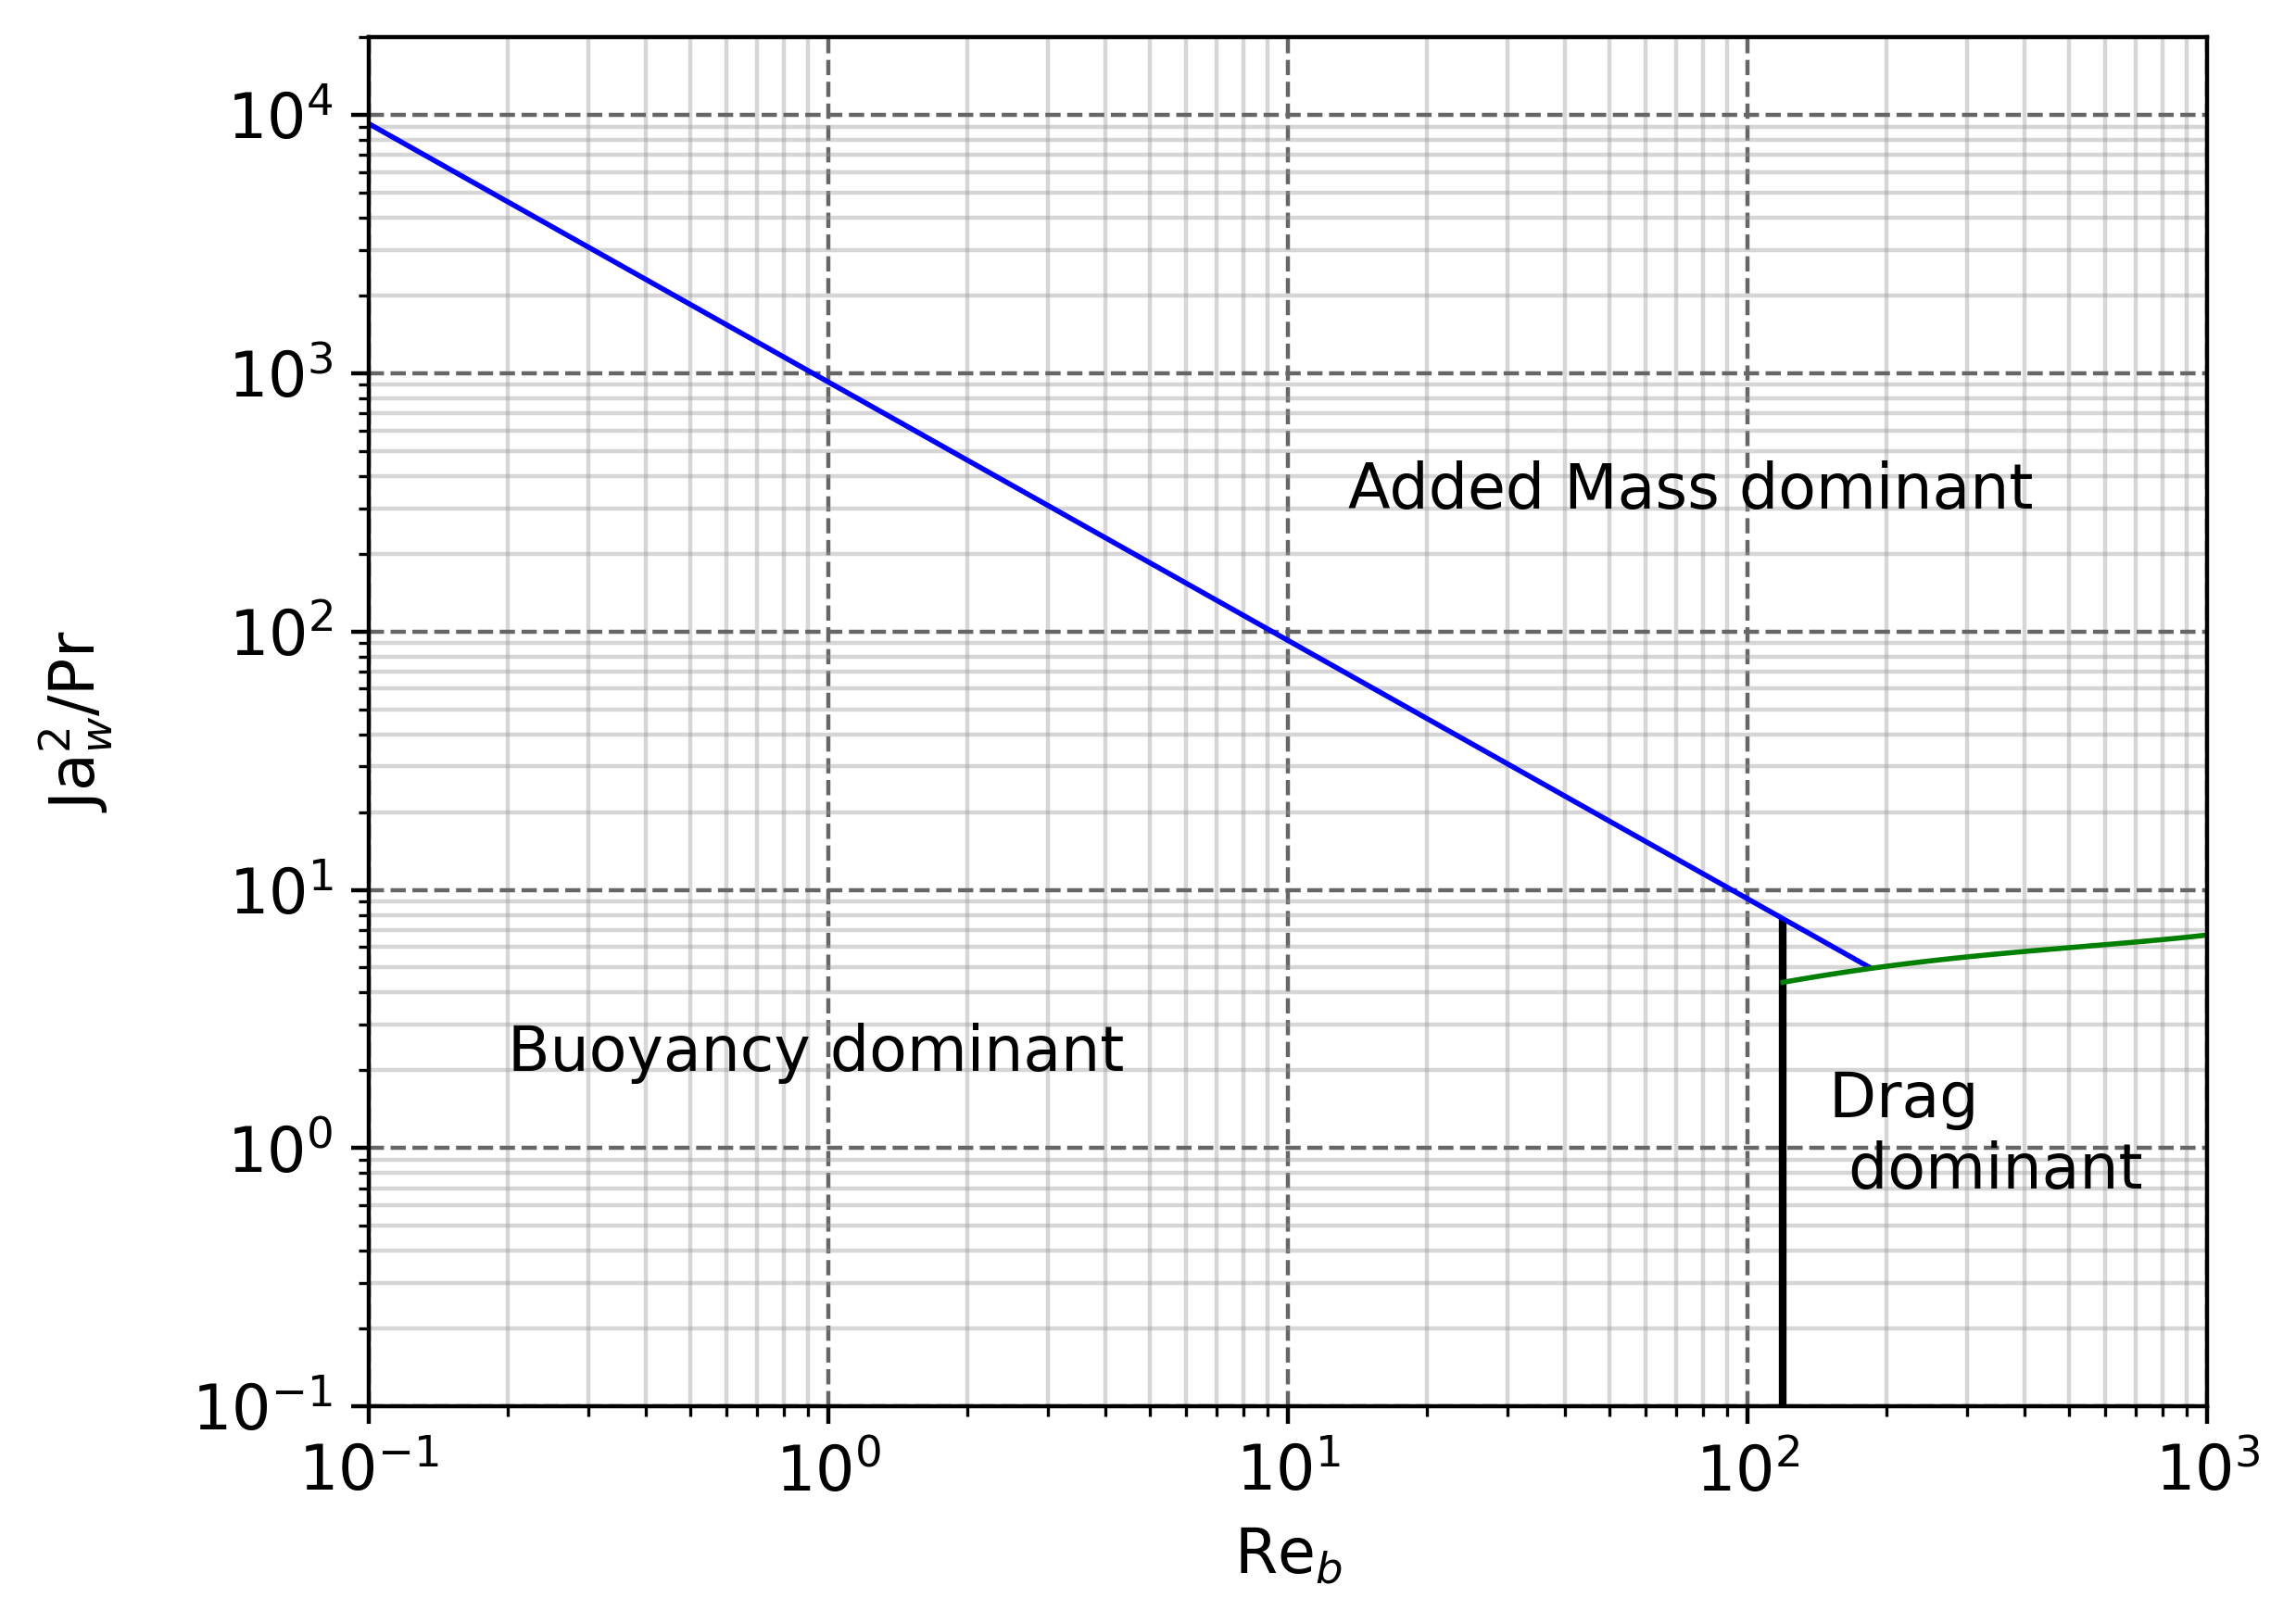
\includegraphics[width=0.49\linewidth]{img/forces/map_1bar_bis.png}
\hfill
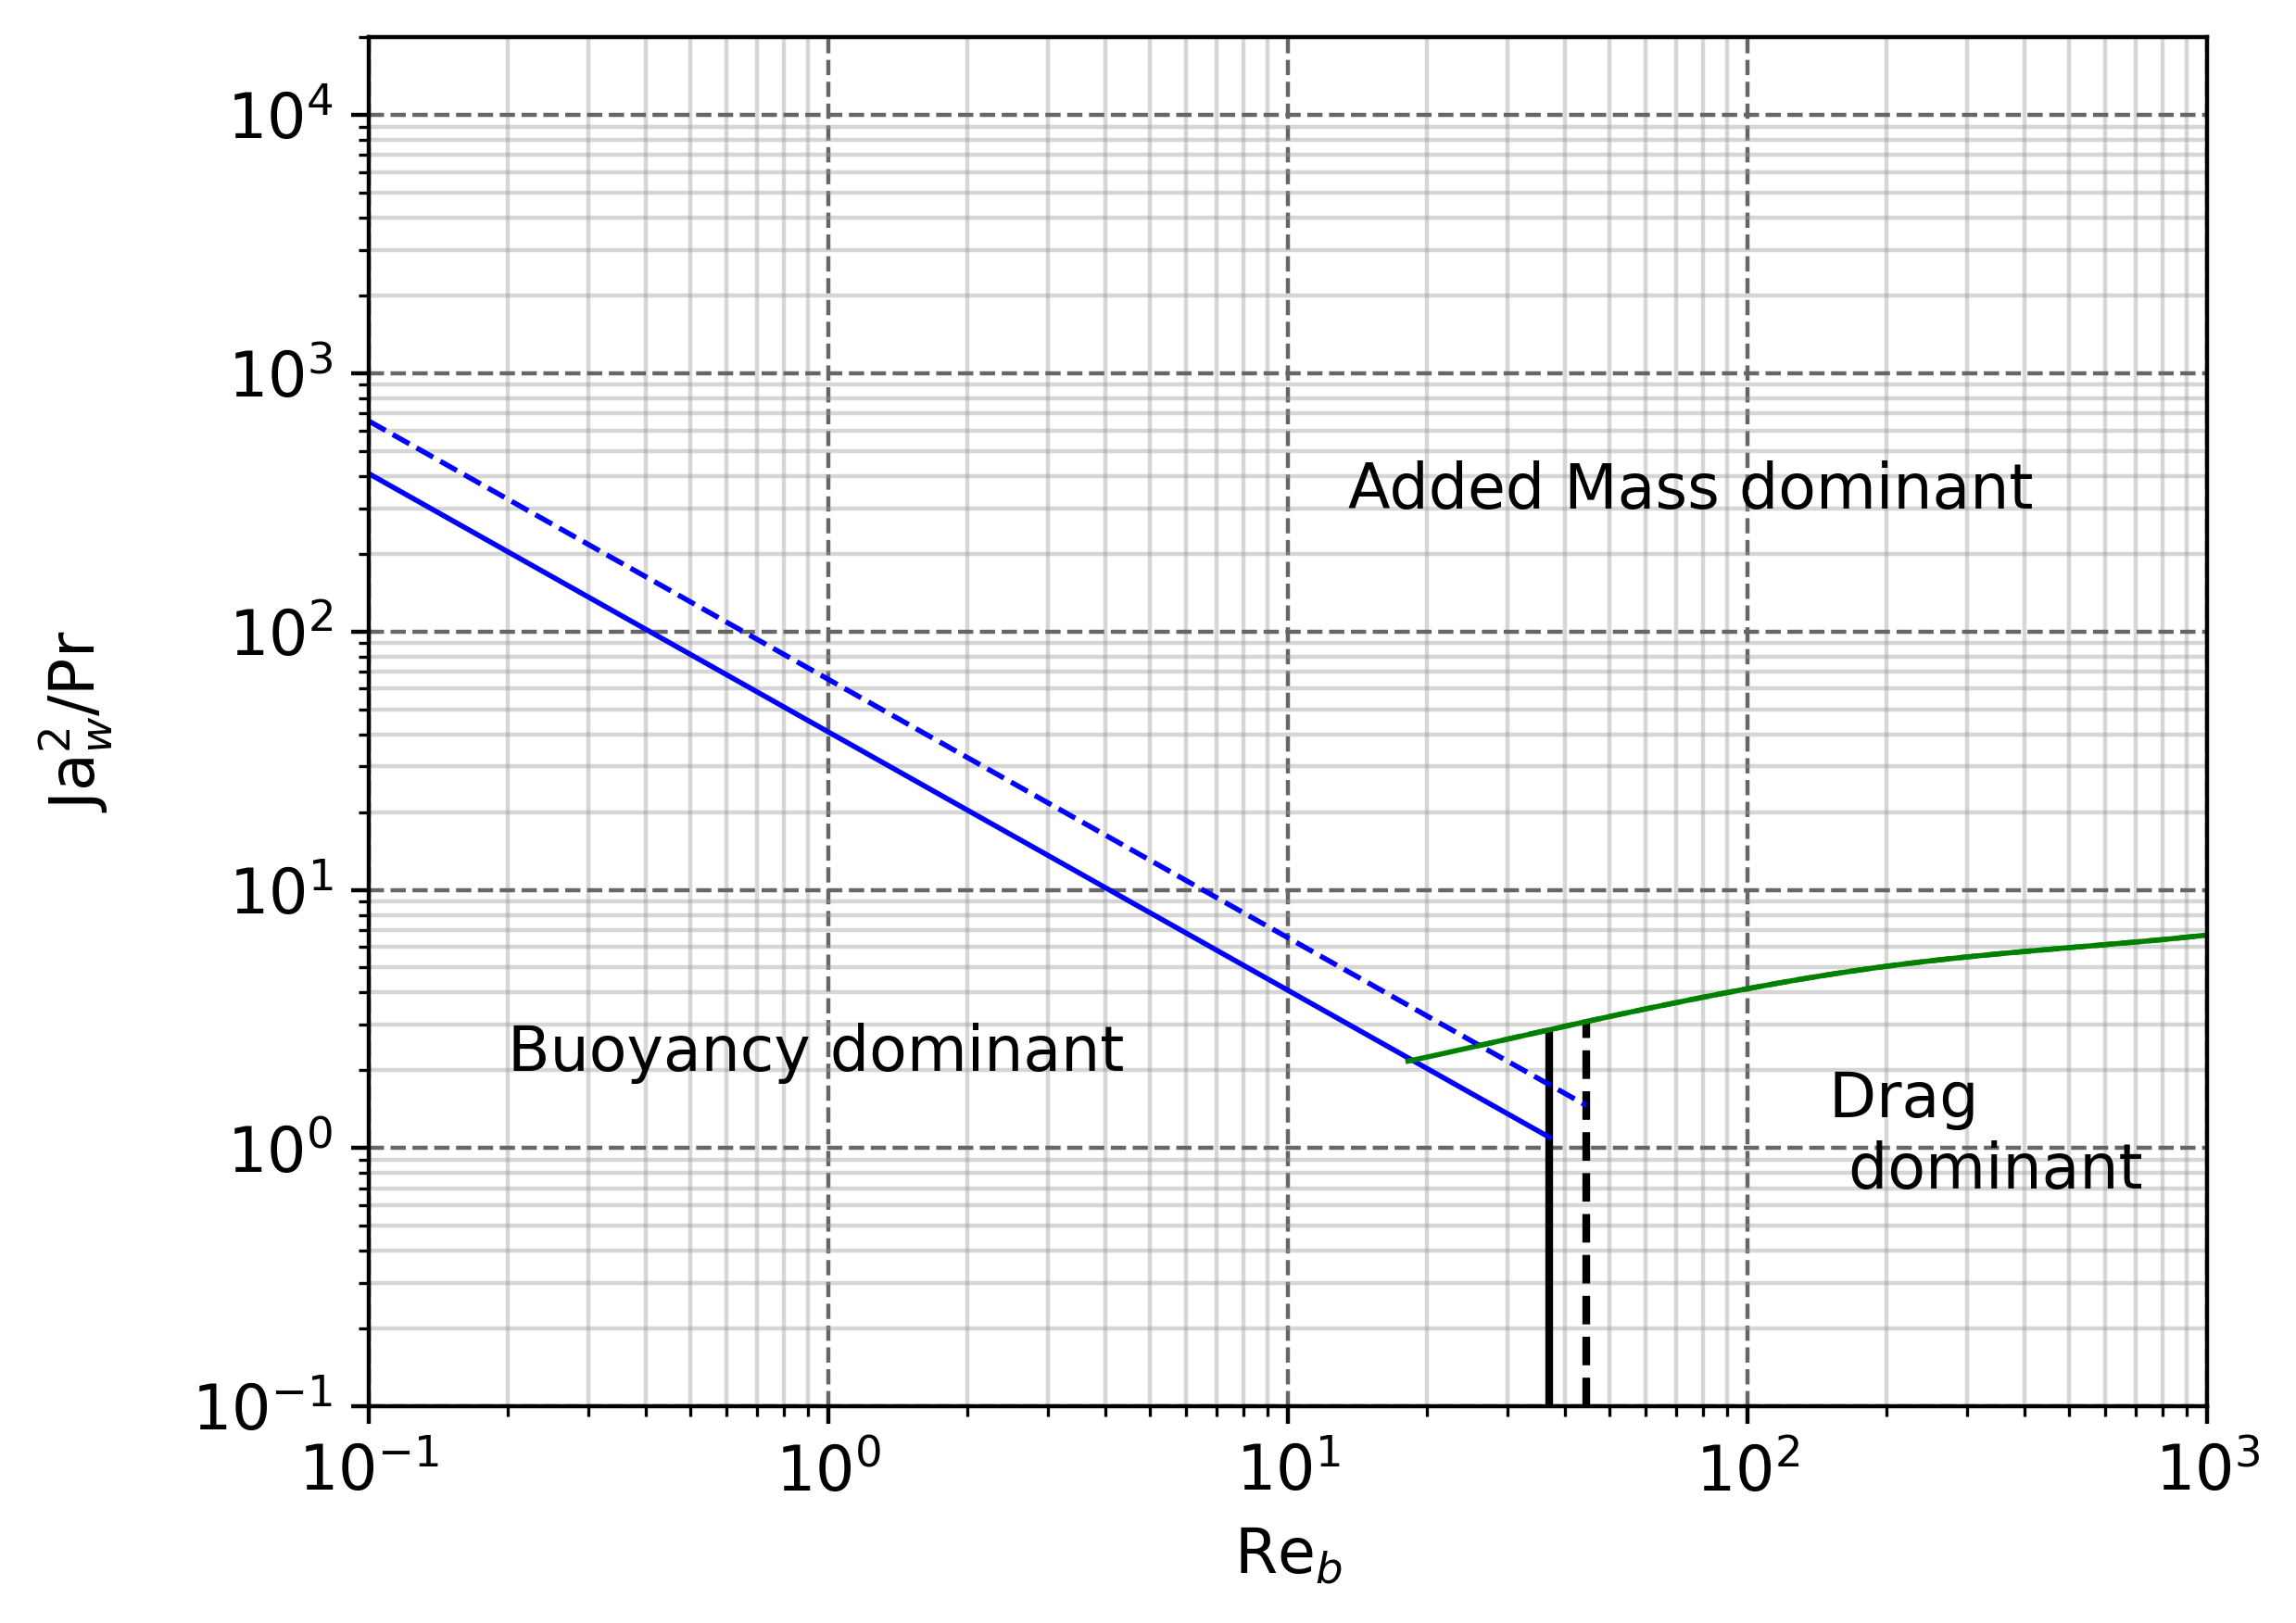
\includegraphics[width=0.49\linewidth]{img/forces/map_150bar_bis.png}
\caption{Force predominance map. Green, blue and black lines are respectively conditions (\ref{eq:AMvsD}),  (\ref{eq:AMvsB}) and (\ref{eq:DvsB}). Left represents $R=$0.25 mm for water at 1 Bar. Right represents $R=$0.05 mm, water at 150 Bar (plain lines) and R12 at 25 Bar (dashed lines).}
\label{fig:dom_slide}
\vspace{16pt}
\end{figure}

It appears that the increase in pressure along with the bubble diameter decrease leads to a larger range of flow parameters for which added mass effects and drag will be dominant. In addition, we also plotted the conditions for R12 at the similarity pressure of $26$ Bar where its properties such as $\We$ and $\rho_{L}/\rho_{V}$  are close to water in PWR conditions\cite{Garnier2001}. The proximity between the boundaries on Figure \ref{fig:dom_slide} interestingly indicates that \textit{bubbles in pressurized R12 tests are likely to behave very similarly to bubbles in PWR regarding their departure by sliding.}

It is also interesting to note that the frontier between added mass and drag defined by condition (\ref{eq:AMvsD}) remains unchanged for the different pressures, fluids and bubble radii.

\subsection{Application to Low Pressure Data}

In order to apply the predominance criteria, we gathered three data sets of experimental bubble departure diameter measurements in vertical flow boiling of water at atmospheric pressure. The associated experimental conditions are gathered on Table \ref{tab:exp_dd}. 

\vspace{16pt}
\begin{table}[!htb]
\centering
\caption{Thermal-hydraulics parameters range for the low pressure data.}
\vspace{14pt}
\begin{tabular}{|c||c|c|c|c||c|c|} \hline
Author &  $D_{h}$ (mm) & $G$ ($\debm$) & $\Delta T_{w}$ (K) & $D_{d}$ (mm)  & $\Re_{b}$ (-) & $\Ja_{w}^{2}/\Pr$ (-)\\
\hline
\hline
Sugrue \etal\cite{Sugrue2014} & 16.642 & 250 - 400 & 2 - 6 & 0.229 - 0.391 & 53.8 - 70.8 & 20.57 - 185.2 \\
\hline
Guan \etal\cite{Guan2014} & 9 & 87.3 - 319.2 & 4.5 - 8.5 & 0.62 - 1.85 & 75.9 - 406.02 & 104.2 - 371.6 \\
\hline
Maity\cite{Maity2000} & 20 & 0 - 239.6 & 5 - 5.9 & 0.788 - 1.713 & 0 - 241.04 & 128.6 - 179.06 \\
\hline
\end{tabular}
\label{tab:exp_dd}
\end{table}
\vspace{16pt}
To further justify the nearly-spherical shape hypothesis, we compute the range of Weber, Capillary and Eotvos numbers since they are representative of the deformability of the bubble under inertial, viscous and gravity effects (Table \ref{tab:exp_adim}).


\begin{table}[!htb]
\centering
\caption{Weber, Capillary and Eotvos numbers range for the low pressure data.}
\vspace{14pt}
\begin{tabular}{|c||c|c|c|}
\hline
Author & $\We$ (-) & $\Ca$ (-) & $\Eo$ (-)\\
\hline
\hline
Sugrue \etal\cite{Sugrue2014} & $6.36\times 10^{-3}$ - $12.6\times 10^{-3}$ & $2.22\times 10^{-4}$ - $3.64\times 10^{-4}$ & $2.09\times 10^{-3}$ - $6.09\times 10^{-3}$\\
\hline
Guan \etal\cite{Guan2014} & $3.79\times 10^{-3}$ - $82.8\times 10^{-3}$ & $0.998\times 10^{-4}$ - $4.93\times 10^{-4}$ & $1.53\times 10^{-2}$ - $13.6\times 10^{-2}$\\
\hline
Maity\cite{Maity2000} & $0$ - $3.5\times 10^{-2}$ & $0$ - $3.27 \times 10^{-4}$ & $2.48\times 10^{-2}$ - $11.7\times 10^{-2}$\\
\hline
\end{tabular}
\label{tab:exp_adim}
\end{table}
\vspace{16pt}


To compute the predominance boundaries as done in Figure \ref{fig:dom_slide}, we need to choose a bubble radius. Here we take the average departure radius of each data set to plot the associated boundaries. It appears that Guan and Maity data sets have very close average departure radius (approx. 0.6\ mm) and thus have the same predominance zones. The results are displayed on Figure \ref{fig:exp_dom}.
\begin{figure}[!htb]
\vspace{16pt}
\centering
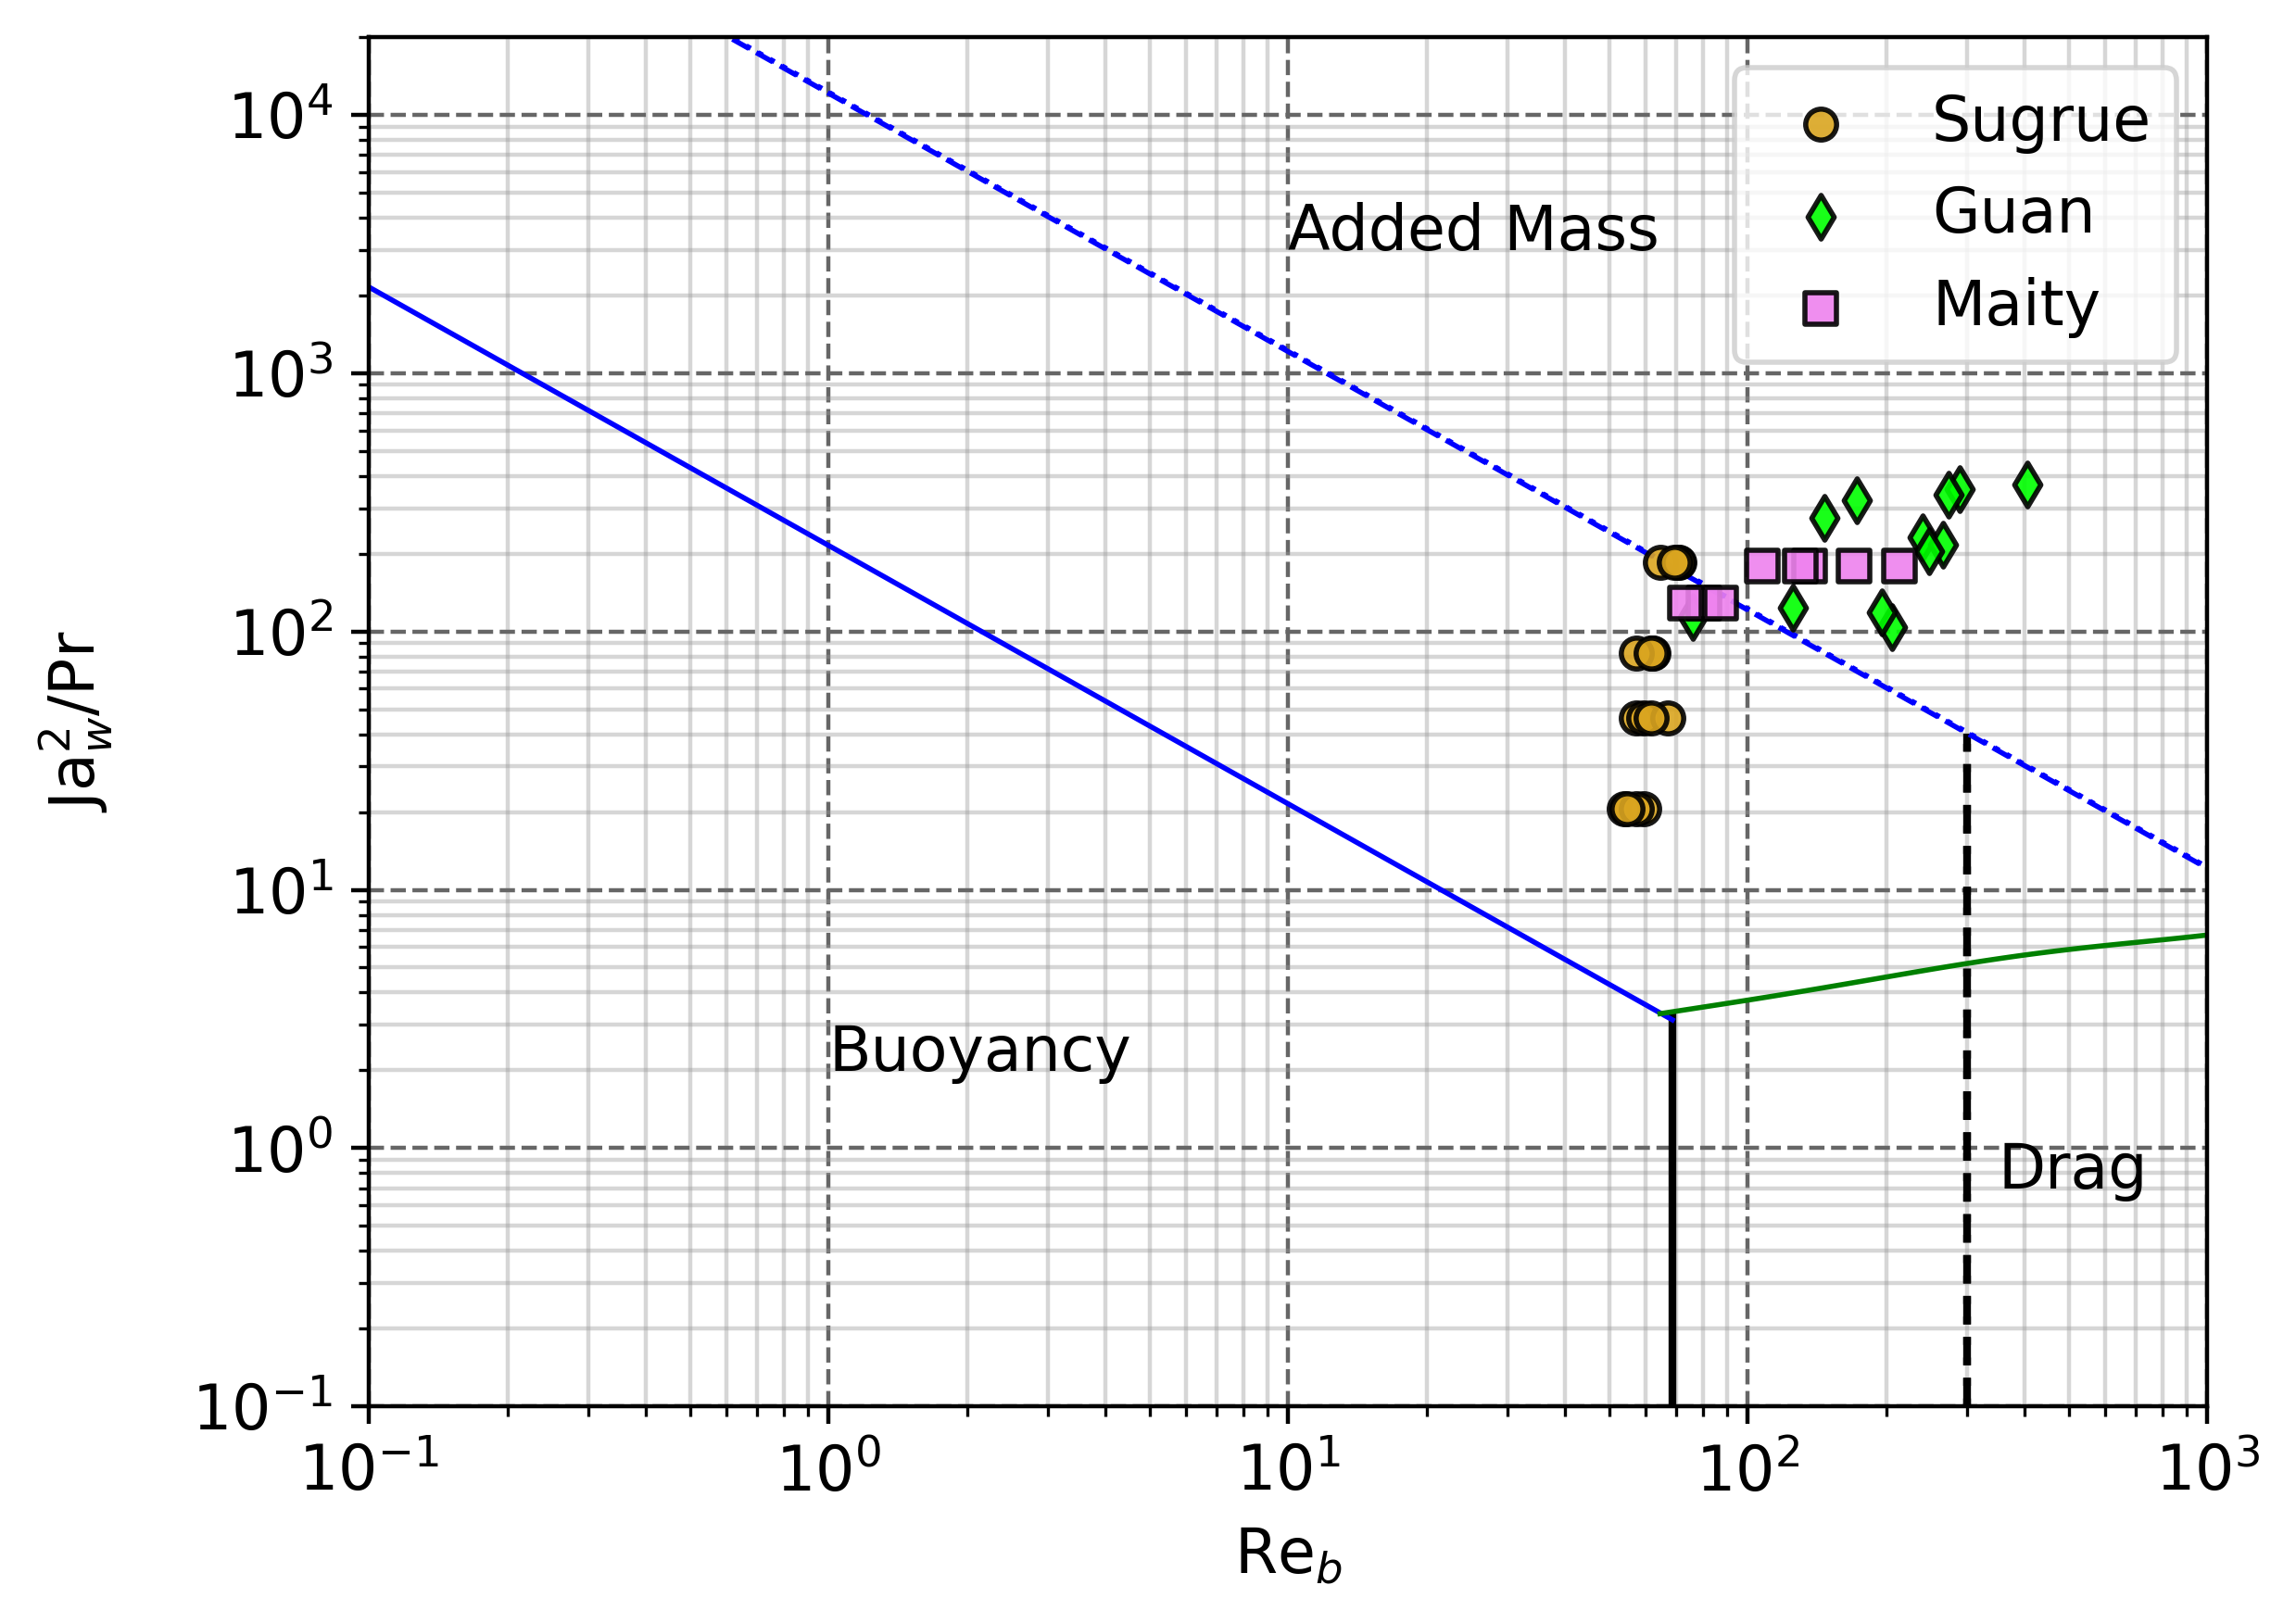
\includegraphics[width=0.6\linewidth]{img/forces/all_auth_map.png}
\caption{Experimental measurements in the dominance map. Plain lines correspond to Sugrue average departure radius (0.15 mm), dashed lines to Guan and Maity (0.59 mm).}
\label{fig:exp_dom}
\vspace{16pt}
\end{figure}

It immediately appears that when departure by sliding occurs, 32 measurements out of 37 seem to be dominated by added mass effects. The remaining 5 are buoyancy-dominant (Guan and Maity data) but placed really close to the added mass / buoyancy boundary on the map. This observation tends to indicates that at low pressure and mass fluxes, the departure by sliding could be triggered mostly by the added mass effects resulting of the coupling between the rapid initial bubble growth and the surrounding liquid velocity (Subsection \ref{subsec:AM}). 

This is mainly a consequence of the significant wall superheat reached in such boiling conditions along with high values of $\rho_{L}/\rho_{V}$, leading to high values of $\Ja_{w}^{2}/\Pr$. 


\subsection{Application to High Pressure Data}

Measurements of high-pressure bubble departure diameter are more difficult to find in the literature especially because of the great difficulty to provide clear visualization of individual bubbles when pressure increases, since bubbles are greatly reducing in size down to a few $\mu$m. 

Nevertheless, recent works such as those conducted by Kossolapov\cite{Kossolapov2021} have managed to conduct such measurements at pressures up to 39.8 Bar. To evaluate the forces responsible for sliding at higher pressures, closer to PWR operating conditions, we conduct the same analysis as we did with the low-pressure data. Experimental operations and non-dimensional numbers are summed up in Table \ref{tab:koss_exp}.

\begin{table}[!htb]
\centering
\caption{Thermal-hydraulics parameters and dimensionless numbers range for Kossolapov data.}
\vspace{14pt}
\begin{tabular}{|c||c|c|c|c||c|} \hline
Author &  $D_{h}$ (mm) & $G$ ($\debm$) & $P$ (Bar) & $D_{d}$ (mm)  & $\Re_{b}$ (-) \\
\hline
\hline
Kossolapov\cite{Kossolapov2021} & 11.78 & 500 - 2000 & 10.5 ; 19.9 ; 39.8 & 0.01 - 0.13 & 5.95 - 131.77\\
\hline
\end{tabular}
\vspace{14pt}
\begin{tabular}{|c|c|c|}
\hline
$\We$ (-) & $\Ca$ (-) & $\Eo$ (-)\\
\hline
\hline
$0.5\times 10^{-3}$ - $84.8\times 10^{-3}$ & $1.47\times 10^{-4}$ - $14.8\times 10^{-4}$ & $0.82\times 10^{-5}$ - $85\times 10^{-5}$\\
\hline
\end{tabular}
\label{tab:koss_exp}
\end{table}
\vspace{16pt}

Wall superheat or heat flux values are not specified in Kossolapov data because the given diameters were used to depict a global trend with pressure and mass flux. However, wall superheat at \textbf{Onset of Nucleate Boiling} can be roughly estimated using Frost \& Dzakowic correlation\cite{Frost1967} which yields approximately $\Delta T_{w}\approx $
4 K for water at $40$ Bar under a 1 MW/m$^{2}$ heat flux. To cover a tentatively large enough range of $\Ja_{w}^{2}/\Pr$ values, we will place the measurements from Kossolapov on the predominance map assuming three possible wall superheats : 1 K, 5 K and 10 K. 

The resulting map is displayed on Figure \ref{fig:koss_map}. In order to make it easier to interpret, we colored the stable added mass / drag boundary (\ref{eq:AMvsD}) in black and used 3 colors to distinguish between the three operating pressures. The arbitrary superheat are made distinct with the markers shapes.

\begin{figure}[!htb]
\vspace{16pt}
\centering
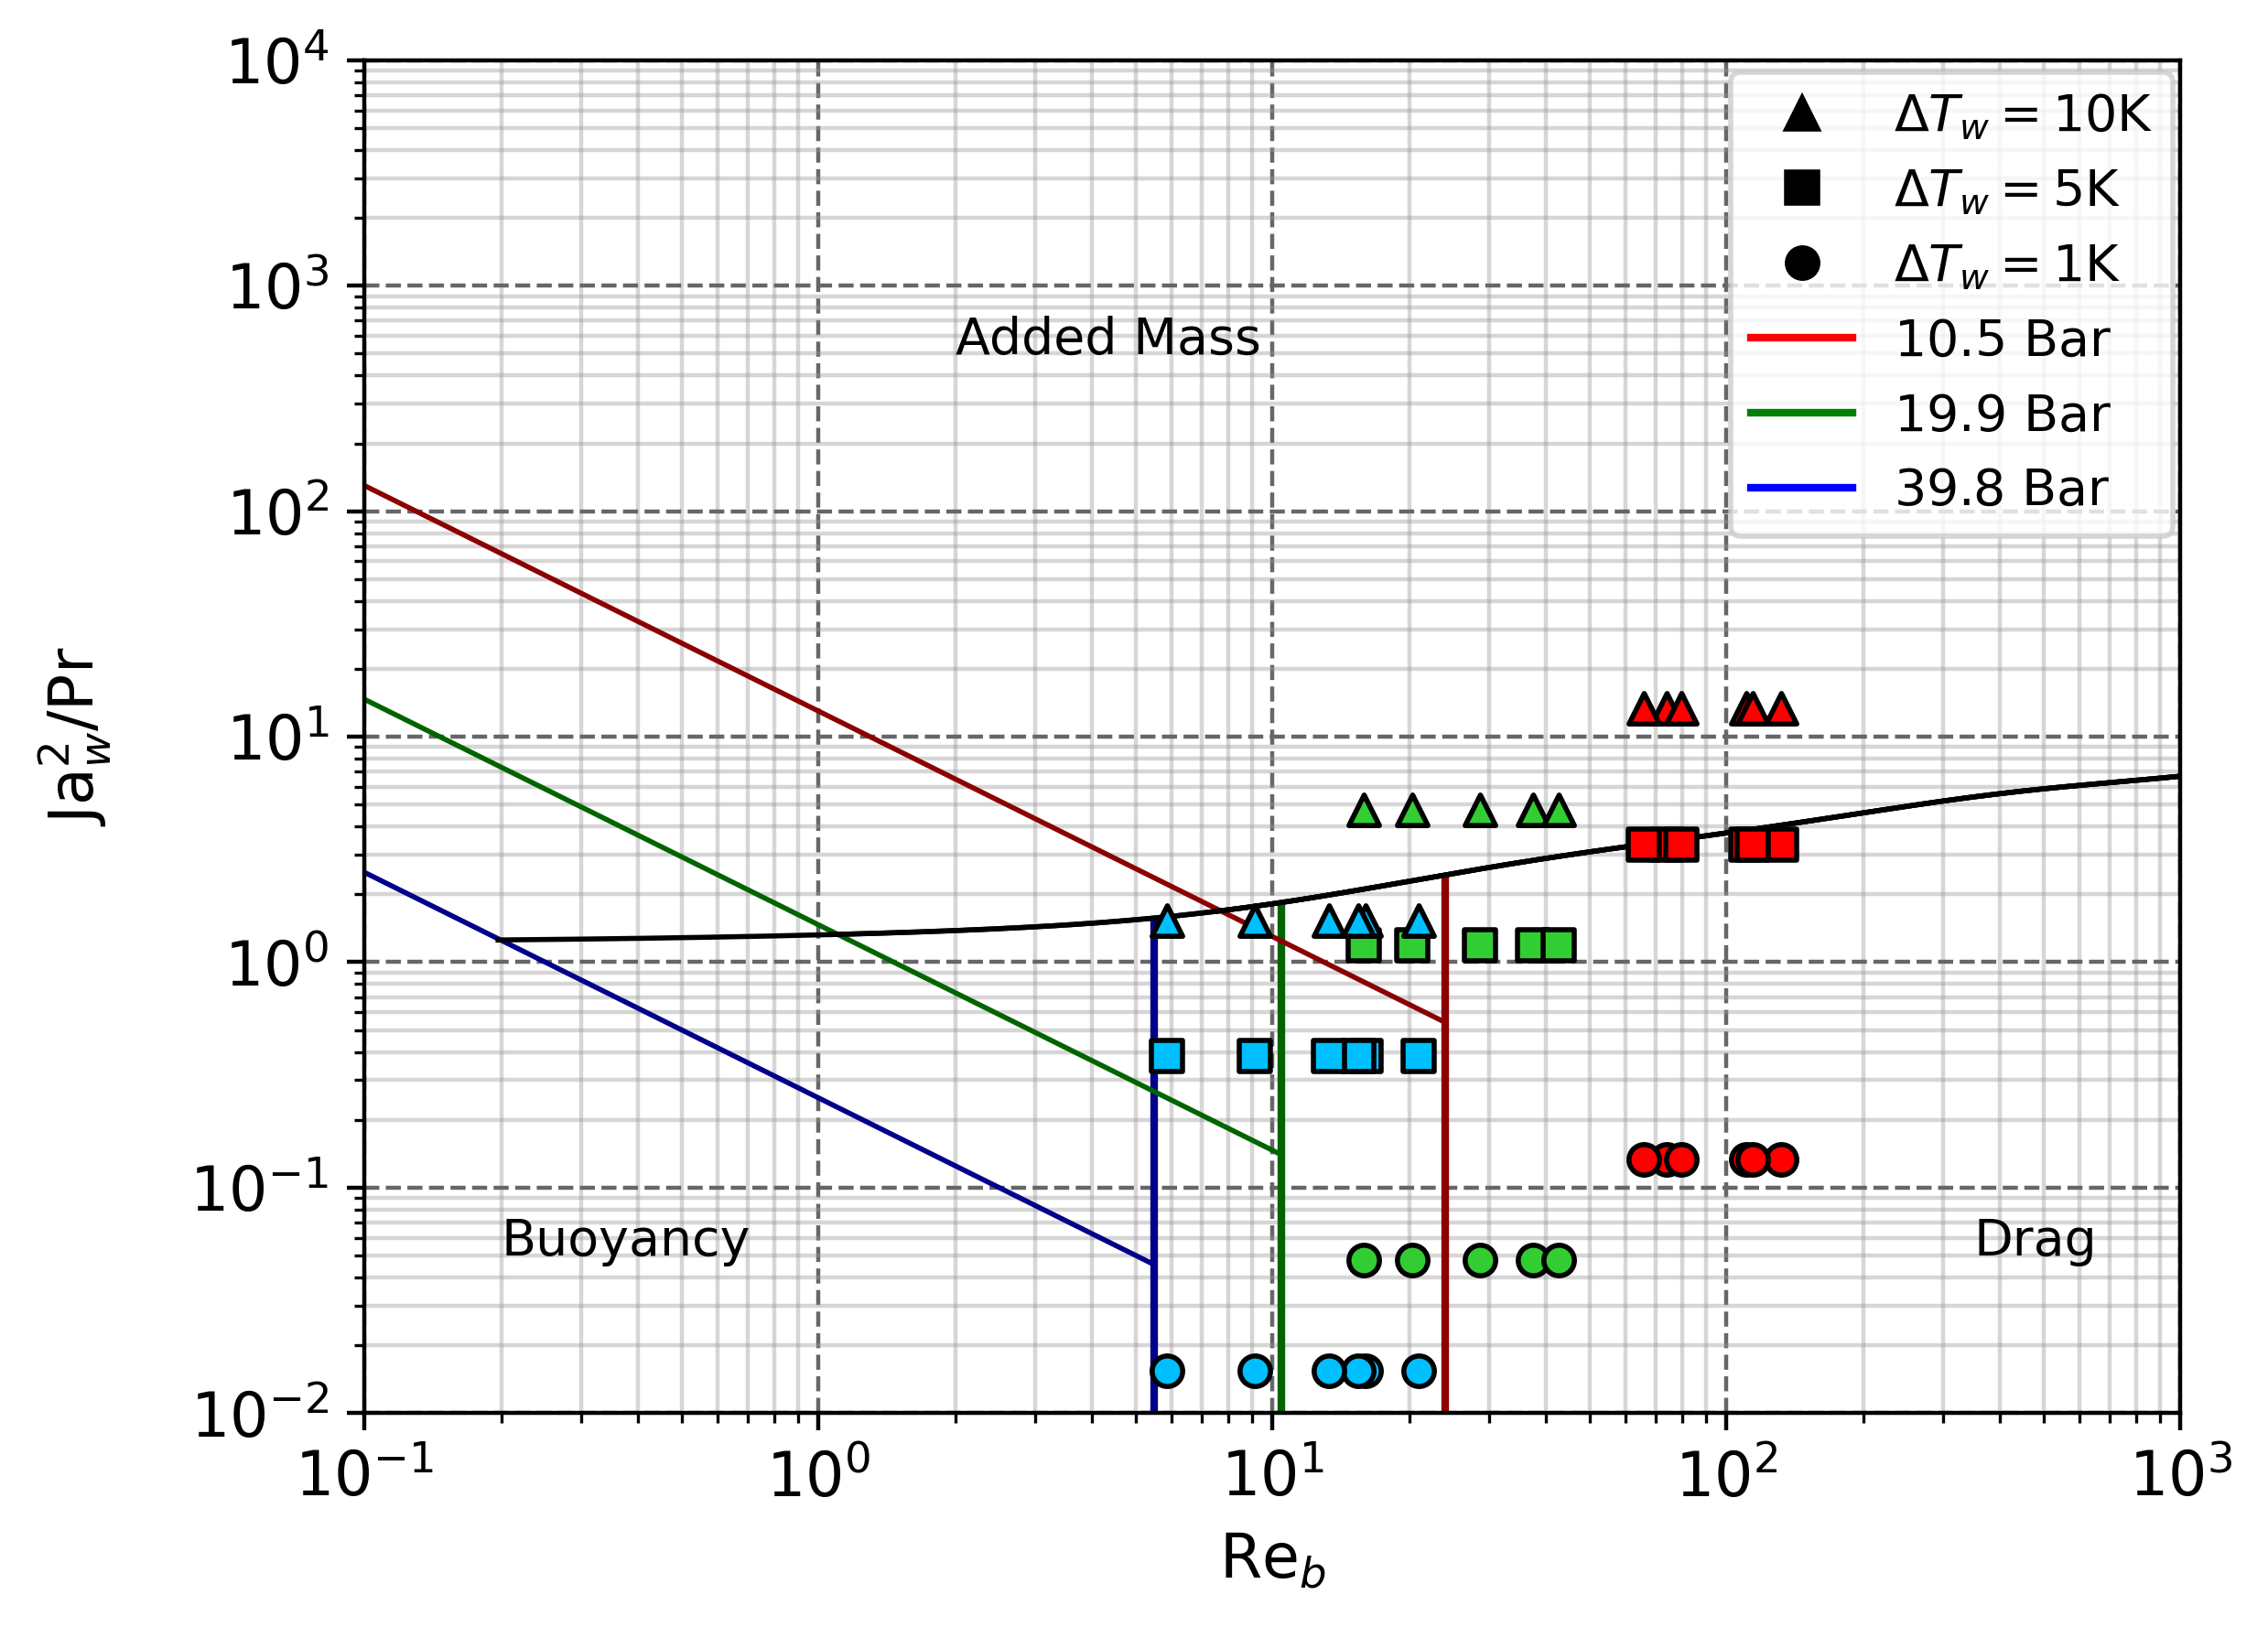
\includegraphics[width=0.6\linewidth]{img/forces/Koss_HP.png}
\caption{Experimental measurements from Kossolapov in the dominance map. Frontiers are plotted for the average departure radius at the given pressure. Blue : 39.8 Bar - Green : 19.9 Bar - Red : 10.5 Bar.}
\label{fig:koss_map}
\vspace{16pt}
\end{figure}

The main observation here relates to the values of $\Ja_{w}^{2}/\Pr$ which appear to be way smaller compared to the low pressure data, even for superheats as high as $10$K. This is mainly resulting from the strong decrease in the $\rho_{L}/\rho_{V}$ ratio with pressure, thus leading to predominance ranges where the force mostly responsible for departure by sliding is the drag. The higher mass fluxes also tend to increase this effect. Added mass only start to be significant under the 10 K superheat assumption.
%Moreover, we can note that the triangle-shaped zone corresponding to no clear dominance of one force against the other enlarges as the pressure increases.

Finally, this analysis of high pressure data tends to indicate that \emph{departure by sliding at high pressure is triggered in significantly different dynamic conditions in term of forces ratio (drag dominant) compared to low pressure (added mass dominant)}.

\section{Prediction of bubble departure diameter}
\label{sec:dd_pred}

The main goal of such a study would still remain to find a way to predict the departure diameter of bubbles in vertical flow boiling. Since only the capillary force is opposed to bubble departure, we can use non-dimensional force balance (\ref{eq:adim_bdf}) to search the maximum diameter above which :
\begin{equation}
 C_{AM,x}K^{2}\frac{\Ja_{w}^{2}}{\Pr}+\frac{\Re_{b}}{\Fr} + \frac{3}{8}C_{D}\Re_{b} > \frac{3}{2}\frac{f_{C,x}}{\Ca}
\label{eq:adim_dd}
\end{equation}

To compute $\Re_{b}$ and $C_{D}$, we use Reichardt's law\cite{Reichardt1951} for the wall liquid velocity and shear at a distance $y=R$. Diameters predictions results are displayed on Figure \ref{fig:pred_dd}. The supposed wall superheat for Kossolapov data is 1 K.

\begin{figure}[!htb]
\vspace{16pt}
\centering
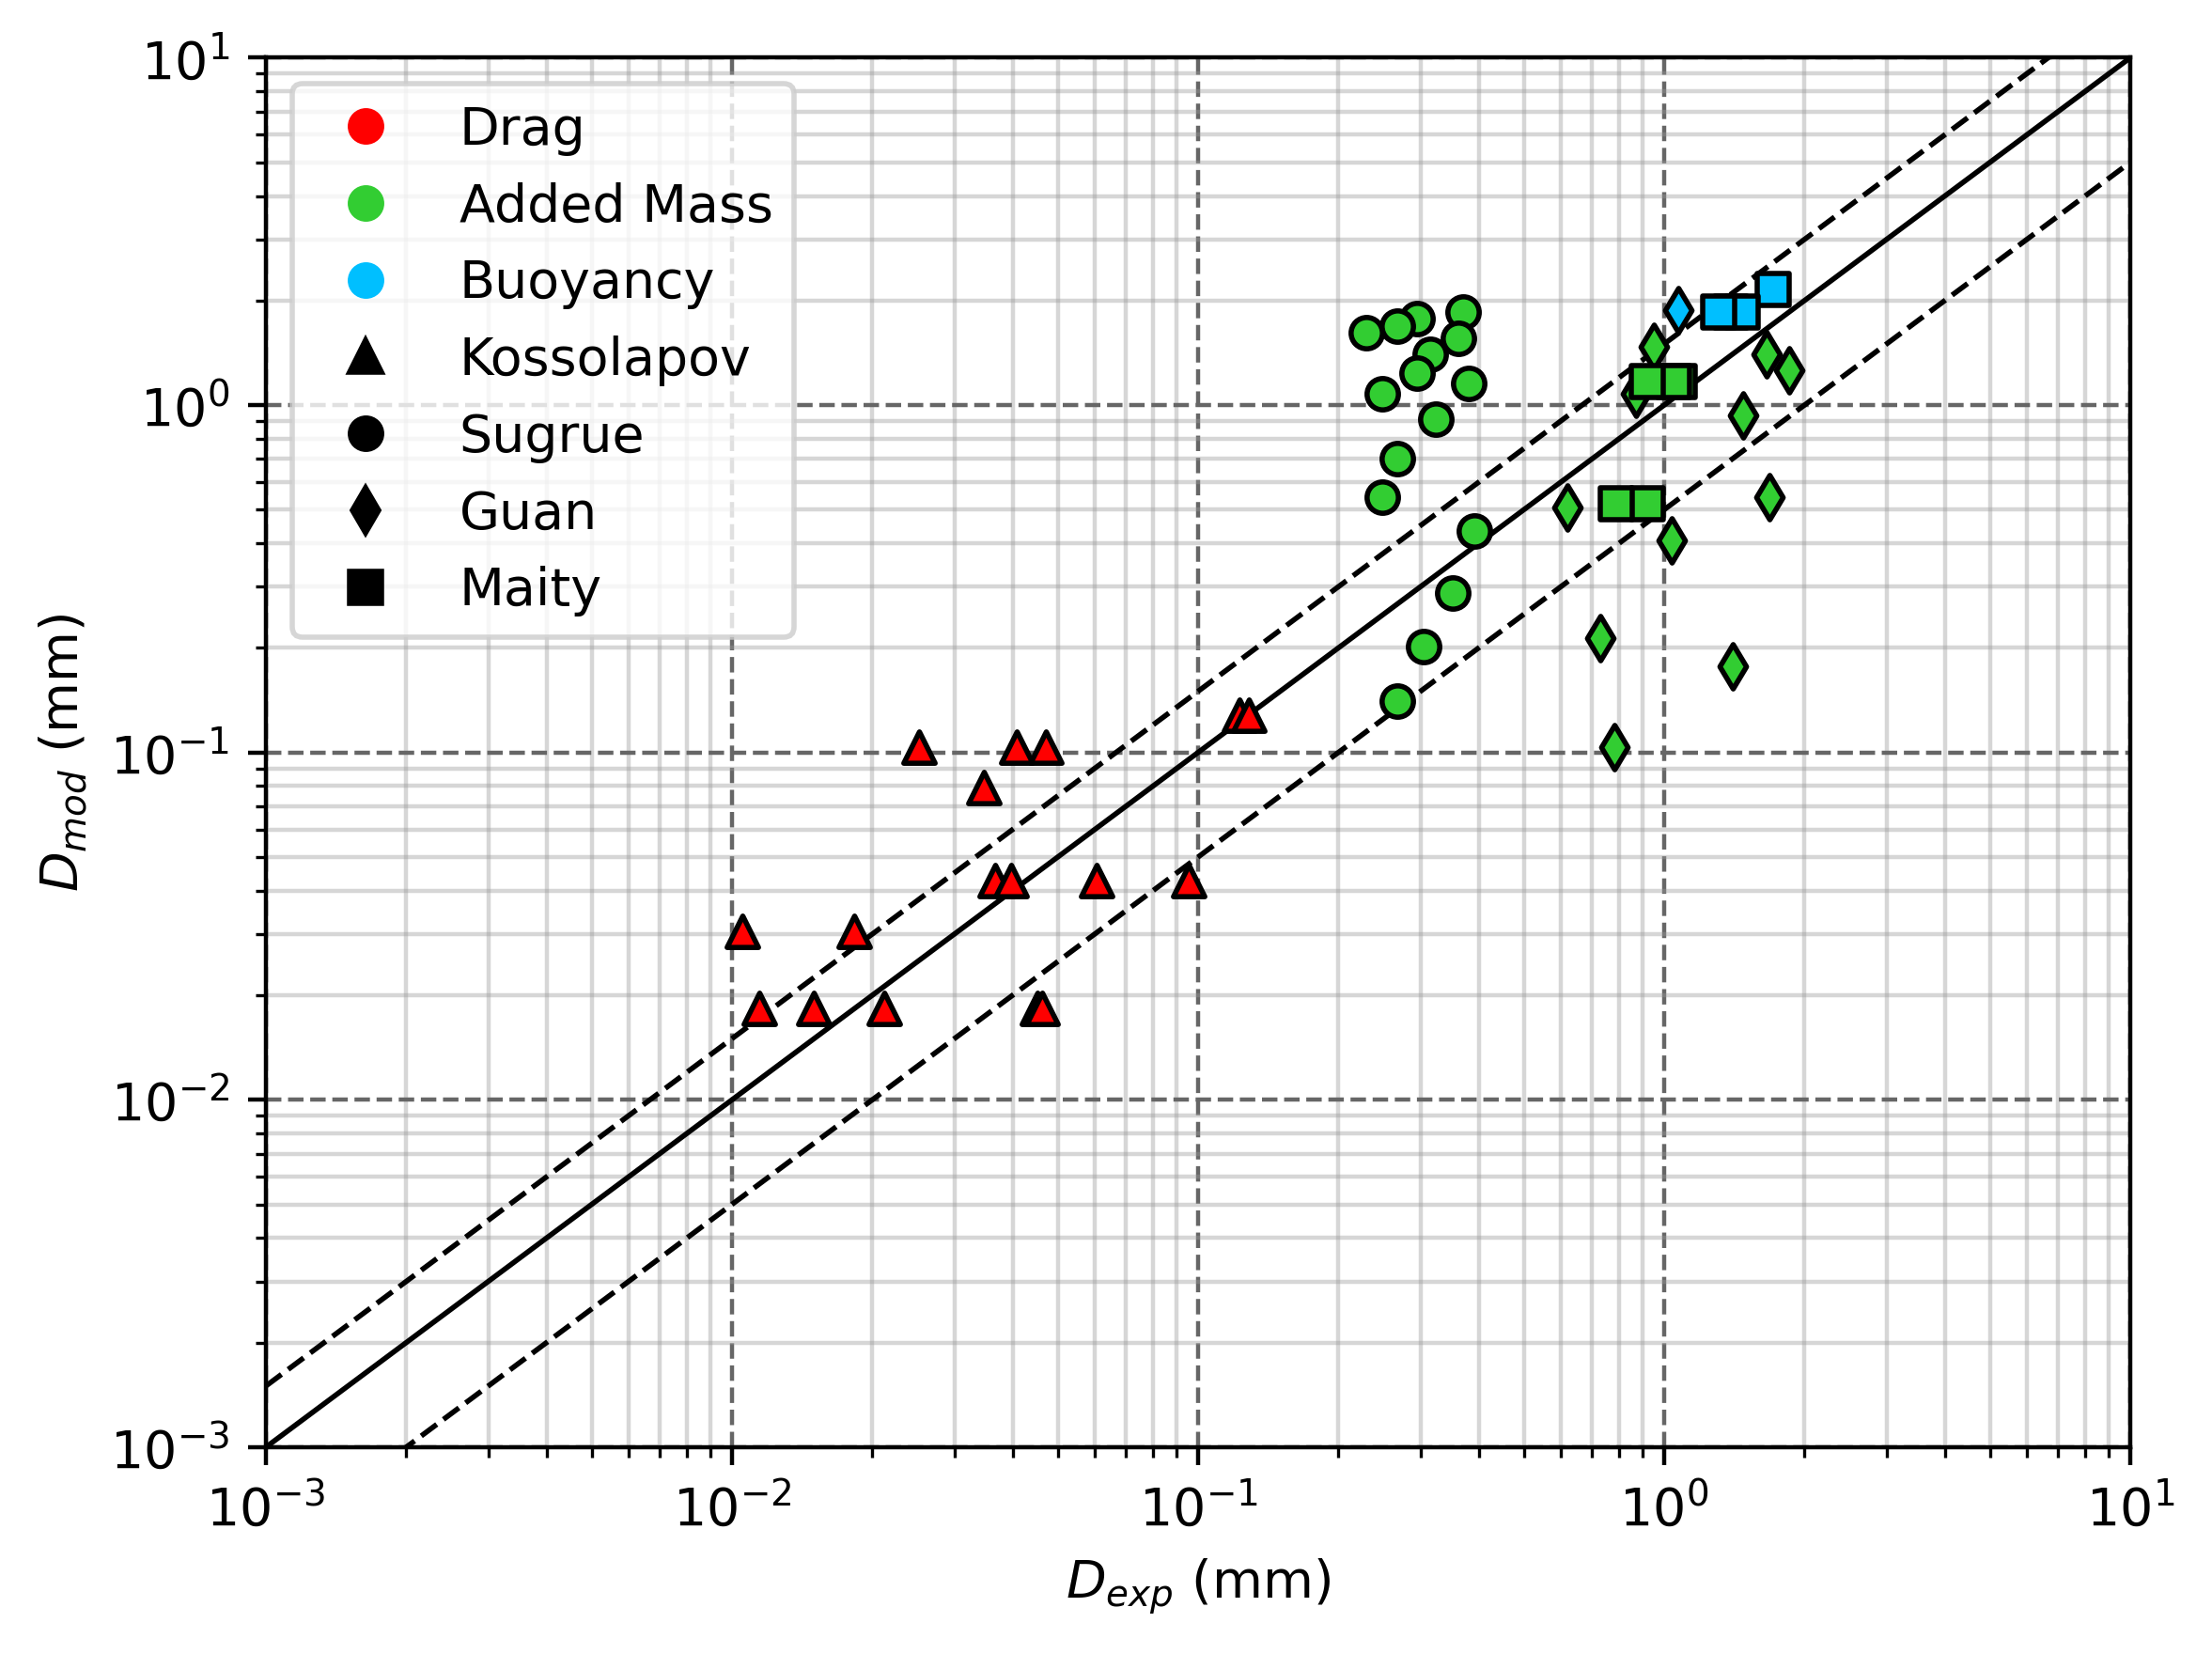
\includegraphics[width=0.49\linewidth]{img/forces/pred_dd_dom.png}
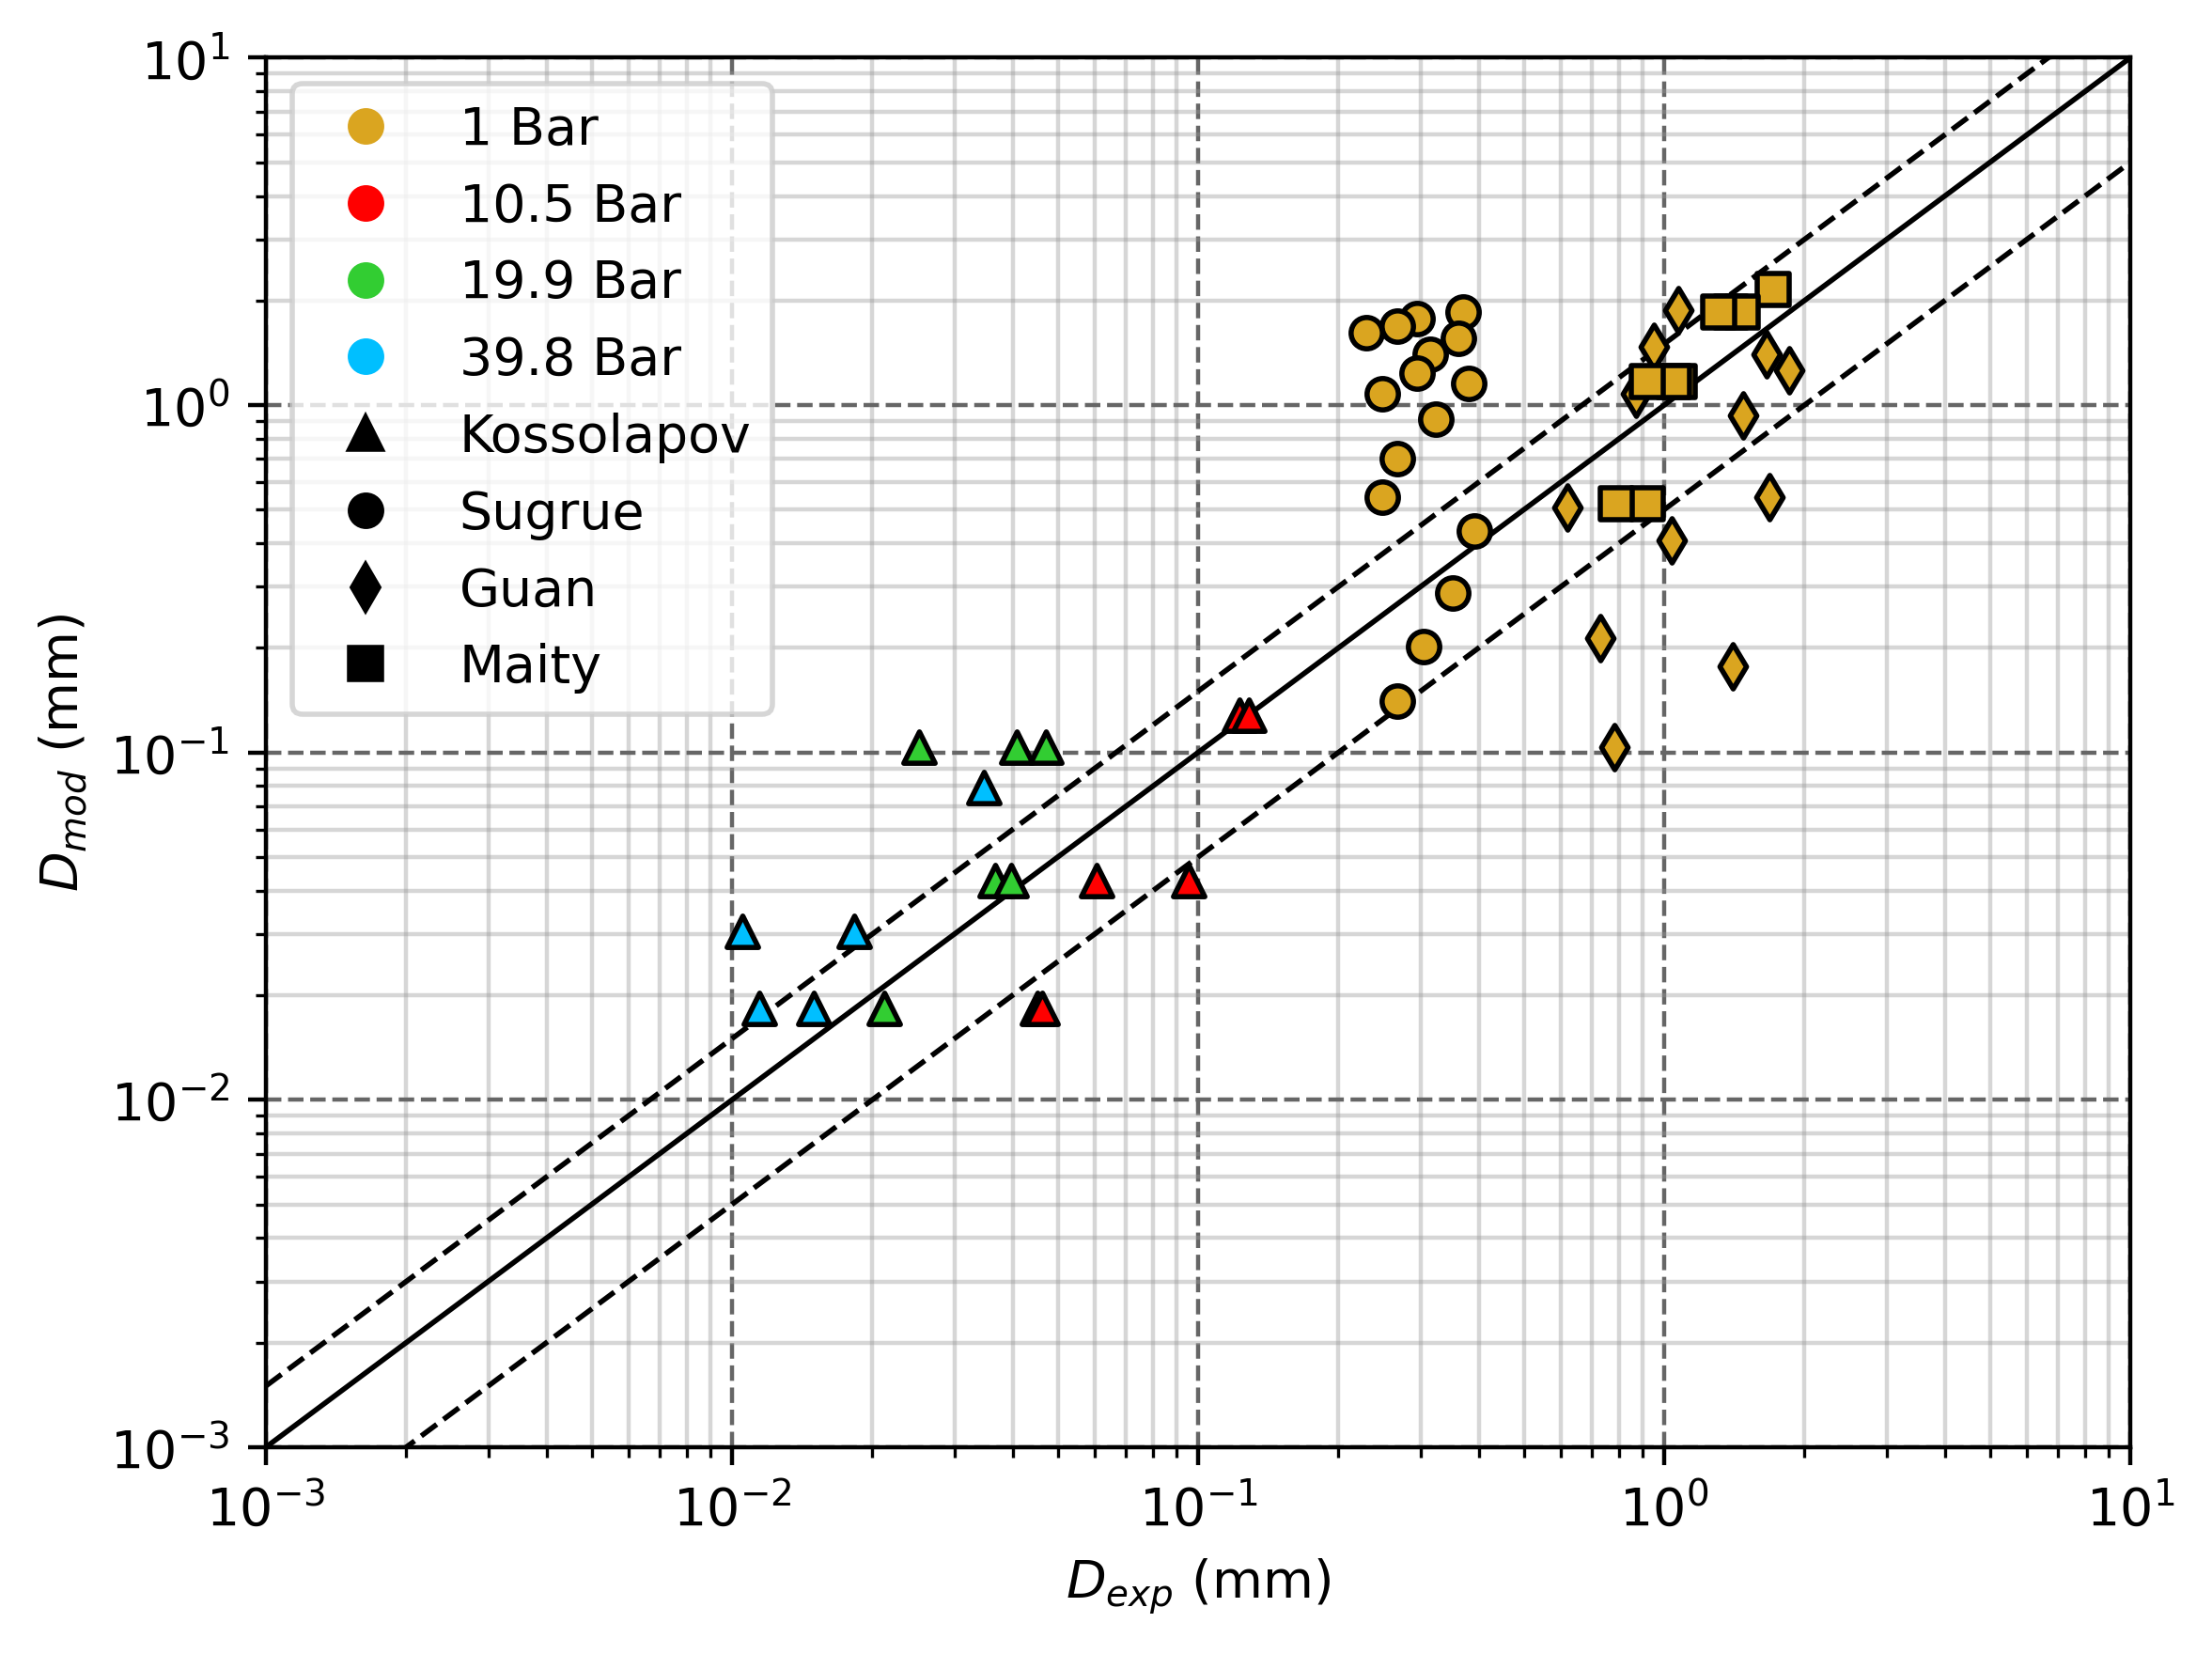
\includegraphics[width=0.49\linewidth]{img/forces/pred_dd_p.png}
\caption{Predicted diameter by Eq. \ref{eq:adim_dd} vs. experimental measurements. Colors refer to the dominant force at the departure by sliding (left) or to the operating pressure (right). $\pm 50\%$ error lines in dashed black.}
\label{fig:pred_dd}
\vspace{16pt}
\end{figure}

We can see that the predicted diameters seem to reasonably follow the global trend with pressure, which is an important feature in order to distinguish the different dynamic regimes depending on the flow conditions. 

The average contact and hysteresis angle used in the computations are $\theta=45\degree$, $\dtheta=36\degree$ for Sugrue's data (maximum hysteresis observed in her experiments) yielding an average error of 230.4\% ; $\theta=53\degree$, $\dtheta=27\degree$ for Guan's data (maximum hysteresis measured, accounting for uncertainties) yielding an average error of 182\% ; $\theta=60\degree$, $\dtheta=20\degree$ for Maity's data (average static angle, but increased hysteresis compared to the measurements) for an average error of 29.2\% ; $\theta=45\degree$, $\dtheta=1\degree$ for Kossolapov's data for an average error of 53.8\% (no measurements available).

Although the results seem to follow a correct trend with pressure, the average error can still be considered high on some data compared to other models\cite{Klausner1993}. However, such models often chose arbitrary values for parameters like the bubble foot diameter ($d_{w}=D/15$)\cite{Mazzocco2018} or the contact, hysteresis and inclination angles. Recent studies emphasized that such assumptions were substiantially wrong\cite{Bucci2021}. Moreover, those models consider an opposite contribution of the added mass regarding departure which seems to be incorrect as discussed earlier (Subsection \ref{subsec:AM}).

In this work, we insisted on keeping straight assumptions of a quasi-spherical bubble and to tried to apply the resulting laws for departure diameter prediction. \textbf{The only hypothetically free parameters were the average contact angle and hysteresis.} We tried to use author's data when available as inputs in our model. However, we did not have such measurements for Kossolapov's data and thus chose an average contact angle close to water FTO static contact angle (heater material used in his experiments) along with a very small hystersis, since very small bubbles in highly pressurized flow will be likely to keep non-deformed shapes because of surface tension effects getting stronger as the bubble diminishes in size. Moreover, we had to set a wall superheat which we chose to be $1$K (strongly drag-dominant regime).

Concerning the low pressure data, we observed that better results were obtained on Maity's measurements when using a bigger hysteresis angle. This may originate from the bubble foot diameter modeling, which was observed to be lower than the associated truncated sphere foot diameter in his experiments. In addition, the three low pressure data sets (Table \ref{tab:exp_dd}) have very close flow conditions, but significantly different measured departure diameter, especially when comparing Sugrue to Guan and Maity. The observed differences in experimental measurements can thus originate from the heater material, which impact is only indirectly included through the contact angle and hysteresis. This can explain the over-estimation of departure diameter on Sugrue's data when good agreement is observed with Guan and Maity. The same goes for the under-estimated diameters on Guan's data when we have a good agreement with Sugrue's measurements, explaining the high average relative deviation on those data sets.